\chapter{Search for Standard Model $\PH \to \Pgt\Pgt$}
\label{chap:httSM}

As discussed in chapter \ref{chap:theory}, the Higgs boson is the final missing 
piece of the Standard Model of particle physics. In order to complete the
\ac{SM}, the Higgs boson should have all the predicted properties of the
\ac{SM} Higgs, including decaying to predicted final states at the predicted rate. This
chapter describes the search for the Higgs boson of the Standard Model 
decaying into two tau leptons.

This chapter outlines the ``legacy'' \ac{SM} $\HToTauTau$ result from run 1 of the \ac{LHC}, using the
full dataset collected in 2011 and 2012 by CMS. This corresponds to an
integrated luminosity of 4.9 fb$^{-1}$ at a centre of mass energy of $7~\TeV$ and
19.7 fb$^{-1}$ at $8~\TeV$. The results in this chapter are parts of a publication 
in the Journal of High Energy Physics \cite{HIG-13-004}. The material included 
here is particularly focussed towards the parts of the analysis which 
included the work of the author. 

The $\PH \to \Pgt\Pgt$ analysis is performed in different final states dependent
on the final decay products of the taus. As discussed in section
\ref{sec:taus}, taus can decay into electrons $\Pe$,
muons $\Pmu$ and hadrons (denoted $\Pgth$), all with associated neutrinos.
This gives a total of six possible final states: $\ee$, $\mumu$, $\emu$,
$\etau$, $\mutau$ and $\tautau$. The most direct involvement of the author in this
analysis and the analyses described in the subsequent chapters was for the $\etau$ and
$\mutau$ channels, although considerable work was also done on the statistical
interpretation using the combination of results from all channels. 
As such the analysis details described in sections \ref{sec:eventSelection} to 
\ref{sec:systematics} are focussed on the
$\etau$ and $\mutau$ channels, whilst results including the combination of all
six $\HToTauTau$ channels, and additional channels from a dedicated $\PW\PH\to\Pgt\Pgt$ and
$\PZ\PH\to\Pgt\Pgt$ analysis, are shown in \ref{sec:results}. More detail on the other channels
can be found in \cite{HIG-13-004}. 

\section{Event Selection}
\label{sec:eventSelection}

This section describes how the objects discussed in chapter
\ref{chap:reco} are used to select the most signal-like events. 
%The selections used for the $\mutau$ and $\etau$ channels are discussed
%separately.

\subsection{Candidate Pair in the $\etau$ Channel}

Selected events in the $\etau$ channel require an electron and hadronic tau
candidate. The events are first selected by a trigger algorithm which requires
an electron and tau object. At the \ac{L1} trigger the requirement is simply a
single electron. At the \ac{HLT}, loose ID and isolation requirements are placed on the
electron, and additionally a $\Pgth$ object is required. For
the $\Pgth$ a simplified version of the \ac{PF} algorithm is used, and a loose
isolation is applied. These ID and isolation requirements are only approximate
compared to the more sophisticated algorithms which can be applied offline.  

In the offline selection the electron is required to have $\pt$ larger than ($20~\GeV$)
$24~\GeV$ in (2011) 2012 data. The higher $\pt$ cut in 2012 data is necessary
due to increased trigger thresholds necessary to maintain stable rates in the
higher instantaneous luminosity conditions. In all data taking periods the $\eta$ requirement
on the electron is $|\eta| < 2.1$. The electron is required to pass the electron
ID \ac{BDT} as described in section \ref{sec:electrons}, using a $\pt$ and
$\eta$ dependent cut which corresponds to the tight working point.  
The isolation definition described in section \ref{sec:leptonisolation} is
applied with a threshold of $I_{\text{rel}} < 0.1$. Finally, the electron must be compatible with
originating at the chosen \ac{PV}, and so the impact parameters in the
transverse and beam directions, $d_{xy}$ and $d_{z}$ respectively, must be 
less than $0.045~\cm$ and $0.2~\cm$. 

The selected hadronic tau has $\pt > 30~\GeV$ and $|\eta|<2.3$. 
The tau is identified using the \ac{HPS} algorithm as described in 
section \ref{sec:hps}. The tau must be compatible with
originating at the chosen \ac{PV}, and so the impact parameter in the beam
direction, $d_{z}$, must be smaller than $0.2~\cm$. 
As described in section \ref{sec:tauleptonrejection}, 
tau candidates are required to pass criteria to reduce the mis-identification of electrons and
muons. In the $\etau$ channel, a tight working point for electron rejection is
used, and a loose working point for muon rejection. Isolation as described in
section \ref{sec:tauisolation} is applied using an optimised working point of
$1.5~\GeV$.  

The electron and hadronic tau are required to be of opposite charge. If more
than one such pair exists in the event, then the pair with the highest sum $\pt$
is selected. The $\pt$ and $\eta$ distributions of the selected pair in the
$\etau$ channel are shown in figure \ref{fig:etauelectrons} for the electron and
\ref{fig:etautaus} for the tau. 


\begin{figure}[htb]
\begin{center}
\subfloat[]{
    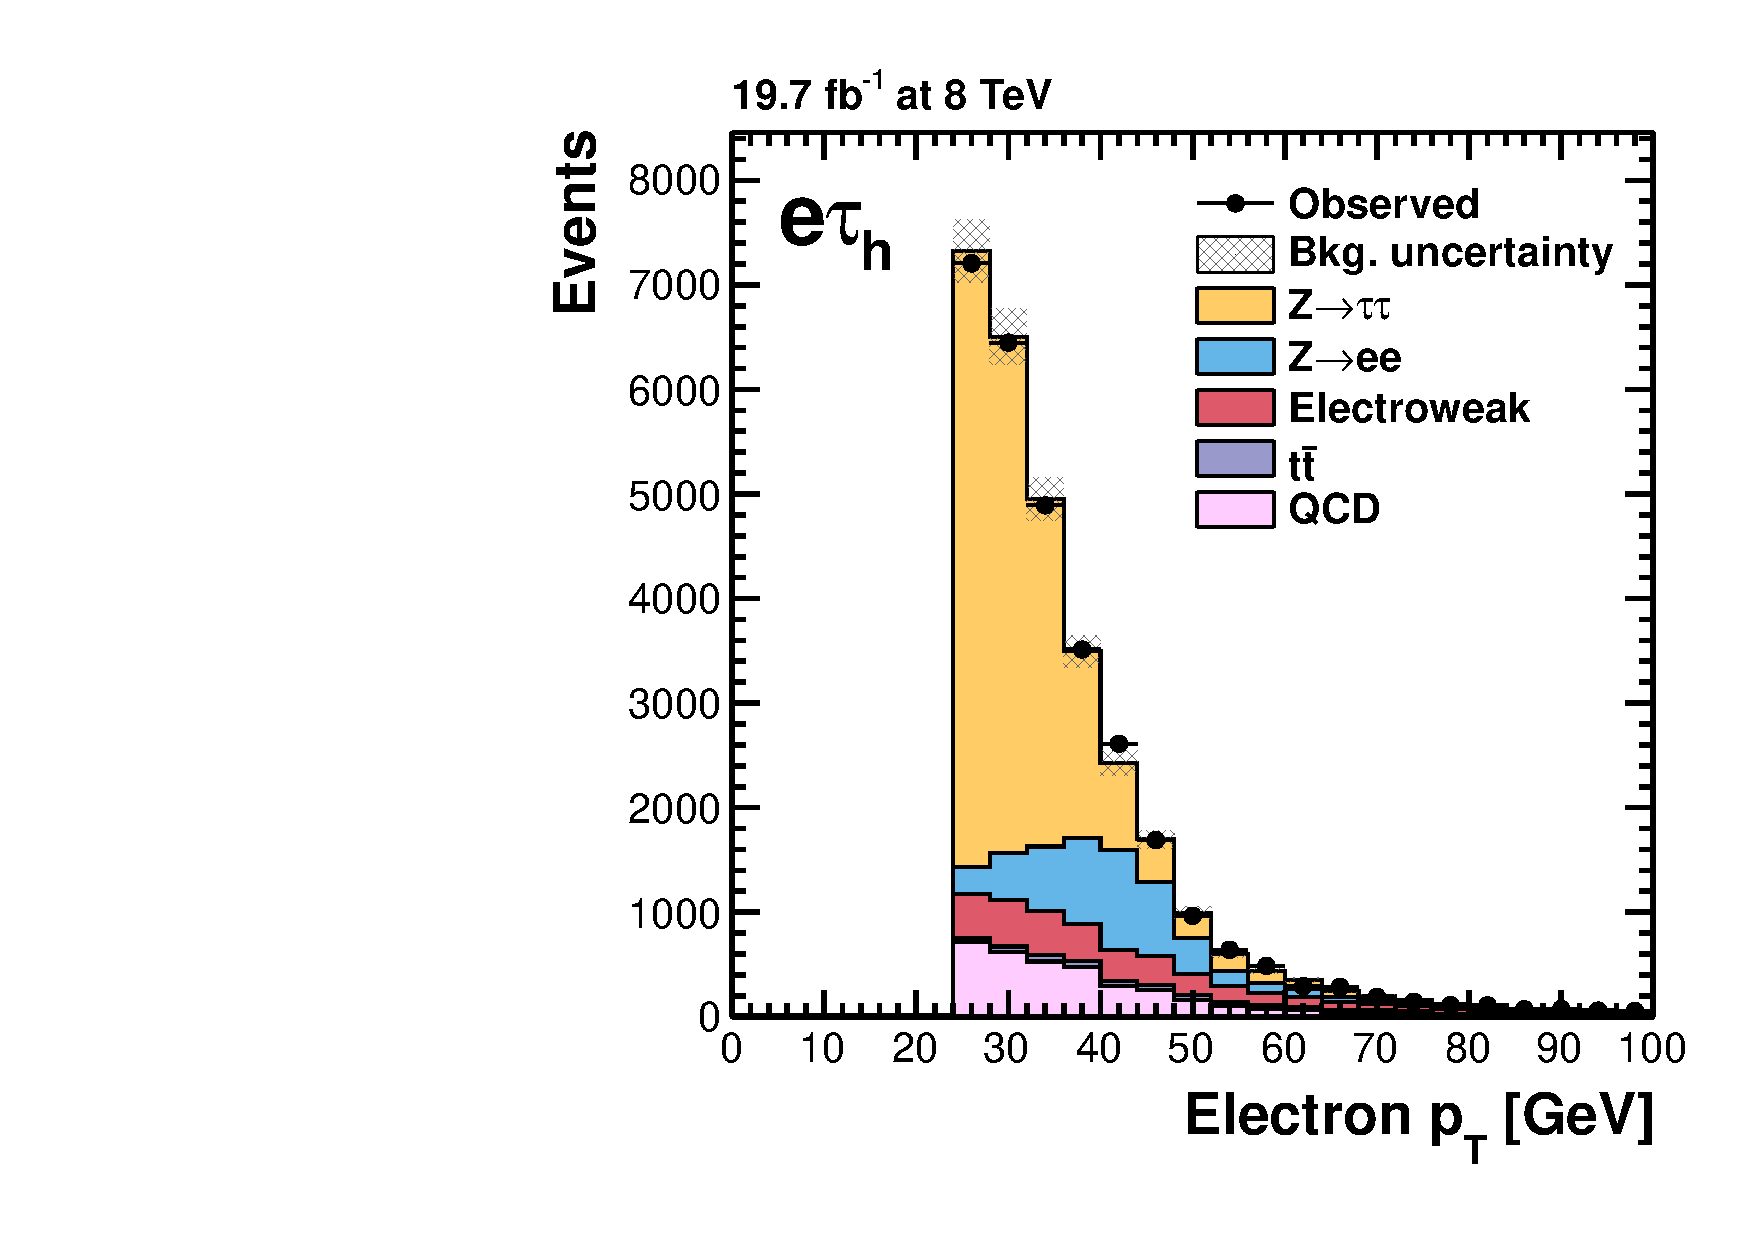
\includegraphics[width=0.5\textwidth]
      {plots/htt-sm/pt_1_inclusive_et_2012.pdf}}
\subfloat[]{
    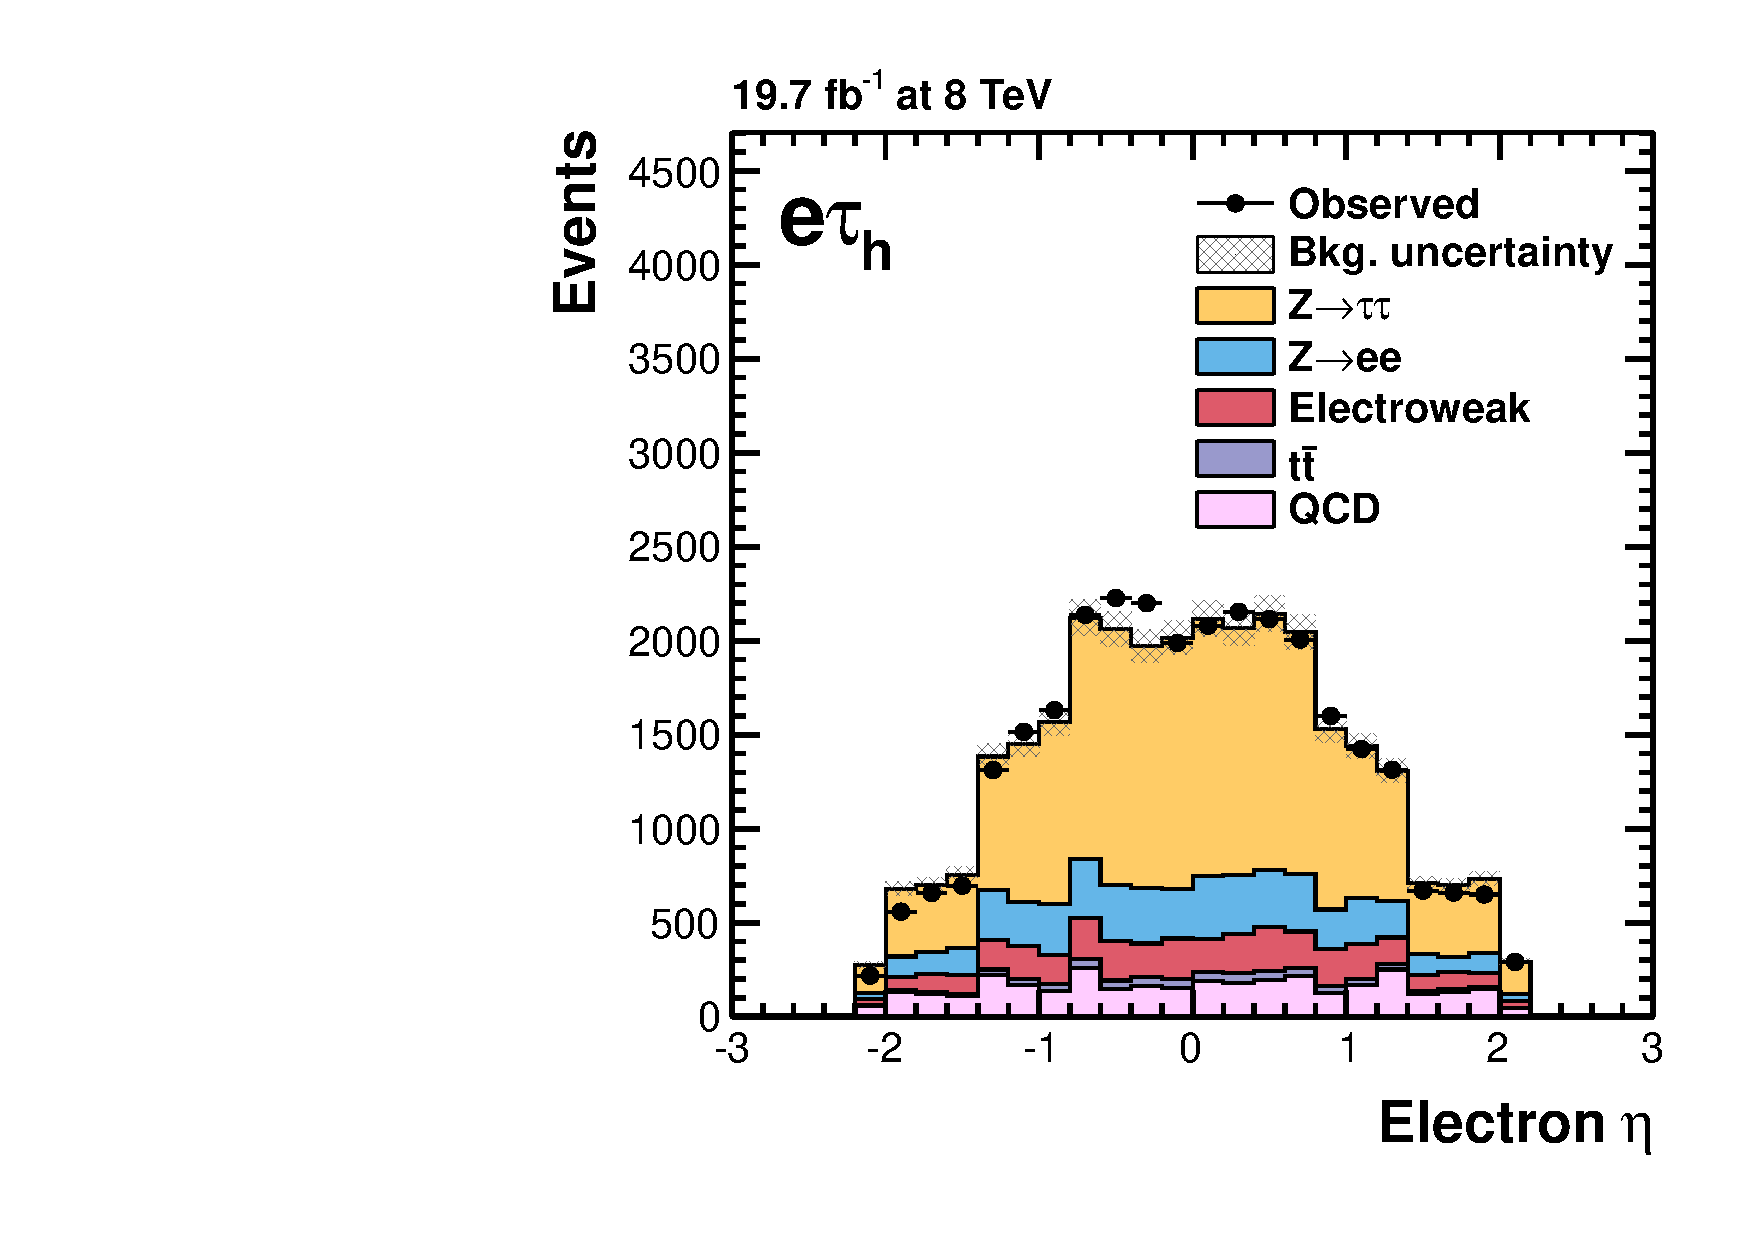
\includegraphics[width=0.5\textwidth] 
      {plots/htt-sm/eta_1_inclusive_et_2012.pdf}} 

\end{center}
\caption{
The $\pt$ and $\eta$ distribution for electron candidates in the $\etau$
channel.
}
\label{fig:etauelectrons}
\end{figure}


\begin{figure}[htb]
\begin{center}
\subfloat[]{
    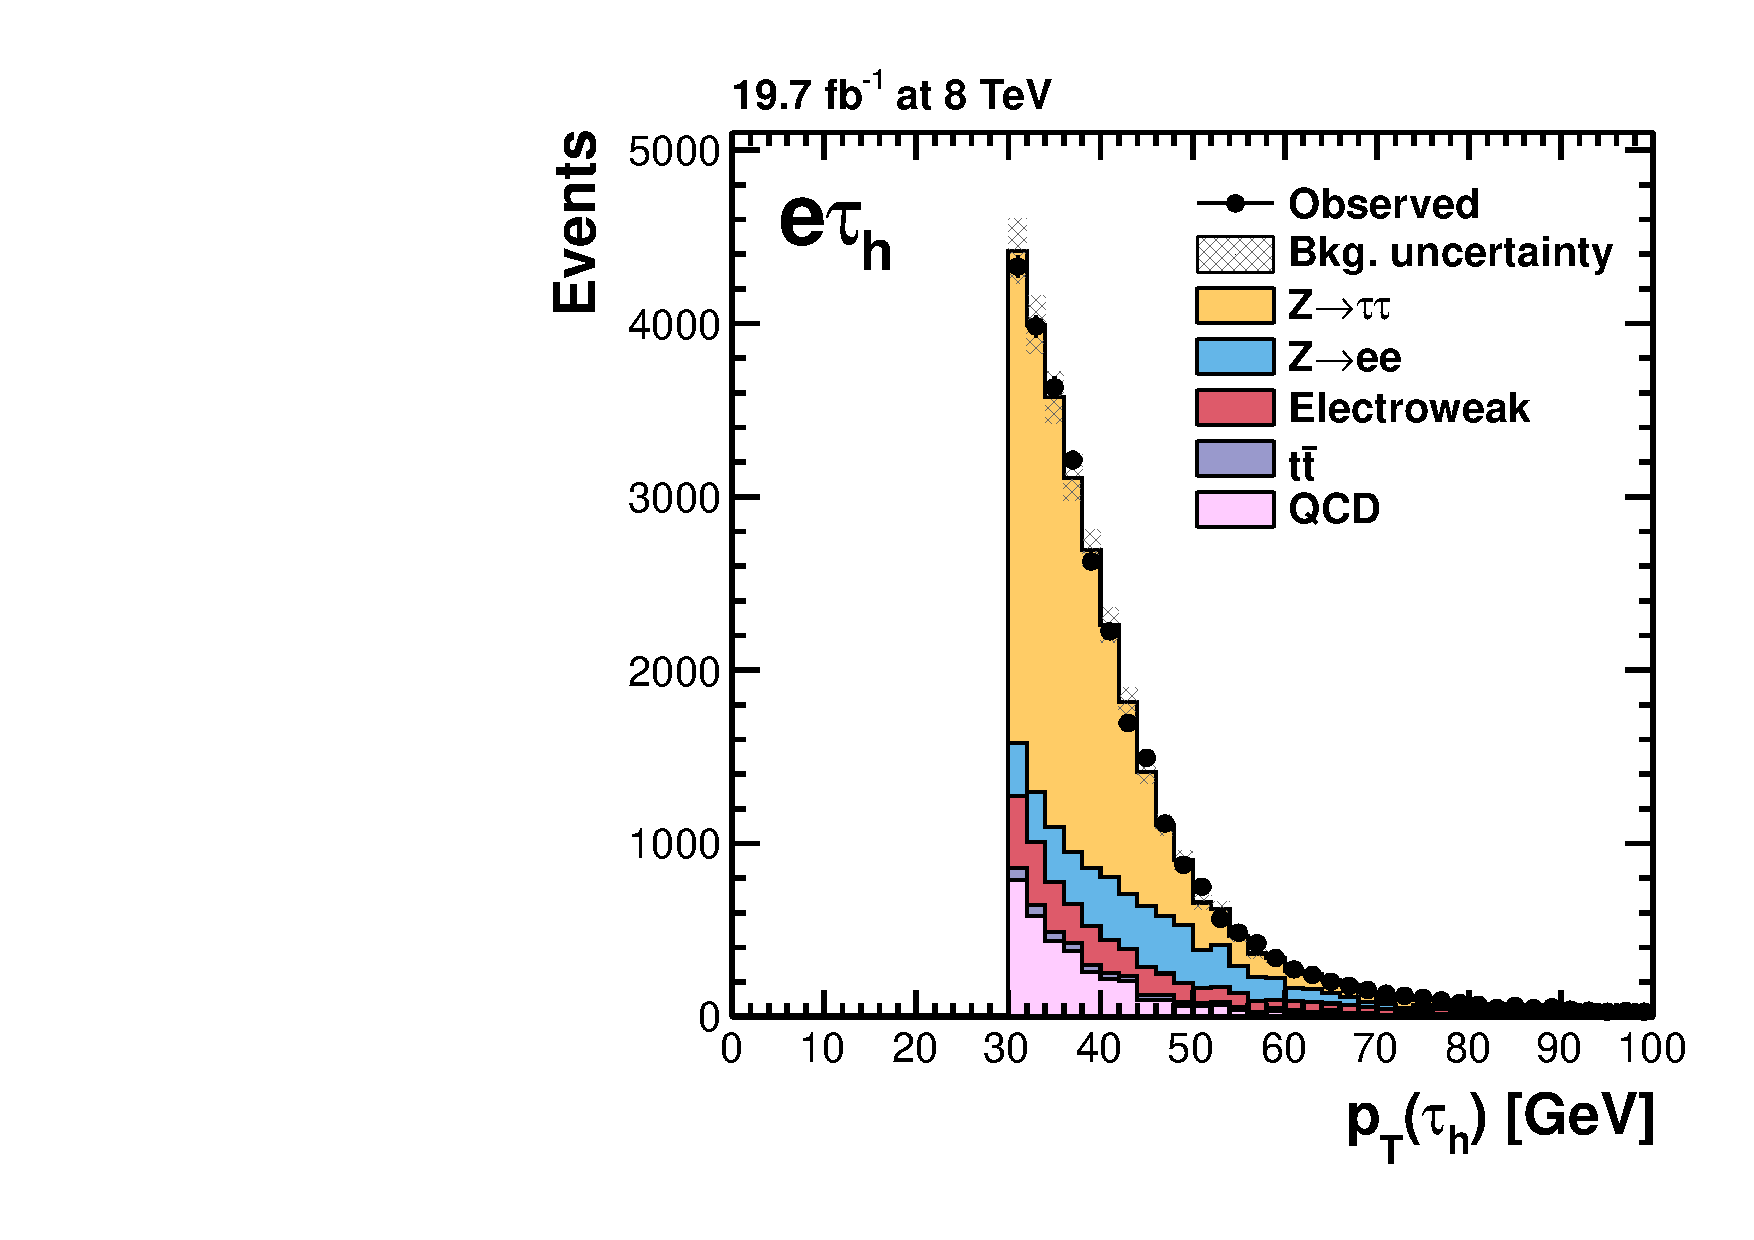
\includegraphics[width=0.5\textwidth]
      {plots/htt-sm/pt_2_inclusive_et_2012.pdf}}
\subfloat[]{
    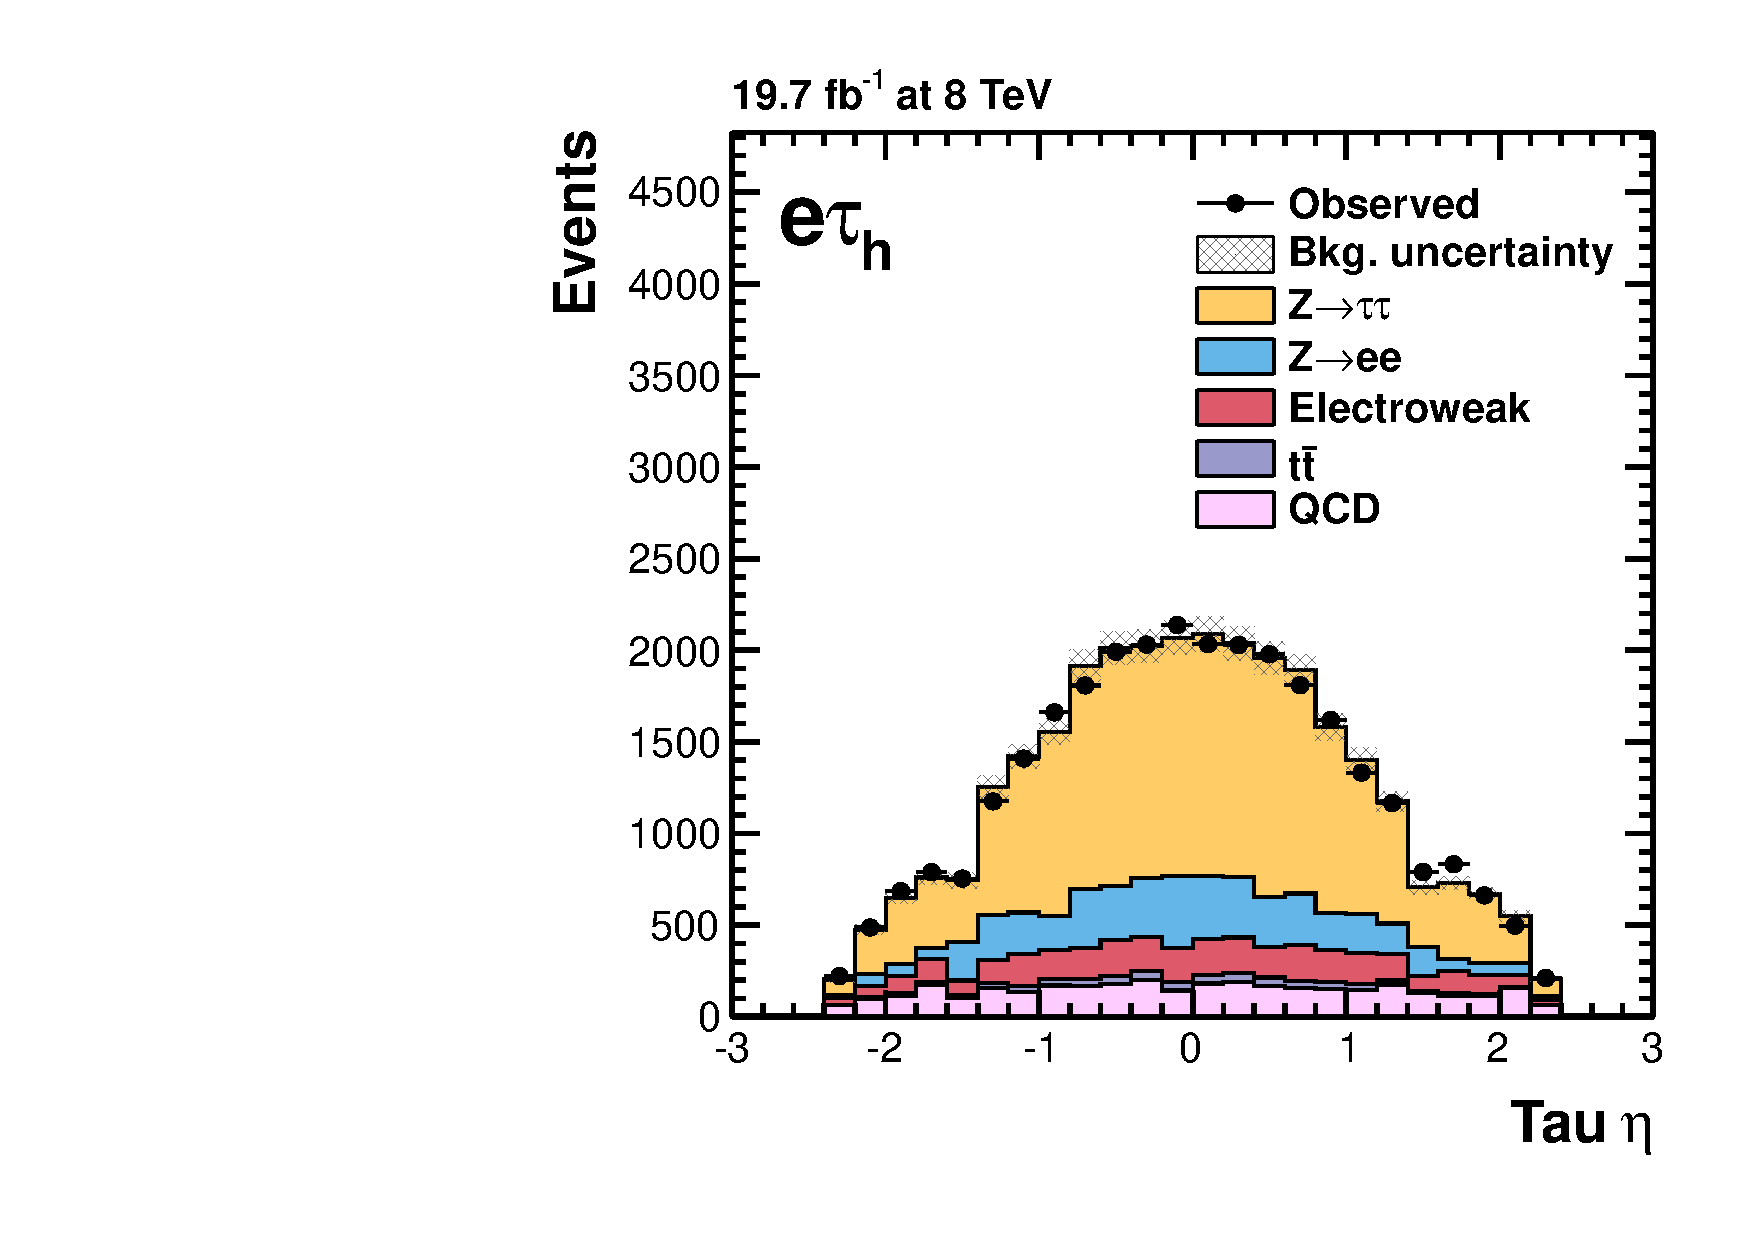
\includegraphics[width=0.5\textwidth] 
      {plots/htt-sm/eta_2_inclusive_et_2012.pdf}} 

\end{center}
\caption{
The $\pt$ and $\eta$ distribution for tau candidates in the $\etau$
channel.
}
\label{fig:etautaus}
\end{figure}

\subsection{Candidate Pair in the $\mutau$ Channel}

Selected events in the $\mutau$ channel require a muon and hadronic tau
candidate. The events are first selected by a trigger algorithm which requires
a muon and tau object. This is done in the same way as for the $\etau$ channel,
where the trigger object at \ac{L1} is a muon and the hadronic tau is
reconstructed at \ac{HLT} level.

In the offline selection the muon is required to have $\pt$ larger than ($17~\GeV$)
$20~\GeV$ in (2011) 2012 data. As for the $\etau$ channel, the higher $\pt$ cut is necessary for the
higher trigger threshold in 2012. In all data taking periods the $\eta$ requirement
on the muon is $|\eta| < 2.1$. The muon is required to pass tight muon ID as
defined in section \ref{sec:muons}. The isolation definition described in 
section \ref{sec:leptonisolation} is
applied with a threshold of $I_{\text{rel}} < 0.1$. Finally, impact parameter cuts on the muon are
applied in exactly the same way as for the electron of the $\etau$ channel.

The hadronic tau has the same ID and isolation definition as described for the $\etau$
channel, with the exception of the anti-electron and anti-muon discriminators.
In the $\mutau$ channel a tight anti-muon discriminator and a loose
anti-electron discriminator are used. 

Similarly to the $\etau$ channel, the muon and hadronic tau are required to be of 
opposite charge, and if more than one such pair exists then the pair with the highest sum $\pt$
is selected. The $\pt$ and $\eta$ distributions of the candidate pair in the
$\mutau$ channel are shown in figure \ref{fig:mutaumuons} for the muon and
\ref{fig:mutautaus} for the tau. 


\begin{figure}[htb]
\begin{center}
\subfloat[]{
    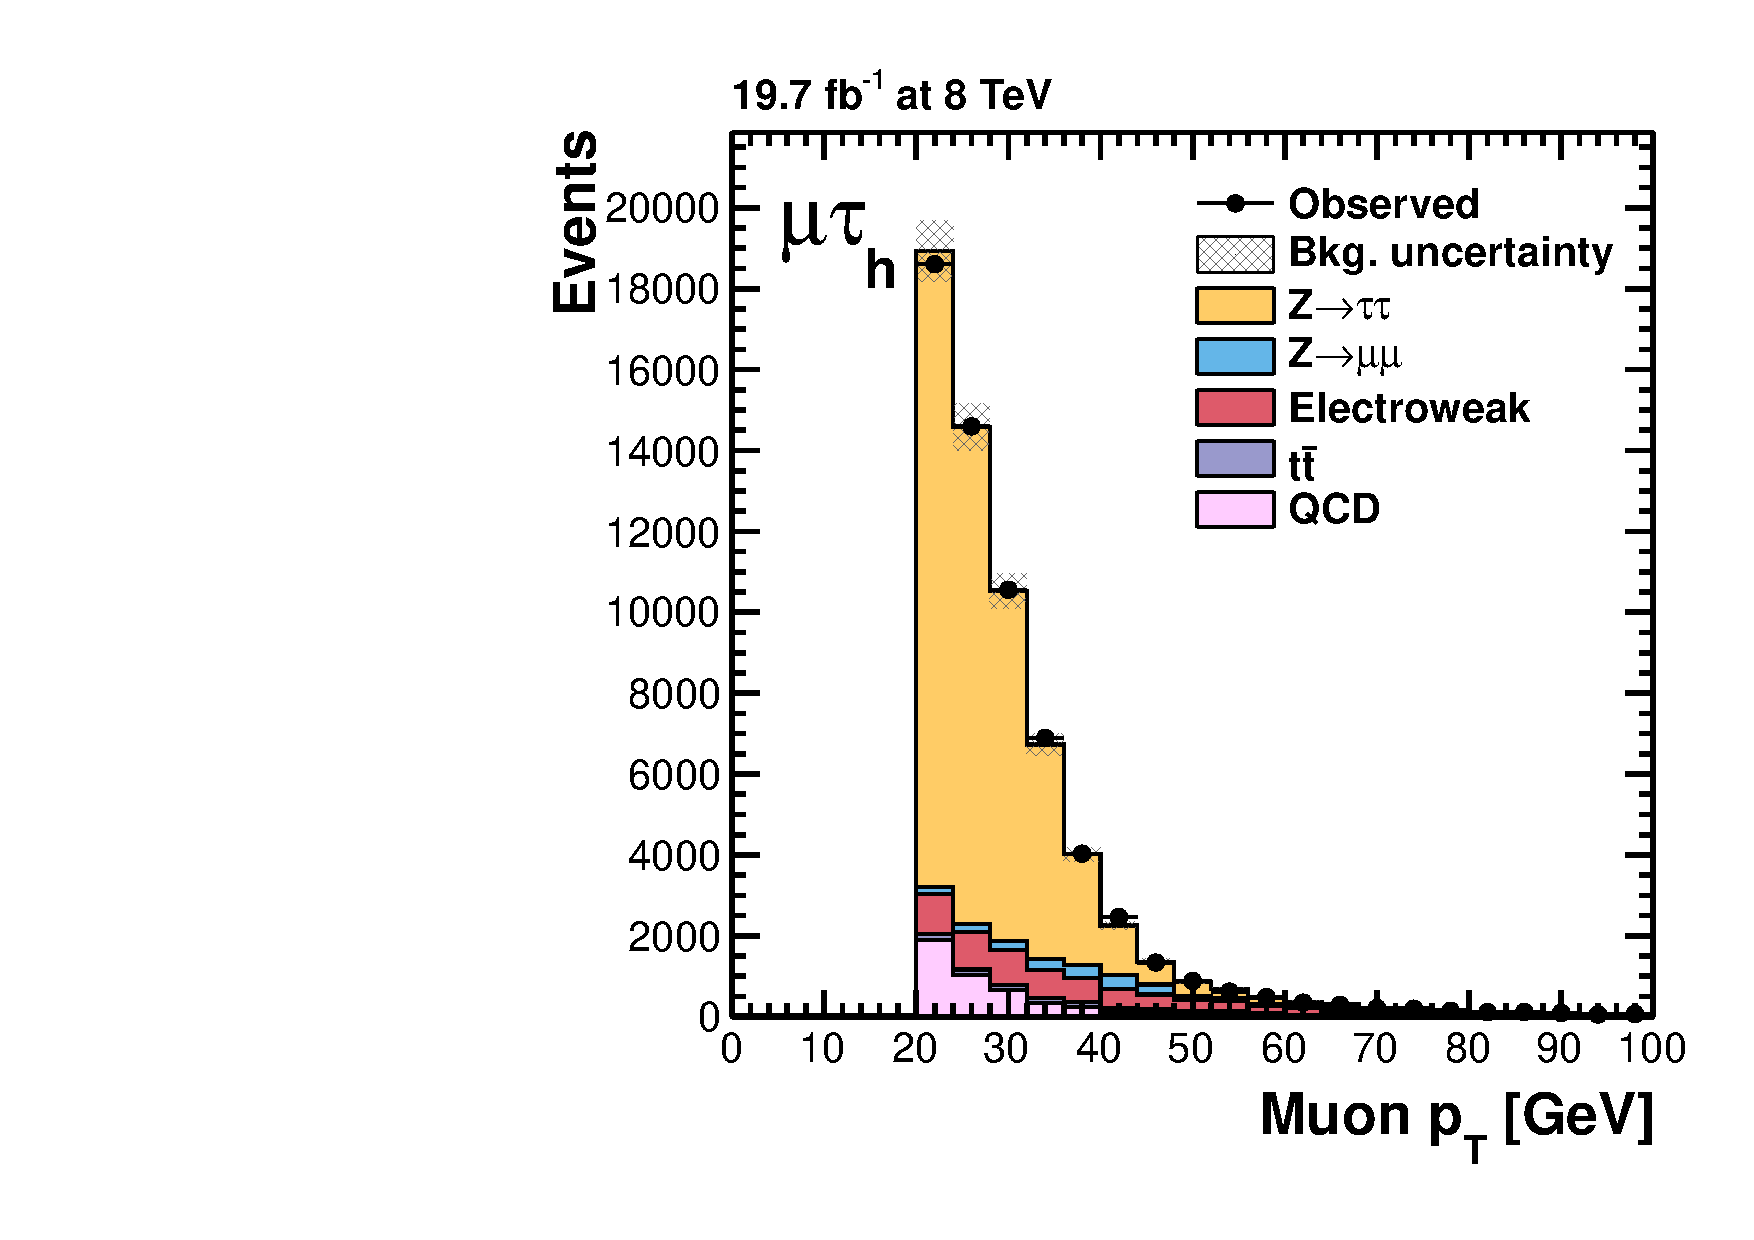
\includegraphics[width=0.5\textwidth]
      {plots/htt-sm/pt_1_inclusive_mt_2012.pdf}}
\subfloat[]{
    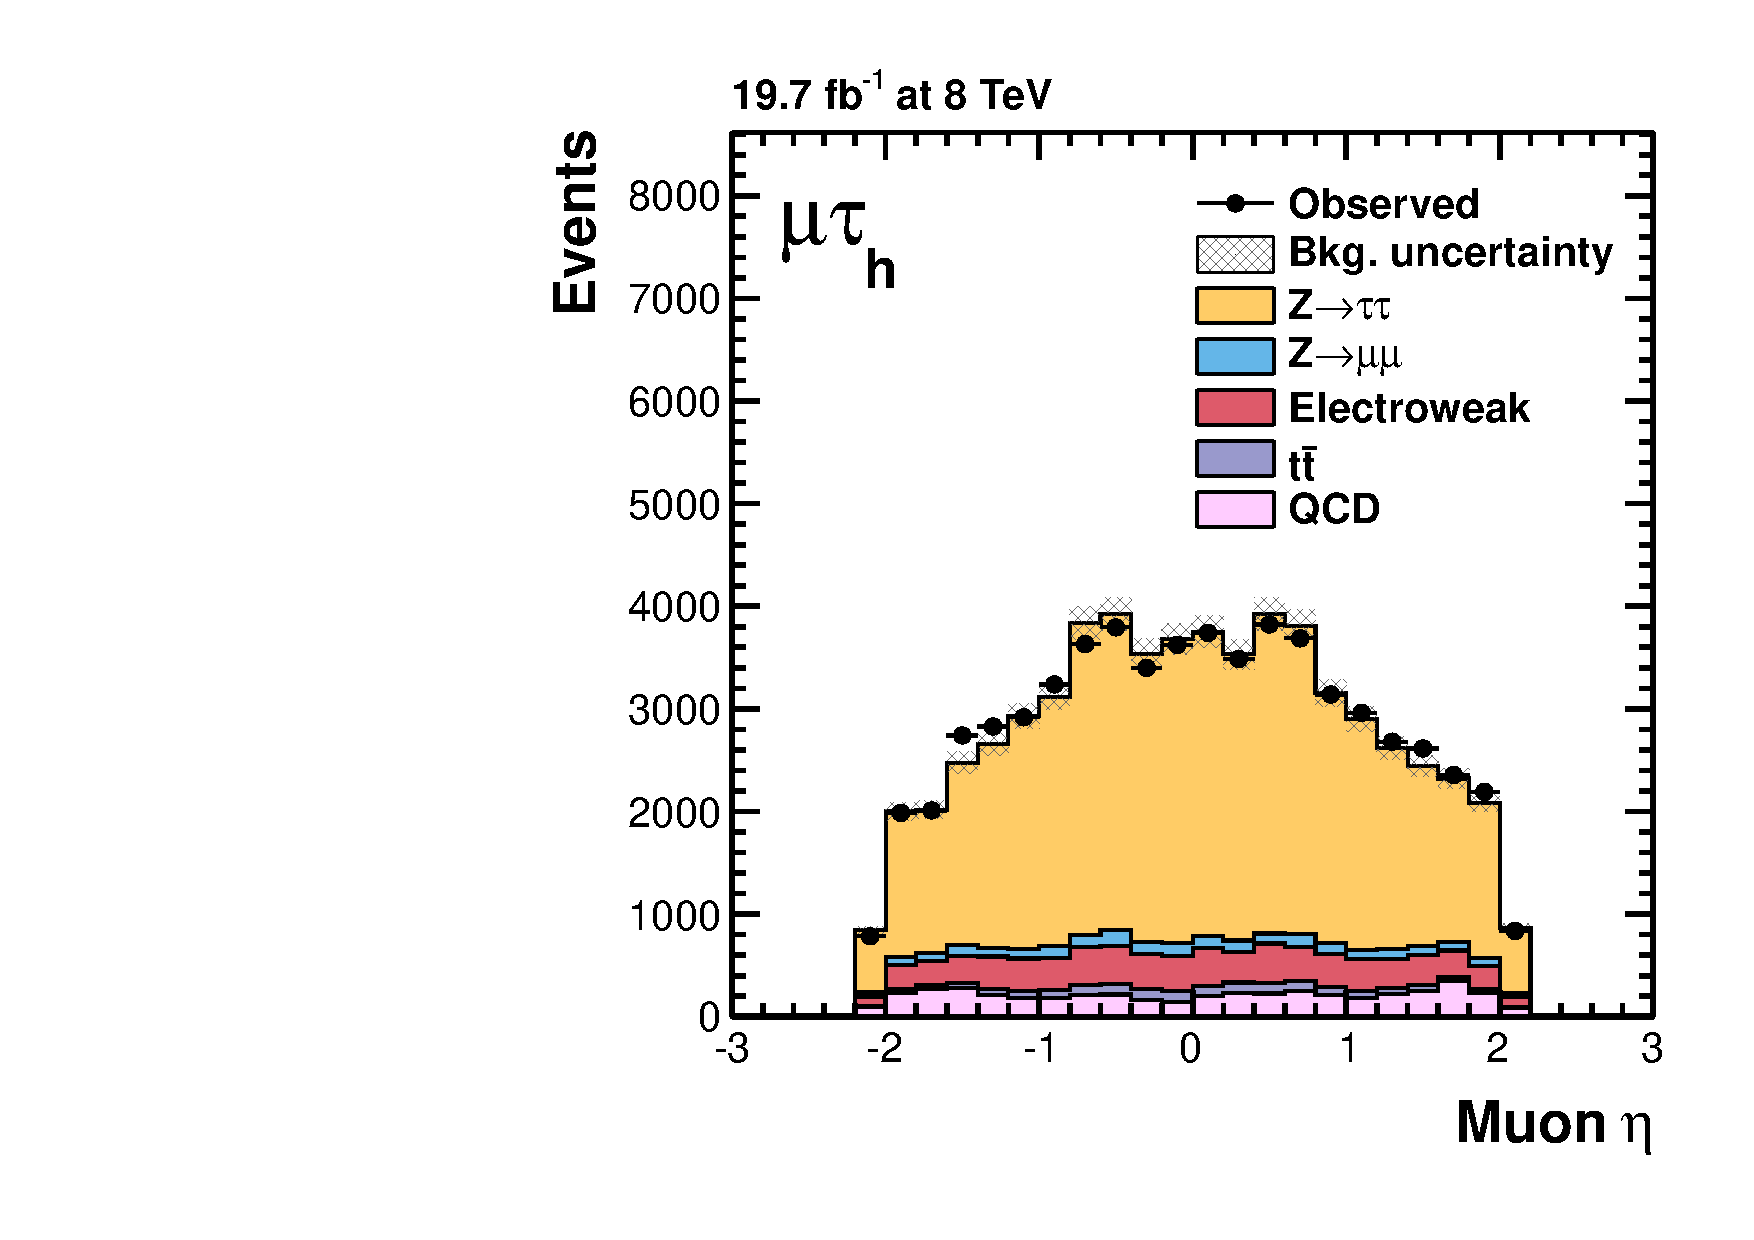
\includegraphics[width=0.5\textwidth] 
      {plots/htt-sm/eta_1_inclusive_mt_2012.pdf}} 

\end{center}
\caption{
The $\pt$ and $\eta$ distribution for muon candidates in the $\mutau$
channel.
}
\label{fig:mutaumuons}
\end{figure}


\begin{figure}[htb]
\begin{center}
\subfloat[]{
    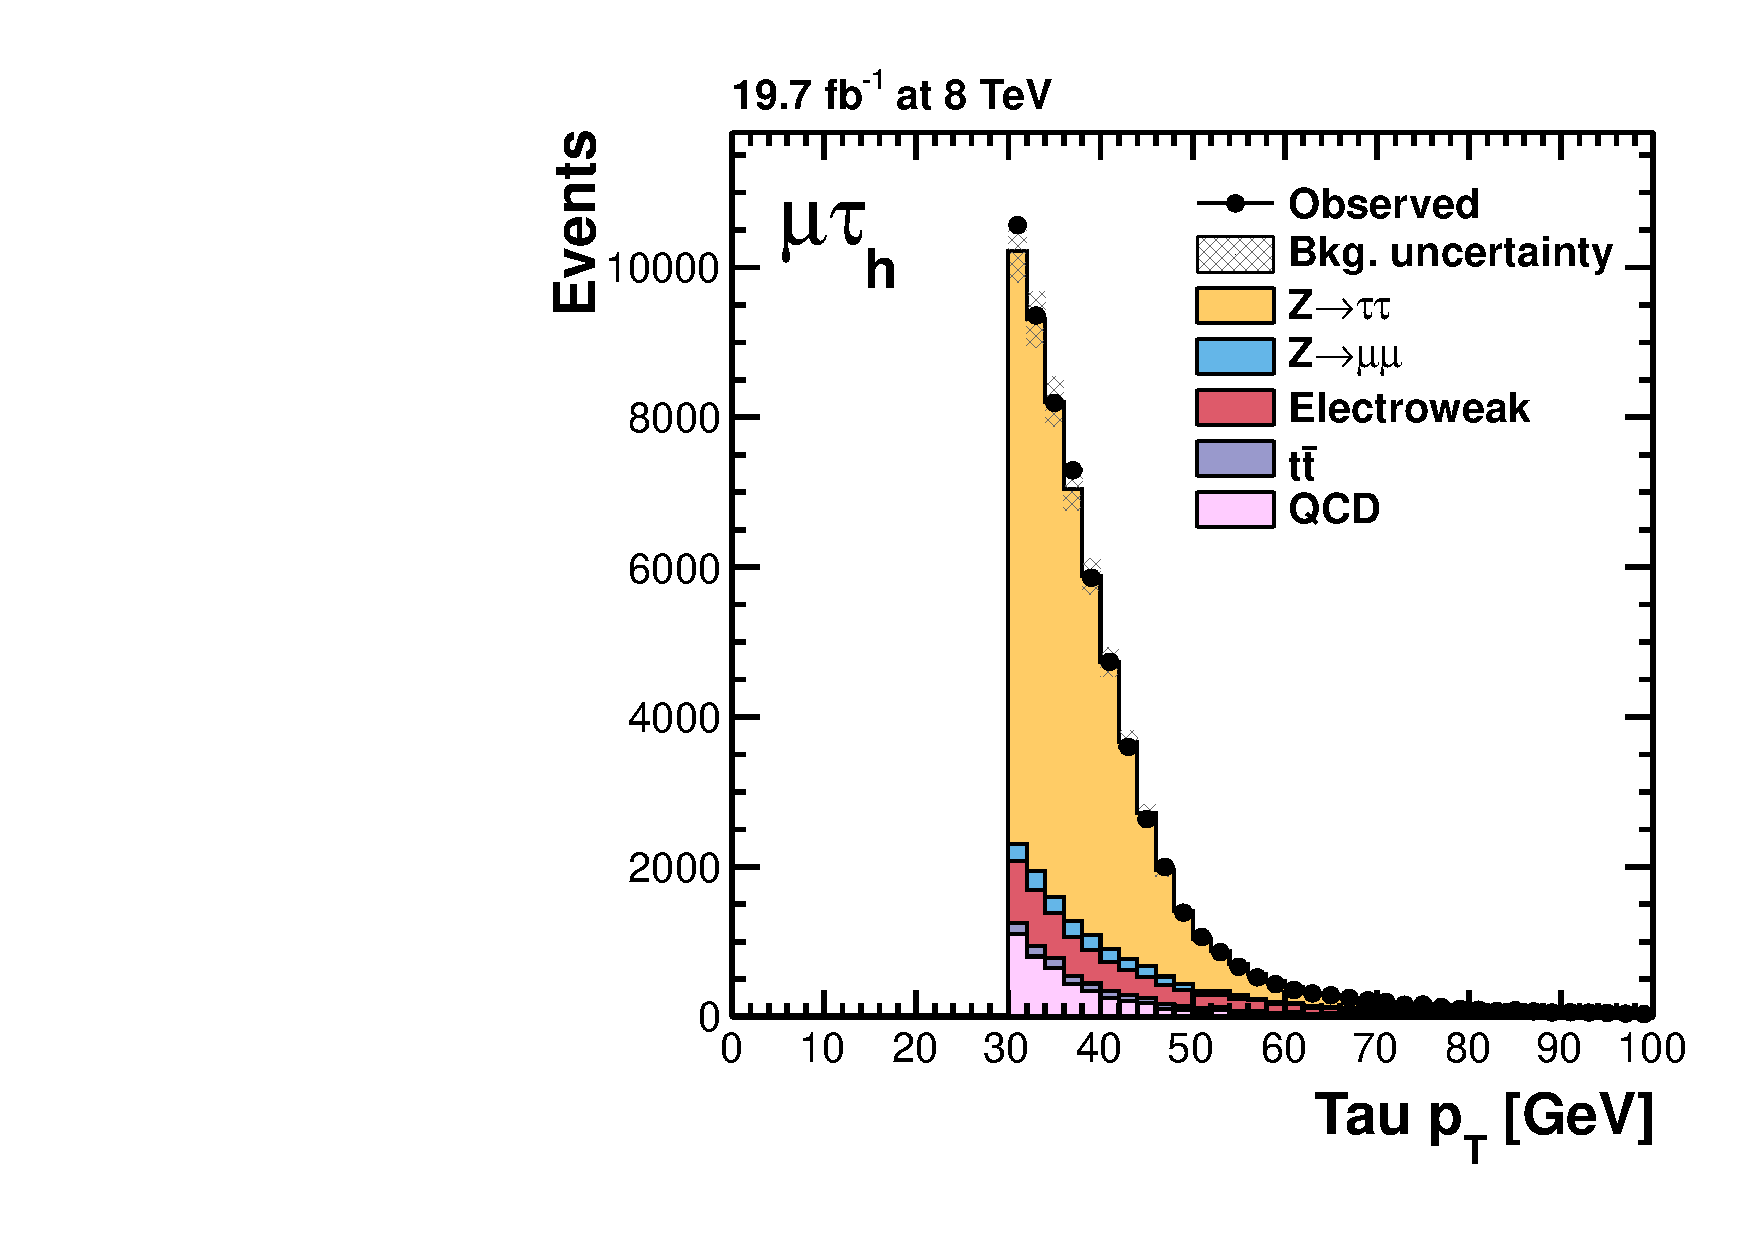
\includegraphics[width=0.5\textwidth]
      {plots/htt-sm/pt_2_inclusive_mt_2012.pdf}}
\subfloat[]{
    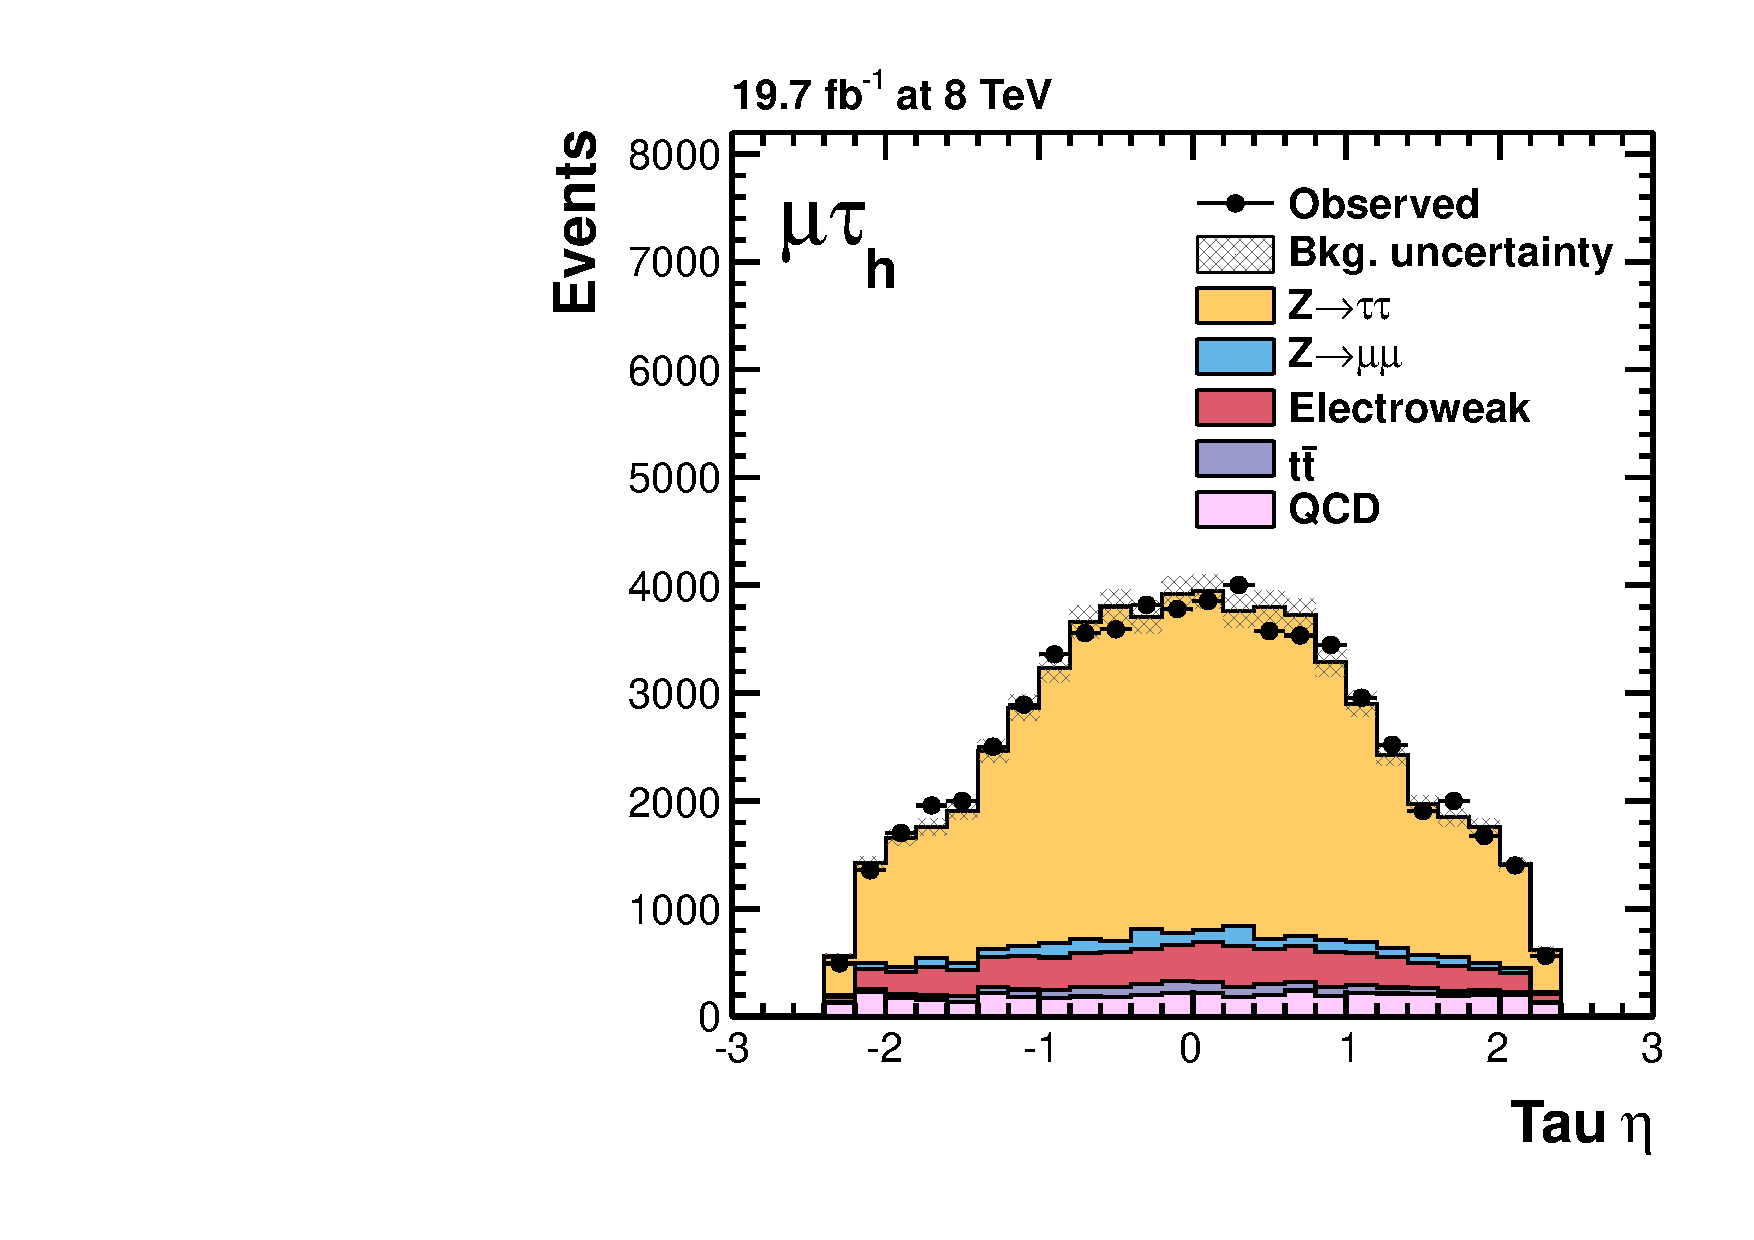
\includegraphics[width=0.5\textwidth] 
      {plots/htt-sm/eta_2_inclusive_mt_2012.pdf}} 

\end{center}
\caption{
The $\pt$ and $\eta$ distribution for tau candidates in the $\mutau$
channel.
}
\label{fig:mutautaus}
\end{figure}

\subsection{Extra lepton vetos}

The contribution of certain backgrounds is reduced by vetoing events with extra
leptons in them. This is also crucial to ensure there is no event overlap
between categories, for example between the $\mutau$ channel and the
$\PW\PH\to\Pgt\Pgt$ analysis in the $\mu\mu\tau_{h}$ final state. In the
$\mutau$ and $\etau$ channels, events are vetoed if they contain an extra muon
or electron respectively, to reduce contribution from $\PZ\to\ell\ell$ in which
the $\tau_{h}$ is a fake from an extra misidentified jet in the event. In these
vetos, the definition of the extra lepton is slightly looser than the lepton ID
used for the candidate pair - with a $\pt$ requirement of $> 15~\GeV$ and
passing loose versions of the ID and isolation. A further veto on all events
containing any additional electron or muon candidate is applied, also with
relaxed selections. 

\subsection{Topological Selection}
\label{sec:topologicalselection}

After selection of the candidate pair, a large background from $\WJets$ remains
in the $\etau$ and $\mutau$ channels, usually with the lepton from the $\PW$ and
a jet faking the hadronic tau. A useful quantity to reduce this background is
the transverse mass between the lepton and the $\MET$:

\begin{equation}
m_{\text{T}}\equiv\sqrt{2\pt^{\ell}\MET(1-\cos(\Delta\phi))},
\end{equation}

where $\pt^{\ell}$ is the $\pt$ of the electron or muon and $\Delta\phi$ is the
difference in azimuthal angle between the lepton and the $\MET$. In real tau
events from $\PZ\to\Pgt\Pgt$ or $\PH\to\Pgt\Pgt$ the neutrinos in the $\Pgt$
decay tend to be produced collinearly with the visible products, whereas in
$\WJets$ events the neutrinos originate from the $\PW$ which has a much higher
mass than the $\Pgt$, and hence the neutrino is more likely to travel in the
opposite direction to the lepton in the transverse plane. Hence $\WJets$ events
have a higher transverse mass than signal events, and so a cut of
$m_{\text{T}}<30\,\GeV$ is found to reduce a large amount of $\WJets$ events
whilst still retaining a good signal efficiency.

Figure \ref{fig:transversemass} shows the distribution of $m_{\text{T}}$ for all
events in the $\mutau$ channel before the $m_{\text{T}}<30\,\GeV$ cut is
applied.

\begin{figure}[htb]
\begin{center}
    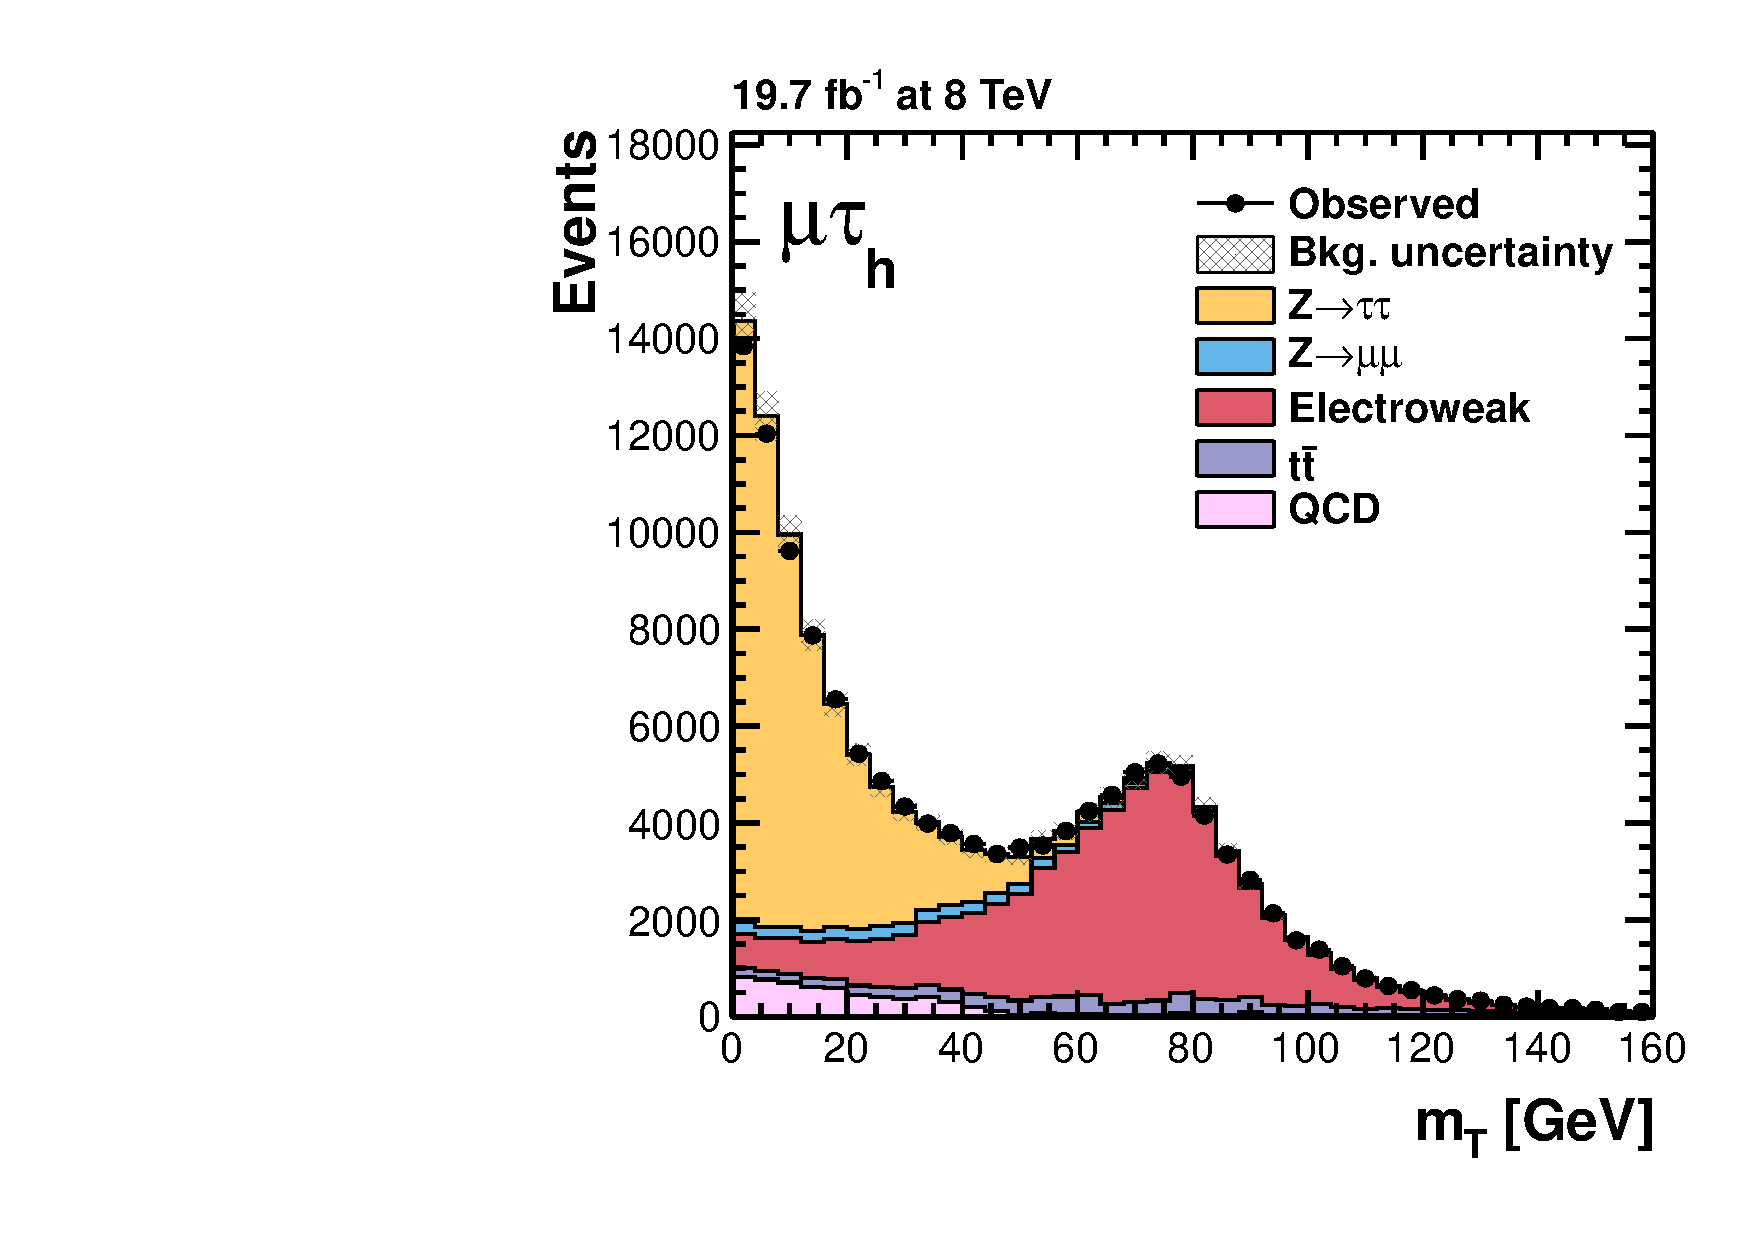
\includegraphics[width=0.5\textwidth]
      {plots/htt-sm/mt_1_inclusive_mt_2012.pdf}

\end{center}
\caption{
 The transverse mass between the muon and the $\MET$ in the $\mutau$ channel.  
}
\label{fig:transversemass}
\end{figure}


\section{Event Categorisation}
\label{sec:eventcategorisation}

The selection as described up until this point is referred to as the
``inclusive'' $\HToTauTau$ selection. 
Events with a good candidate lepton and tau pair are further categorised in
order to group events which are more background-like or signal-like. The
categorisation uses properties consistent with the different production modes of
the Higgs boson as described in section \ref{sec:SMHiggs}. Figure
\ref{fig:smcategories} illustrates these categories for the $\mutau$ and $\etau$
channels.

\begin{figure}[htb]
\begin{center}
    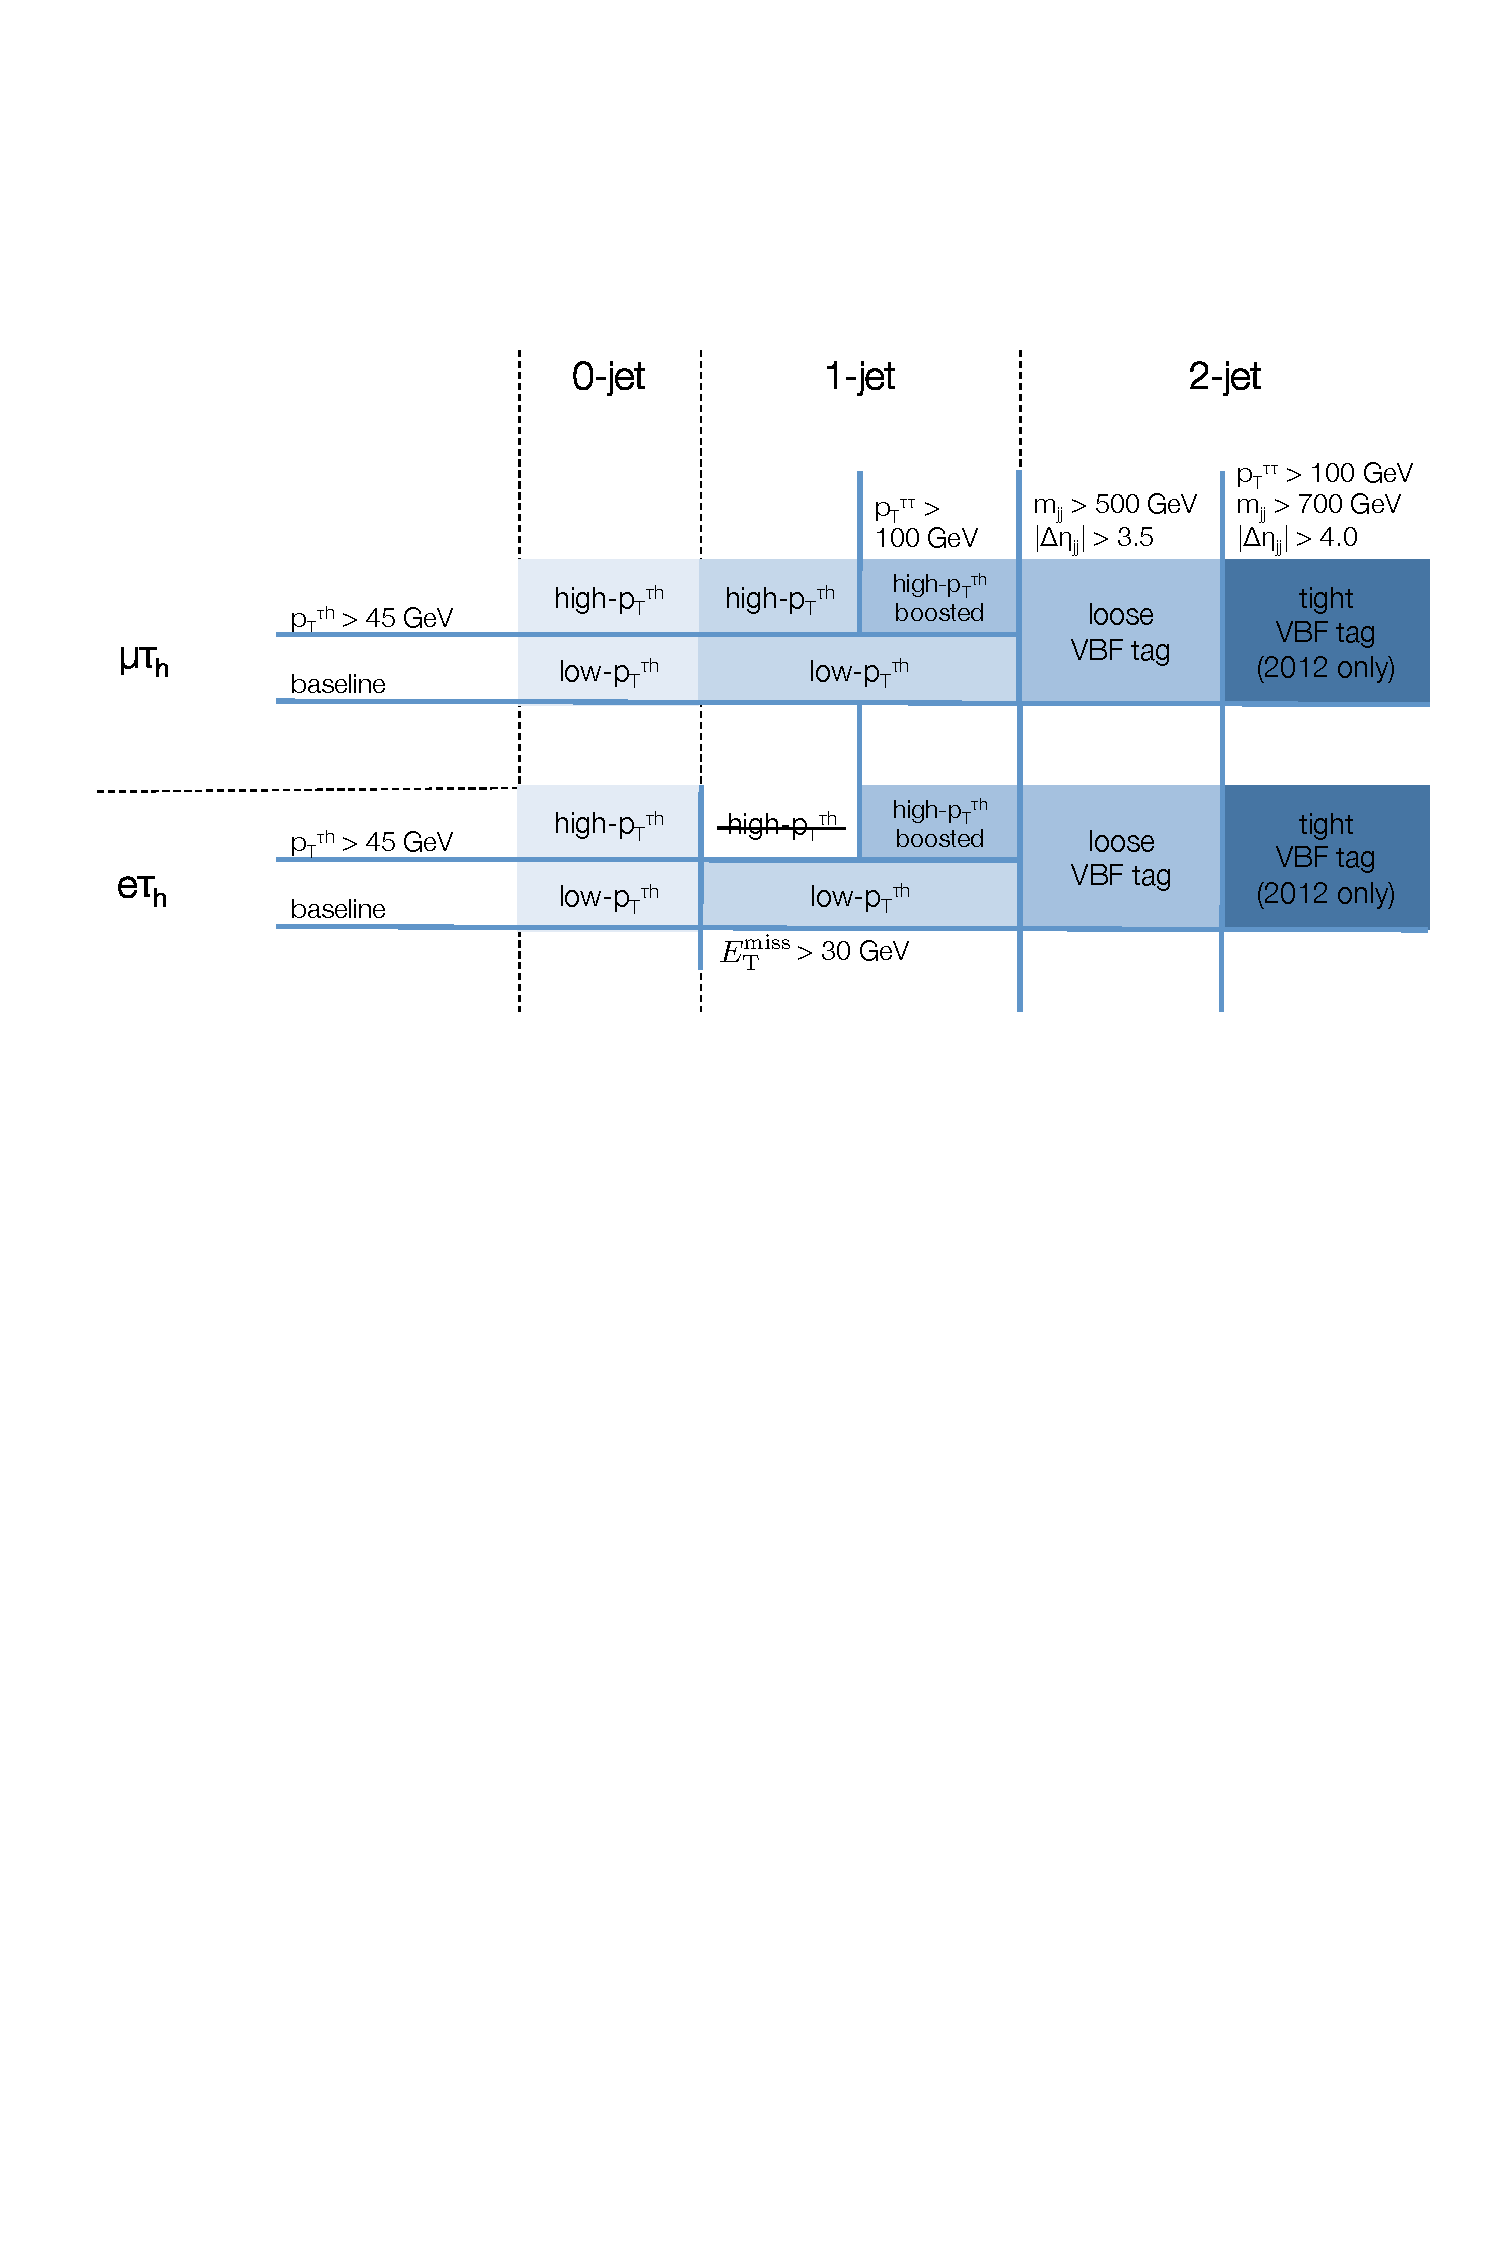
\includegraphics[width=0.8\textwidth]
      {plots/htt-sm/categories_2012.pdf}
\end{center}
\caption{
 Categories used in the $\etau$ and $\mutau$ channels of the \ac{SM}
 $\HToTauTau$ analysis \cite{HIG-13-004}.  
}
\label{fig:smcategories}
\end{figure}

The categorisation separates events which have 0, 1 or $\geq$2 jets with $\pt > 30~\GeV$
and $|\eta| < 4.7$. The jets are required to be separate from the lepton
candidates by $\Delta R > 0.5$. Events which contain a b-tagged jet as described in section
\ref{sec:btag} are vetoed to reduce the contribution of the $\ttbar$ background. 
The 0--jet categories are background dominant, and are included in the final
signal extraction to provide constraints on the backgrounds for the more signal
sensitive categories. The 1--jet categories are sensitive to gluon fusion Higgs
production in association with a jet and \ac{VBF} Higgs production where one jet is
not picked up by the detector. The 2-jet categories are sensitive to
\ac{VBF} Higgs production, and the additional cuts on $m_{jj}$ and $\Delta
\eta_{jj}$ exploit the topology of this process. Events with additional jets in
the $\Delta \eta_{jj}$ gap are vetoed to reduce the \ac{QCD} background.

To improve sensitivity, categories are further separated into more signal-like
and background-like events. The 0--jet and 1--jet categories are separated by
$\Pgth$ $\pt$. The high $\pt^{\Pgth}$ events are more likely to be
consistent with a $\HToTauTau$ event than a $\ZToTauTau$ event due to the higher
mass of the Higgs than the $\PZ$. This also reduces contributions from \ac{QCD}
and $\WJets$ processes, where the jet faking the hadronic tau is likely to be
softer. An additional boosted category is used in 1-jet high $\pt^{\tau_{h}}$
events with a cut on the di-tau $\pt$, defined as:
\begin{equation}
\pt^{\Pgt\Pgt} = |\vec{\pt}^{\Pe/\Pmu} + \vec{\pt}^{\Pgth}+\vecMET|,
\end{equation}
%where $L$ and $L'$ are the electron/muon and $\Pgth$ candidates, 
with the requirement $\pt^{\Pgt\Pgt}>100~\GeV$. The VBF categories are split into VBF
``tight'' and ``loose'' based on tighter or looser $m_{jj}$ and
$\Delta\eta_{jj}$ cuts and the inclusion of the same ditau $\pt$ cut as in the
boosted 1-jet category. The distribution of the $\pt^{\Pgt\Pgt}$ in the
$\mutau$ channel is shown in figure \ref{fig:ditaupt}. 

\begin{figure}[htb]
\begin{center}
    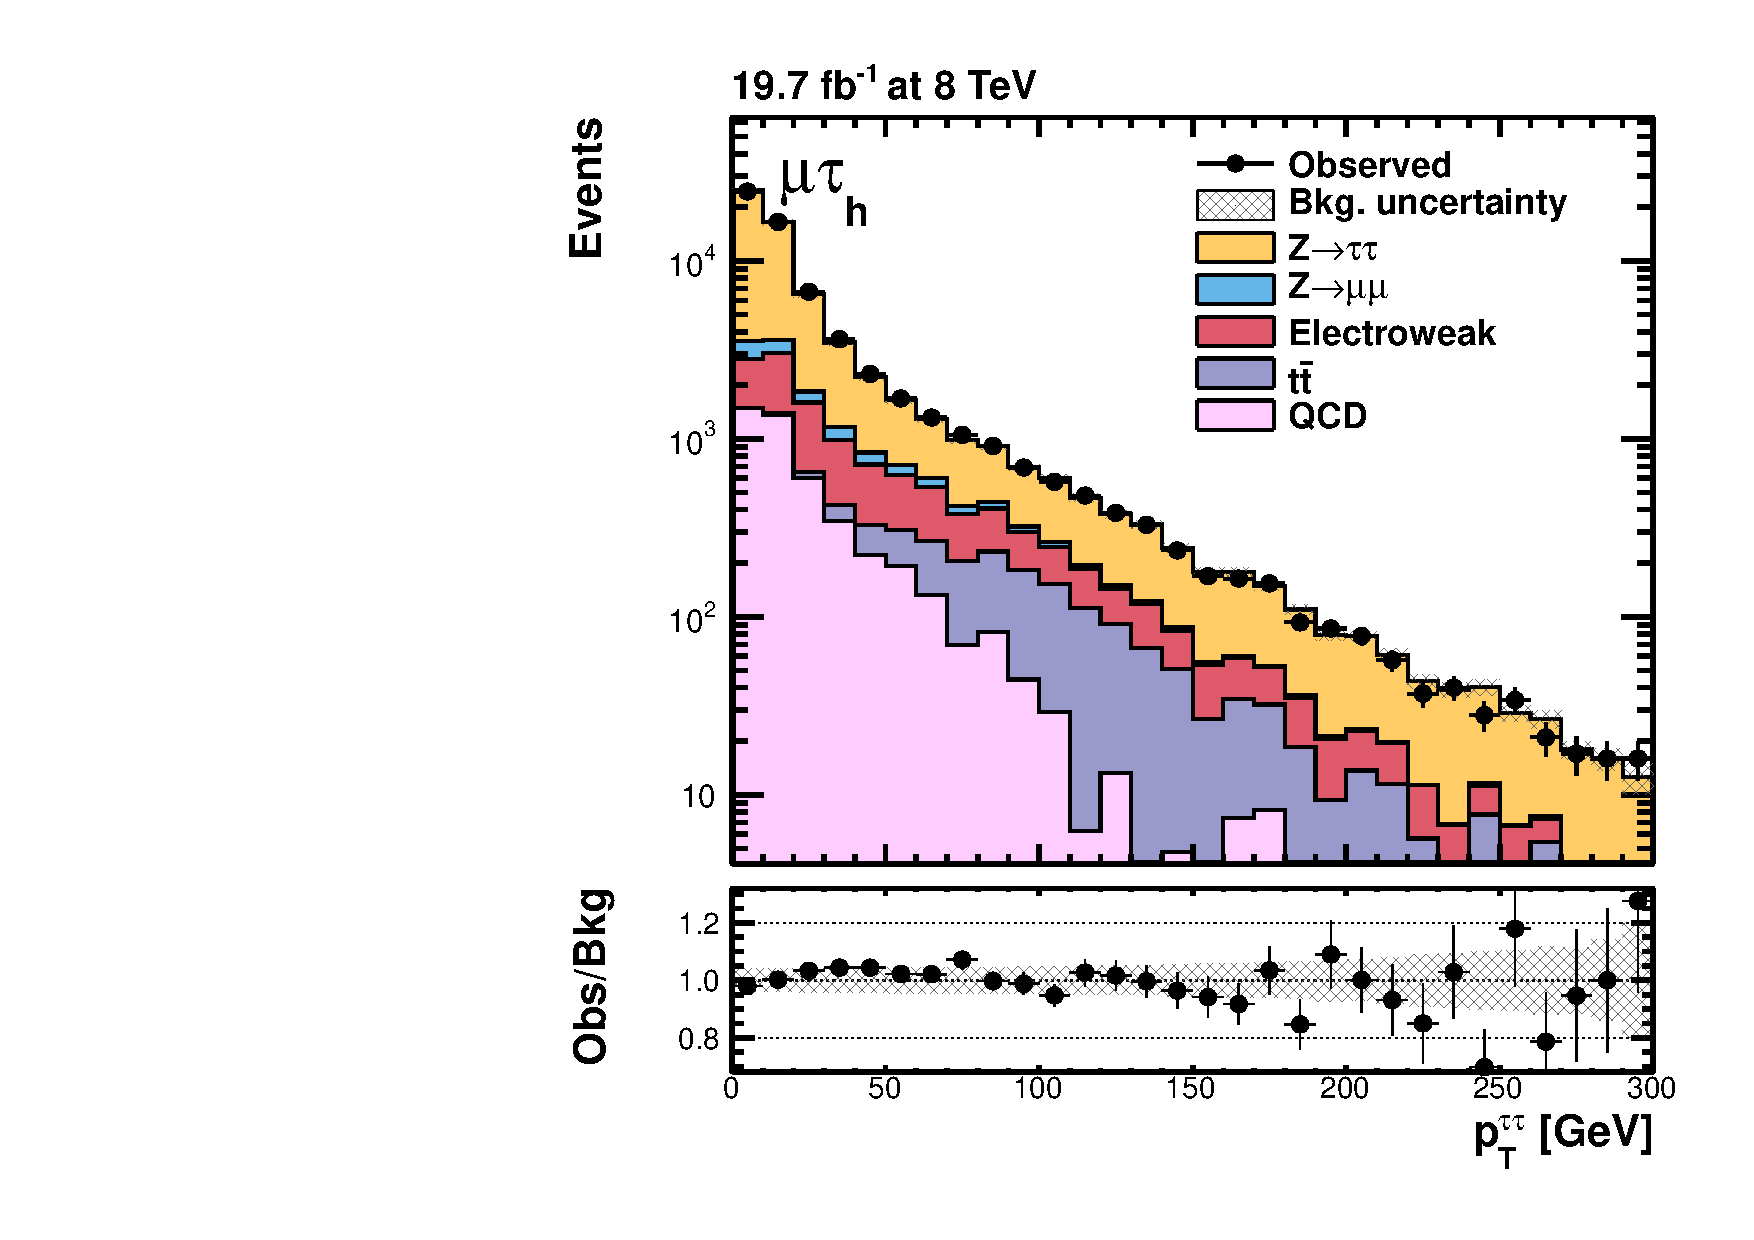
\includegraphics[width=0.5\textwidth]
      {plots/htt-sm/pt_tt_inclusive_mt_2012_log.pdf}
\end{center}
\caption{
 Di-tau $\pt$ in the $\mutau$ channel as used for the separation of events into
 categories. 
}
\label{fig:ditaupt}
\end{figure}

The boosted 1--jet and the VBF tight categories are very 
signal sensitive, and also select events wth the best $m_{\tau\tau}$ resolution.
The VBF tight category is not possible in 2011 data due to the lower statistics,
so the VBF tight and VBF loose categories are merged. 

In the $\etau$ channel, 1--jet categories have an additional cut of $\MET >
30~\GeV$ to reduce the background from $\PZ\to\Pe\Pe$. This cut suppresses the
signal and $\ZToTauTau$ events with low $\pt^{\Pgt\Pgt}$, and as such the 1-jet low
$\pt^{\Pgt\Pgt}$ category is not possible in the $\etau$ channel. 

In all categories in the $\etau$ and $\mutau$ channels, the final discriminating
distribution for signal extraction is the SVFit di-tau mass, as described in
section \ref{sec:svfit}. The method used for signal extraction is described
further in section \ref{sec:signalextraction}.

\section{Datasets and \ac{MC} samples}
\label{sec:dataandMC}

The datasets used in this analysis correspond to all data collected during the 2011 and
2012 running periods of the \ac{LHC}. Samples of background and signal events are produced using several different
\ac{MC} generators. The \textsc{madgraph}~\cite{Alwall:2011uj} matrix element
generator is used for the $\ZJets$, $\WJets$, diboson ($\PW\PW$, $\PZ\PZ$ and
$\PW\PZ$) and $\ttbar$ backgrounds. 
In order to have high enough statistics to evaluate the
backgrounds in categories with varying jet multiplicities, extra samples are
generated with fixed jet multiplicities up to 4. These are combined with
inclusive samples using the expected ratio to retain the correct cross-section
ratios between different jet multiplicities. 

The single top samples are generated using
\textsc{powheg}~\cite{Frixione:2007vw,Alioli:2010xd,Alioli:2010xa}, as are the
signal samples for gluon-fusion and \ac{VBF} at \ac{NLO} precision. Signal
samples for production in association with a vector boson are generated using
\textsc{pythia}~\cite{Sjostrand:2006za} at \ac{LO} precision. In all
samples, \textsc{pythia} is used for parton showering and hadronisation and
\textsc{tauola}~\cite{TAUOLA} is used for tau decays. Minimum bias events
generated by \textsc{pythia} are added to all generated Monte Carlo samples
to simulate additional proton-proton interactions, and then the events are
weighted to match the pile-up distribution observed in data. 

For the signal, \ac{MC} samples are produced in $5~\GeV$ steps between
$m_{\PH}=90~\GeV$ and $m_{\PH}=145~\GeV$. The cross-sections and branching ratios 
are taken from the \ac{LHCHXSWG}
\cite{LHCHiggsCrossSectionWorkingGroup:2011ti,Dittmaier:2012vm,Heinemeyer:2013tqa}.
The full set of simulated processes, the \ac{MC} generators used and the
corresponding cross-sections can be found in table \ref{tab:datasetsandMC}.

\begin{table}[tbh]
\begin{tabular}{|l|c|c|c|}
\hline
Process & \ac{MC} Generator & \multicolumn{2}{|c|}{Cross Section [$\picobarn$]} \\
\cline{3-4}
&  & 7 \TeV & 8 \TeV \\
\hline
\hline
$\PW\to L\nu$ & \textsc{madgraph} & $31314$  & $36257$ \\
$\Pqt\Paqt$ & \textsc{madgraph}   & $164.4$   & $249.5$ \\
$\PZ\to LL$ & \textsc{madgraph}                      & $3048$    & $3504$ \\
$\PW\PZ\to \Pq\Pq'LL$ & \textsc{madgraph}          & $1.8$     & $2.2$ \\
$\PW\PZ\to L\Pnu LL$ & \textsc{madgraph}            & $0.9$     & $1.1$ \\
$\PZ\PZ\to LLLL$ & \textsc{madgraph}           & $0.06$    & $0.18$ \\
$\PZ\PZ\to LL\Pq\Pq$ & \textsc{madgraph}           & $0.8$     & $2.5$ \\
$\PZ\PZ\to LL\Pnu\Pnu$ & \textsc{madgraph}         & $0.3$     & $0.7$ \\
Single-top ($\Pqt\PW$ channel) & \textsc{powheg}            & $15.7$    & $22.2$ \\
\hline
SM $\Pg\Pg\PH(\Pgt\Pgt)$ & \textsc{powheg} & $0.96$ & $1.22$ \\
SM $\Pq\Pq\PH(\Pgt\Pgt)$ & \textsc{powheg} & $0.077$ & $0.010$ \\
SM $\PZ\PH(\Pgt\Pgt)$+$\PW\PH(\Pgt\Pgt)$+$\Pqt\Paqt\PH(\Pgt\Pgt)$ &
\textsc{pythia} & $0.063$ & $0.079$ \\
\hline
\end{tabular}
\caption{
Summary of the background and signal processes used in the $\HToTauTau$ analysis along with the
\ac{MC} generator and cross-section for the process for $\sqrt{s}$ = $7~\TeV$ or $8~\TeV$. 
The notation $L$ indicates a leptonic decay into $\Pe$, $\Pmu$ or
$\Pgt$, and $q$ indicates a quark. For the $\PW$, $\PZ$ and diboson backgrounds
samples are produced for jet multiplicities of 0, 1, 2, 3 and 4. The
cross-sections listed for the signal process are for $m_{\PH}=125~\GeV$.
}
\label{tab:datasetsandMC}
\end{table}

\section{Background Estimation}
\label{sec:backgrounds}

There are many backgrounds to $\HToTauTau$. Where possible, data driven methods
are used to minimise systematic uncertainty related to the modelling in the
\ac{MC}. It is essential to accurately estimate both the shape and the overall
yield of each background, and the following sections describe how this is done
individually for each source of background.

\subsection{Drell-Yan $\PZ \to\Pgt\Pgt$}
\label{sec:backgroundEstimation_Ztautau}

The $\PZ \to \Pgt\Pgt$ component is the largest and is usually referred to as ``irreducible", due to its final
state involving two real taus which only differ from the $\PH \to \Pgt\Pgt$ signal by
having an invariant mass closer to $m_{\PZ}$ than $m_{\PH}$.
The contribution from $\ZToTauTau$ in each category is estimated using an
``embedded'' sample. In this process a sample of $\PZ\to\Pmu\Pmu$ events in data are
collected and the muons replaced with simulated taus. These muons are required
to pass \ac{PF} identification and loose isolation and be of opposite charge.
The simulated taus are assigned the 4-momenta of the muons, and all other
quantities such as jets, $\MET$ and tau isolation are re-computed. The taus
are simulated using \textsc{tauola}. 
The advantage of this method is that the majority of event objects
are taken from data, and hence the systematic uncertainties related to $\MET$
and jet reconstruction are much smaller. 

To estimate the normalisation of the background in each category, 
the $\ZToTauTau$ \ac{MC} sample is used to estimate 
the inclusive yield of this background without the topological $m_{\text{T}}$
cut. Then the yield in each category is estimated by scaling this inclusive yield by the efficiency for 
inclusive events to pass the category selection plus $m_{\text{T}}$ cut, which is estimated using the
embedded sample. The shape is then taken from the embedded sample within the
category selection.

%To account for the known contamination of $t \bar{t}$ events in the embedded
%samples, the embedded $t \bar{t}$ samples described in
%section~\ref{sec:datasets_and_MonteCarloSamples} are used to evaluate the
%expected contribution from such events, and then this is directly subtracted
%from the $\PZ \to\Pgt\Pgt$ contribution.

\subsection{$\PZ\to\ell\ell$}
\label{sec:backgroundEstimation_Zll}

The $\PZ\to\ell\ell$ background results when one lepton provides the electron or
muon and either the other lepton or an associated jet fakes the hadronic tau. This
background is much smaller than $\ZToTauTau$ but especially important in the
$\etau$ channel where electrons have a $3$-$4\%$ probability to pass the
anti-electron discrimination in the tau ID. Both yield and shape of this
background are taken from simulation.

\subsection{$\WJets$}
\label{sec:backgroundEstimation_WplusJets}

$\WJets$ has already been mentioned in section \ref{sec:topologicalselection},
and is a background in this analysis where there is a real electron or
muon from the W and one of the associated jets fakes a hadronic tau. This
background is largely reduced by the $m_{\text{T}}< 30~\GeV$ cut. 
To estimate the remaining contribution the
events with $m_{\text{T}}> 70~\GeV$ are used, which are dominated by $\WJets$ 
events as can be seen in figure \ref{fig:transversemass}. 
This is used to estimate the sideband normalisation of the $\WJets$, by
subtracting all other backgrounds from data and taking the rest to be $\PW$.
An extrapolation factor from  $m_{\text{T}} > 70~\GeV$ to $m_{\text{T}}< 30~\GeV$, 
is then calculated from MC and scales the sideband normalisation.

The shape of the $\WJets$ is taken from MC in each category. Due to the low number of
events passing the VBF categories, the $m_{jj}$ and $|\Delta\eta_{jj}|$
conditions are relaxed in both calculating the extrapolation factor and
obtaining the shape.

\subsection{QCD}
\label{sec:backgroundEstimation_QCD}

QCD background occurs when both the lepton and the tau are misidentified jets, and is estimated 
entirely from data. It is expected that the contribution of events with a
candidate pair in which the pair have opposite or the same
charges/signs is roughly the same in QCD. Thus the same
sign data is used with all other backgrounds subtracted, to predict the rate of
QCD in the opposite sign events in our signal region. 
For the background subtraction, the $\WJets$ is 
estimated as described in the previous section simply switching opposite sign
events for same sign, and all other background
contributions are estimated from \ac{MC}. The rates of opposite sign to same
sign QCD events are not quite exactly the same, and an extrapolation factor of
1.06 is applied to correct for this. This factor is measured using data with the 
electron/muon isolation inverted to give a pure QCD sample. 

The same sign data is used in this way for extracting the norm in all of the
0--jet and 1--jet
categories, with the exception of 1--jet high-$\pT^{\Pgth}$ boosted.
Due to the low statistics in the 1--jet high-$\pT^{\Pgth}$ boosted and in the VBF
categories, it is necessary to define another
sideband from which to extract the QCD estimate. This is done by inverting the
electron/muon isolation to $0.2 < I_{\text{rel}} < 0.5$ in same-sign events. 
The high purity for QCD multijet events in anti-isolated same sign data makes 
it unnecessary to subtract other backgrounds, which are negligible. 
The inclusive same-sign data yield is taken from the normal 
isolation region, and scaled by the efficiency to go from the inclusive to the 
category selection as estimated in the anti-isolated data. 

In the 0--jet low-$\pT^{\Pgth}$ category the shape is taken from the normal
isolation same-sign data with other backgrounds subtracted. In all other
categories the anti-isolated data is used for the shape. In the 1--jet
high-$\pT^{\Pgth}$ boosted and tight VBF-tag categories the isolation on the
$\Pgt_{had}$ is also loosened to obtain a sufficiently smooth shape.  

\subsection{$\ttbar$}
\label{sec:backgroundEstimation_TT}

For the $t \bar{t}$ both shape and normalisation are taken from MC. Both are checked
against data by defining a control region which is at least 90$\%$ pure in
$t \bar{t}$. This is done using the $\emu$ channel, which has a much higher
quantity of $\ttbar$ than $\etau$ and $\mutau$. The control region is used to
derive a scale factor to the \ac{MC} normalisation. This control region will be
discussed further in chapter \ref{chap:Hhh} in the context of an analysis which
much larger contributions from $\ttbar$ background.  

\subsection{Diboson and single top}
Both the normalisation and shapes of these backgrounds are estimated using MC.
The contributions from these backgrounds are much smaller than the others.

\section{Data/MC Correction Factors}
\label{sec:datamcfactors}

Whilst data-driven methods are used wherever possible, \ac{MC} is still
relied on in predicting expected shapes and yields of signal and some of the
backgrounds, as discussed in the previous section.
As such is it important that the \ac{MC} is corrected for
any effects which are known to be imperfectly modeled. Many of these corrections
are derived by studying the agreement between \ac{MC} and data in dedicated
samples or control regions.

\subsection{ID, isolation and trigger efficiencies}
\label{sec:idisotrigger}

For ID, isolation and trigger efficiencies of the candidate electron/muon 
and tau in the analysis, the \ac{MC} is corrected for measured differences in 
the efficiency of the selection in \ac{MC} compared with data.

This section documents measurements of these efficiences for the electron/muon 
of the $\etau$ and $\mutau$ channels. This is done using a ``tag and probe"
method \cite{Khachatryan:2010xn}.
The method makes use of a well known resonance decaying
into a light lepton pair, in this case $\PZ\to\Pe\Pe$ or $\PZ\to\Pmu\Pmu$, 
in which one the light leptons is assigned as the `tag' and one is the `probe'. 
The tag is constrained by a very tight selection such that it is known with near 
certainty to be a real electron/muon. The probe is subject to a looser selection, 
but only tag/probe pairs with an invariant mass close to the $\PZ$ mass are used. 
This ensures that the probe is also a true electron/muon with high probability. 
Then the probe can be subjected to further cuts or constraints to measure the 
efficiency of such a selection to select real leptons.

The invariant mass distributions of the tag and probe events are used to extract
the different selection efficiencies. A simultaneous fit of the lepton pair mass
shapes is performed for events with a passing and failing probe, 
and the ratio of the integral of the fitted $\PZ$ signal 
in the pass and fail distributions is used to extract the efficiency. To account for any background
to the real $\PZ$ events, signal and background are both accounted for
separately in the fit. An example of such a fit can be seen in figure
\ref{fig:tandp}.

The electron/muon ID efficiency is measured with a reconstructed
electron/muon as the probe, subject only to $\pt$ and $\eta$ cuts. 
Then the electron/muon isolation efficiency is measured
with a probe which already fulfils the full ID selection criteria. 
The efficiencies for combined ID and isolation are shown in Figures
\ref{fig:electronIdIso} and \ref{fig:muonIdIso}, measured in the complete 2012
dataset and \ac{MC}, as a function of the lepton $\eta$ and $\pt$.
The scale factor which is used in the analysis to correct the \ac{MC} is given by the ratio of the
measured efficiency in data (black) and MC (red/blue), and is evaluated separately in
selected $\pt$ and $\eta$ bins.

\begin{figure}[htb]
\subfloat[]{
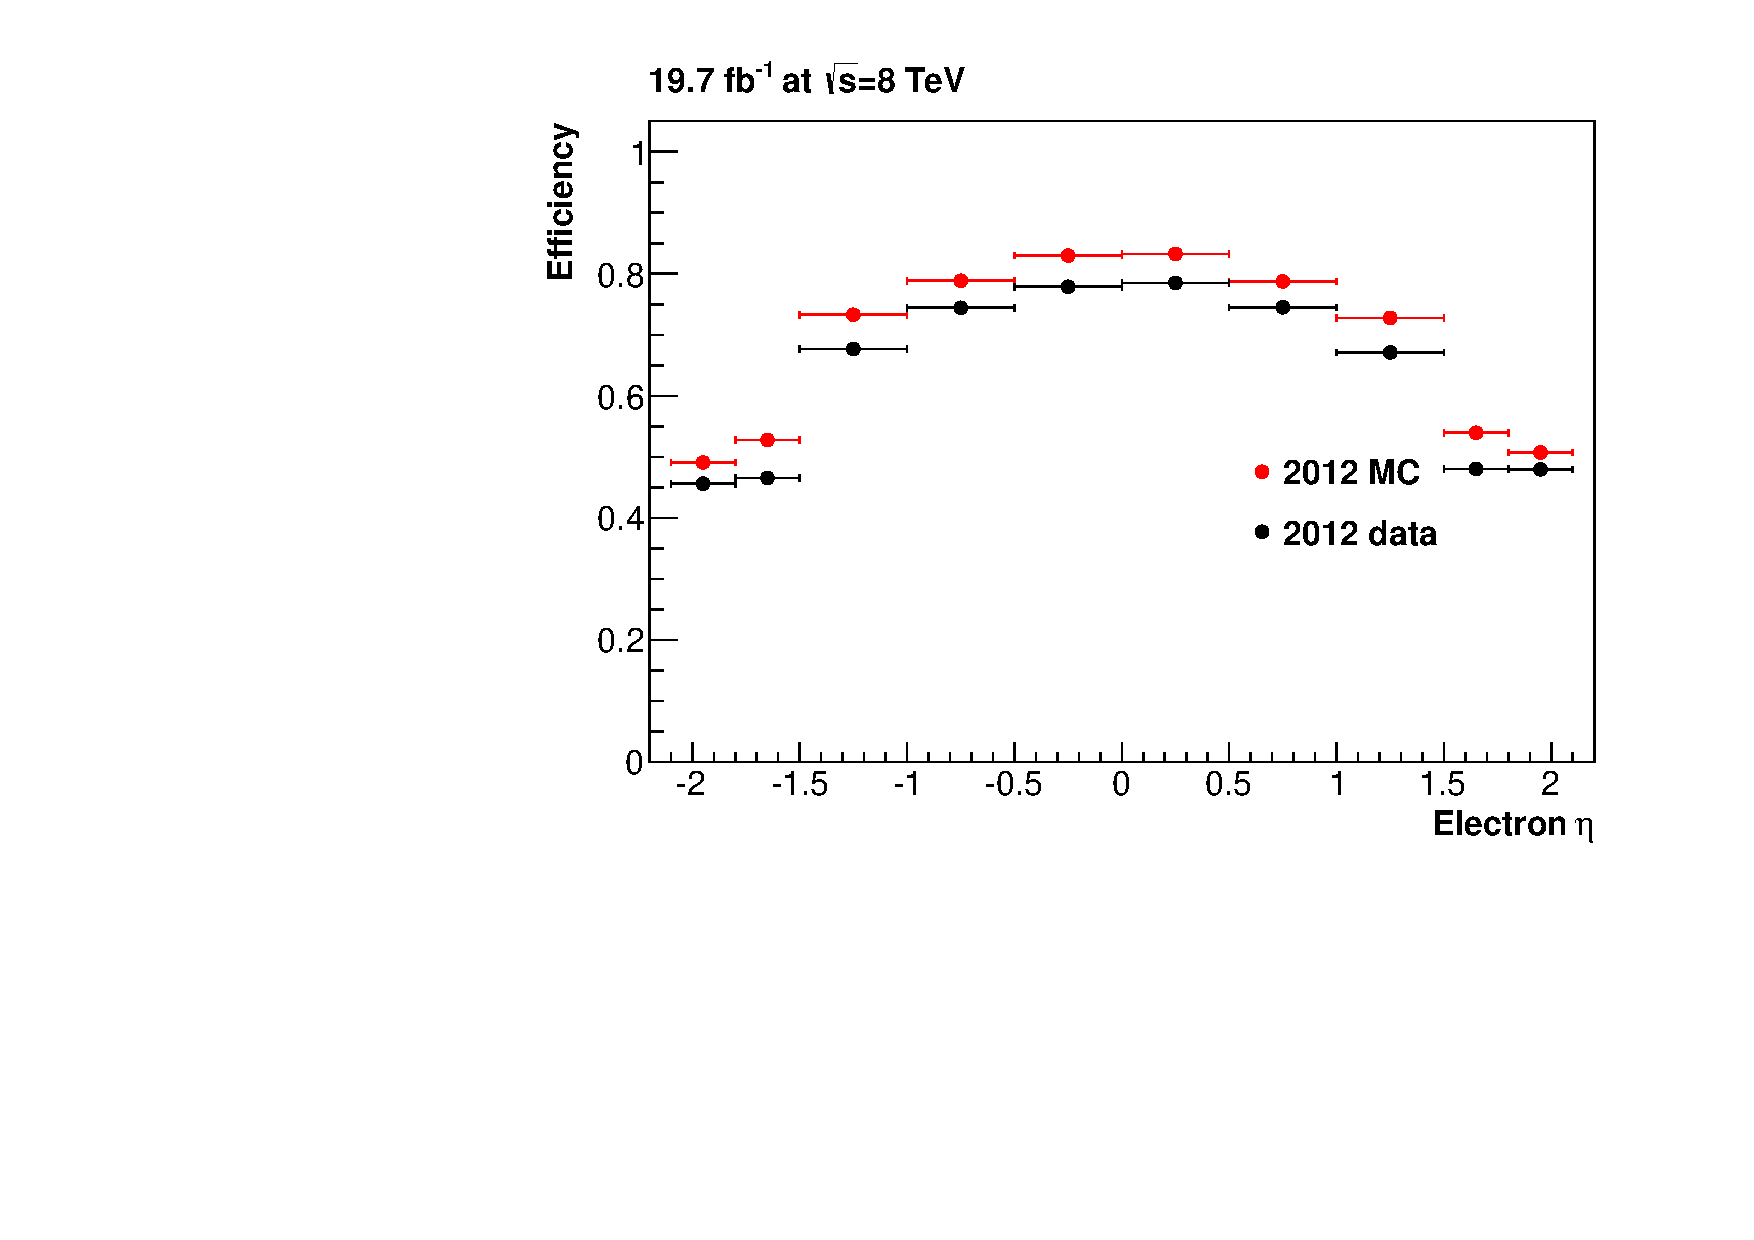
\includegraphics[width=0.5\textwidth]{plots/TagAndProbe/ElectronIdIsoEta2012DatavsMC.pdf}}
\subfloat[]{
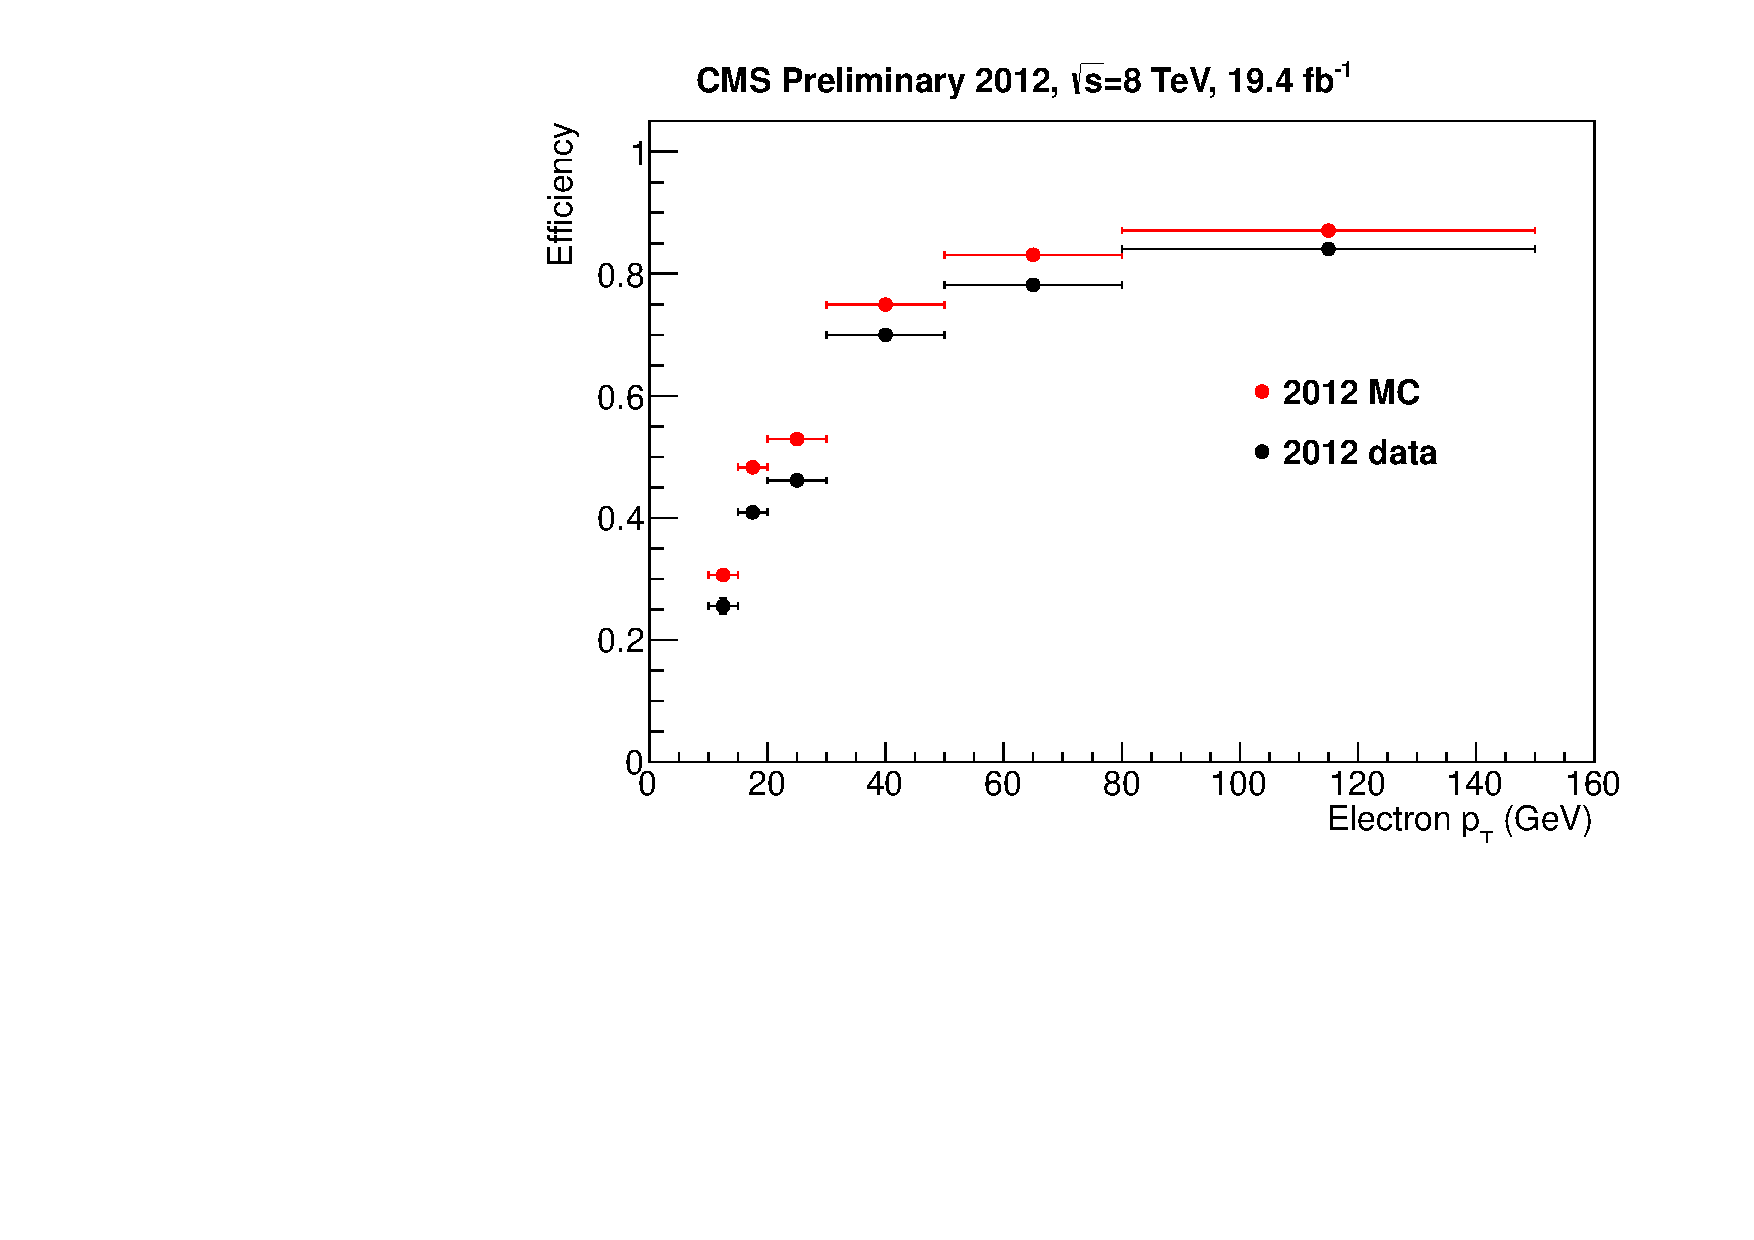
\includegraphics[width=0.5\textwidth]{plots/TagAndProbe/ElectronIdIsoPT2012DatavsMC.pdf}}
\caption{Combined electron ID and isolation efficiency in data and MC as a
function of (left) $\eta$ and (right) $\pt$}
\label{fig:electronIdIso}
\end{figure}

\begin{figure}[htb]
\subfloat[]{
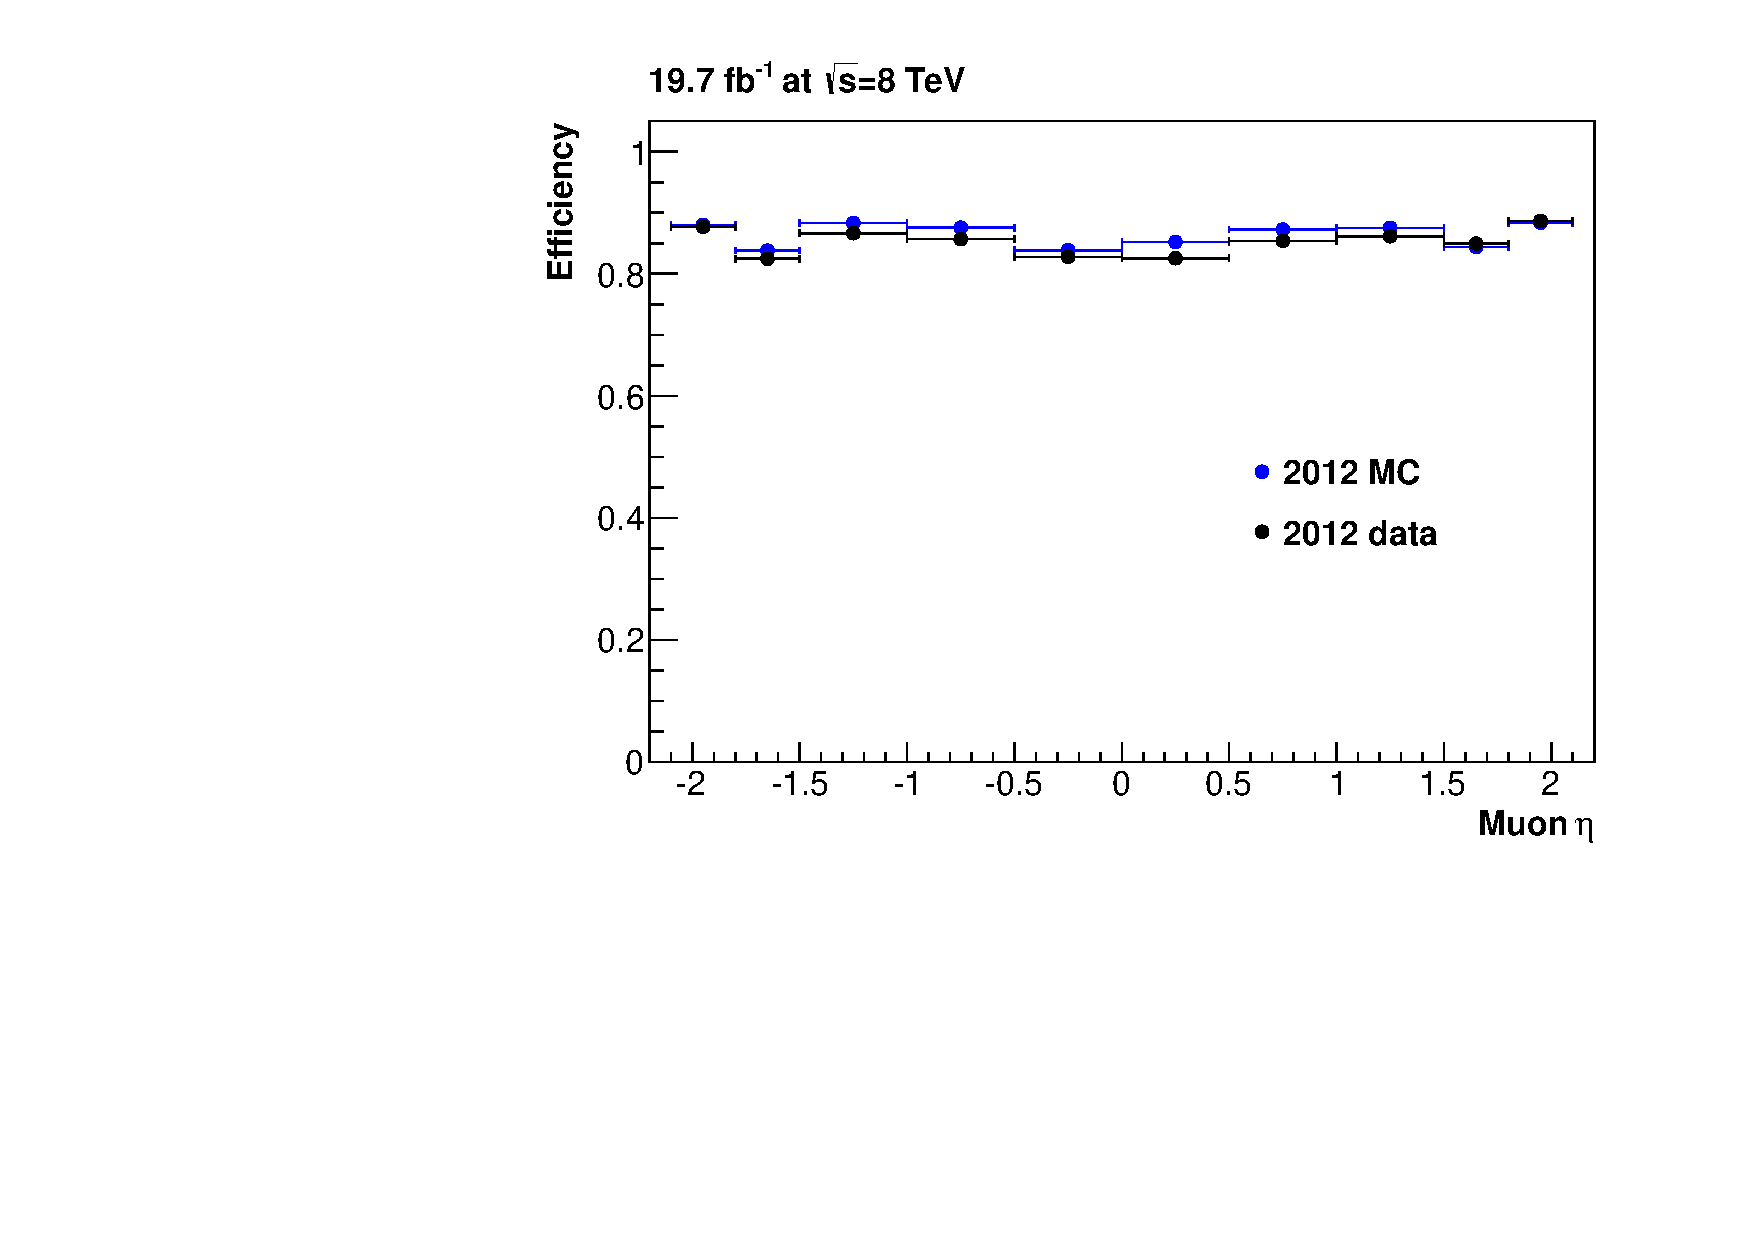
\includegraphics[width=0.5\textwidth]{plots/TagAndProbe/MuonIdIsoEta2012DatavsMC.pdf}}
\subfloat[]{
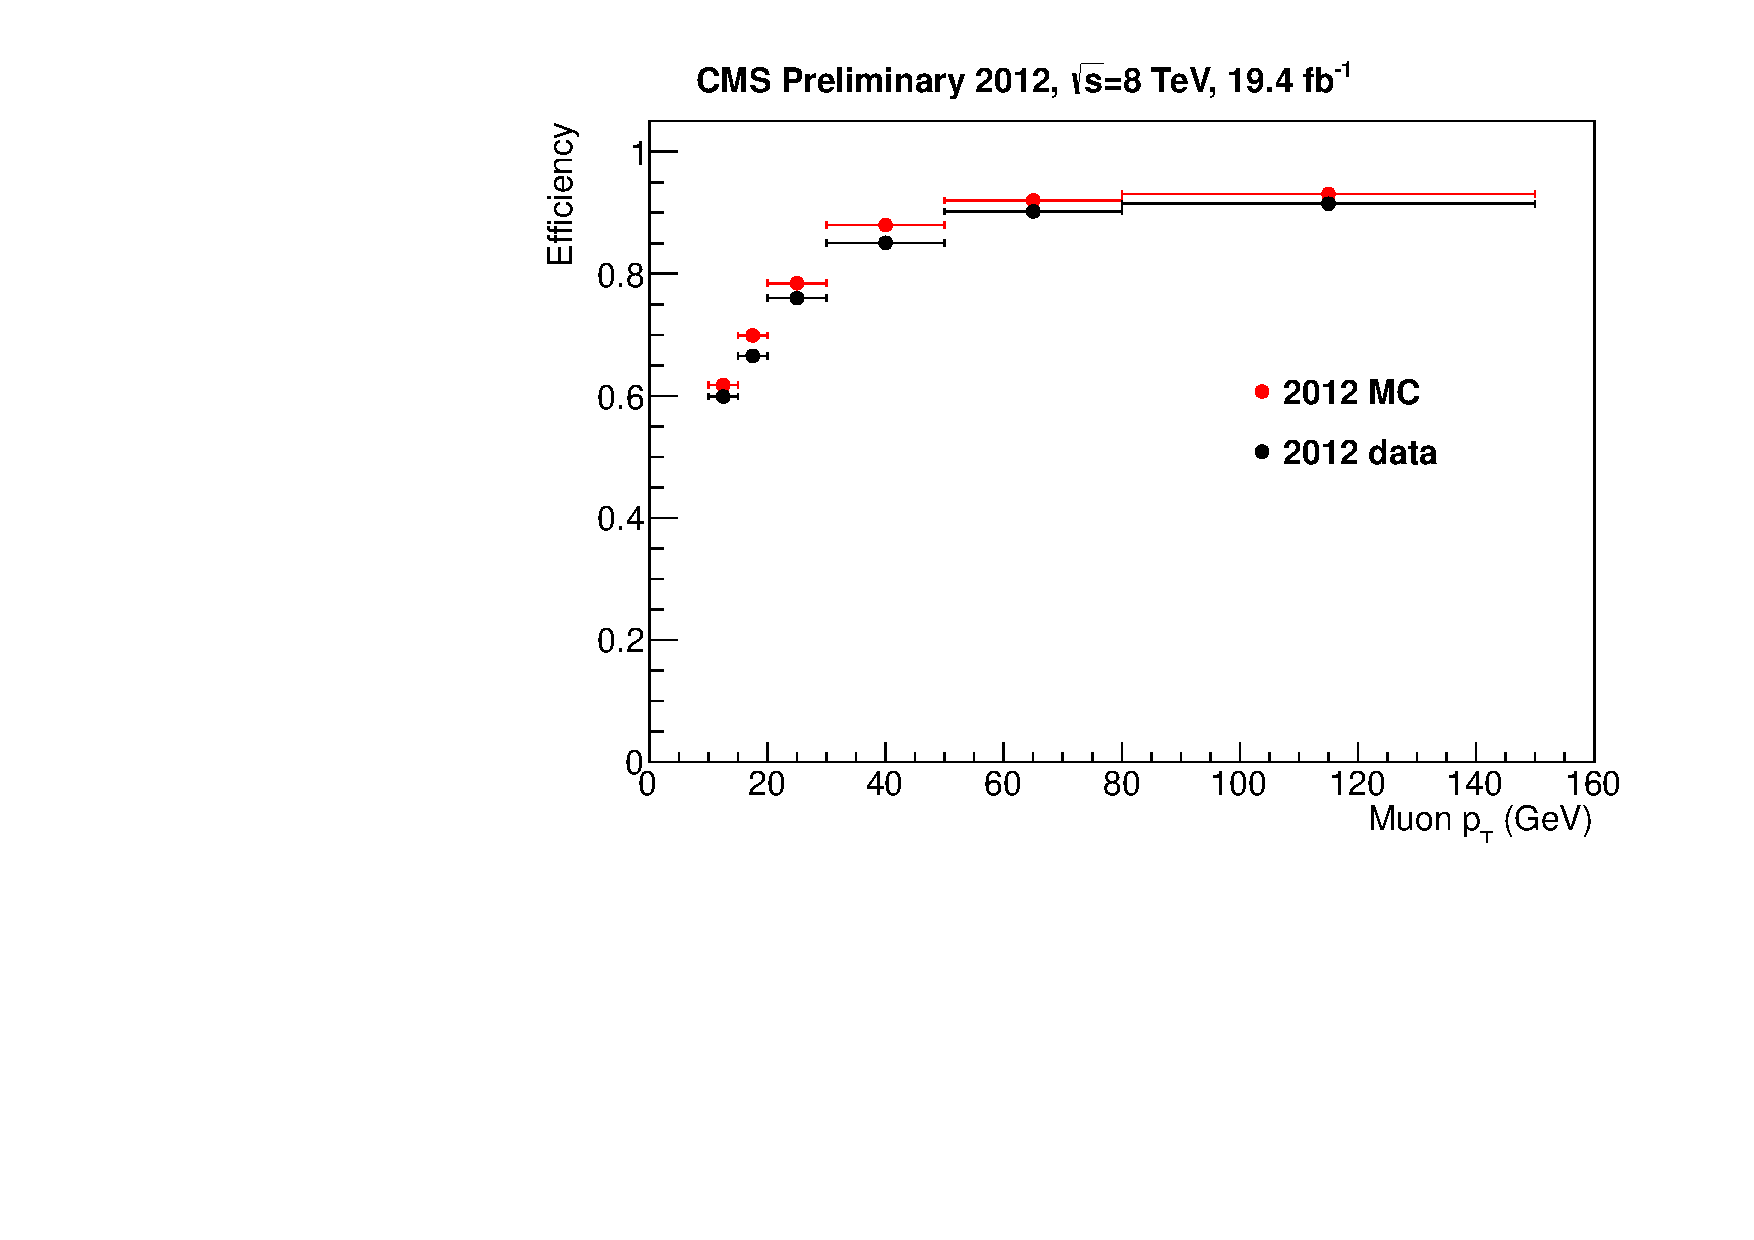
\includegraphics[width=0.5\textwidth]{plots/TagAndProbe/MuonIdIsoPT2012DatavsMC.pdf}}
\caption{Combined muon ID and isolation efficiency in data and MC as a function
of (left) $\eta$ and (right) $\pt$}
\label{fig:muonIdIso}
\end{figure}

The same method is used to measure the efficiencies of the trigger
in data and MC. In this case a probe is used which has already passed both ID
and isolation, and the passing probe condition is that the lepton is responsible
for firing the lepton leg of the lepton plus tau trigger. Figures
\ref{fig:electrontrg} and \ref{fig:muontrg} show the trigger efficiency as a
function of $\pt$ measured in both 2012 data and \ac{MC}. For the
electrons, the trigger is measured separately in the barrel and endcap
regions, which correspond to $|\eta| < 1.479$ and $|\eta| > 1.479$
respectively. For the muons, the trigger is measured in three regions, corresponding
to the different regions of the muon chambers as discussed in chapter
\ref{chap:detector}.

\begin{figure}[htb]
\subfloat[]{
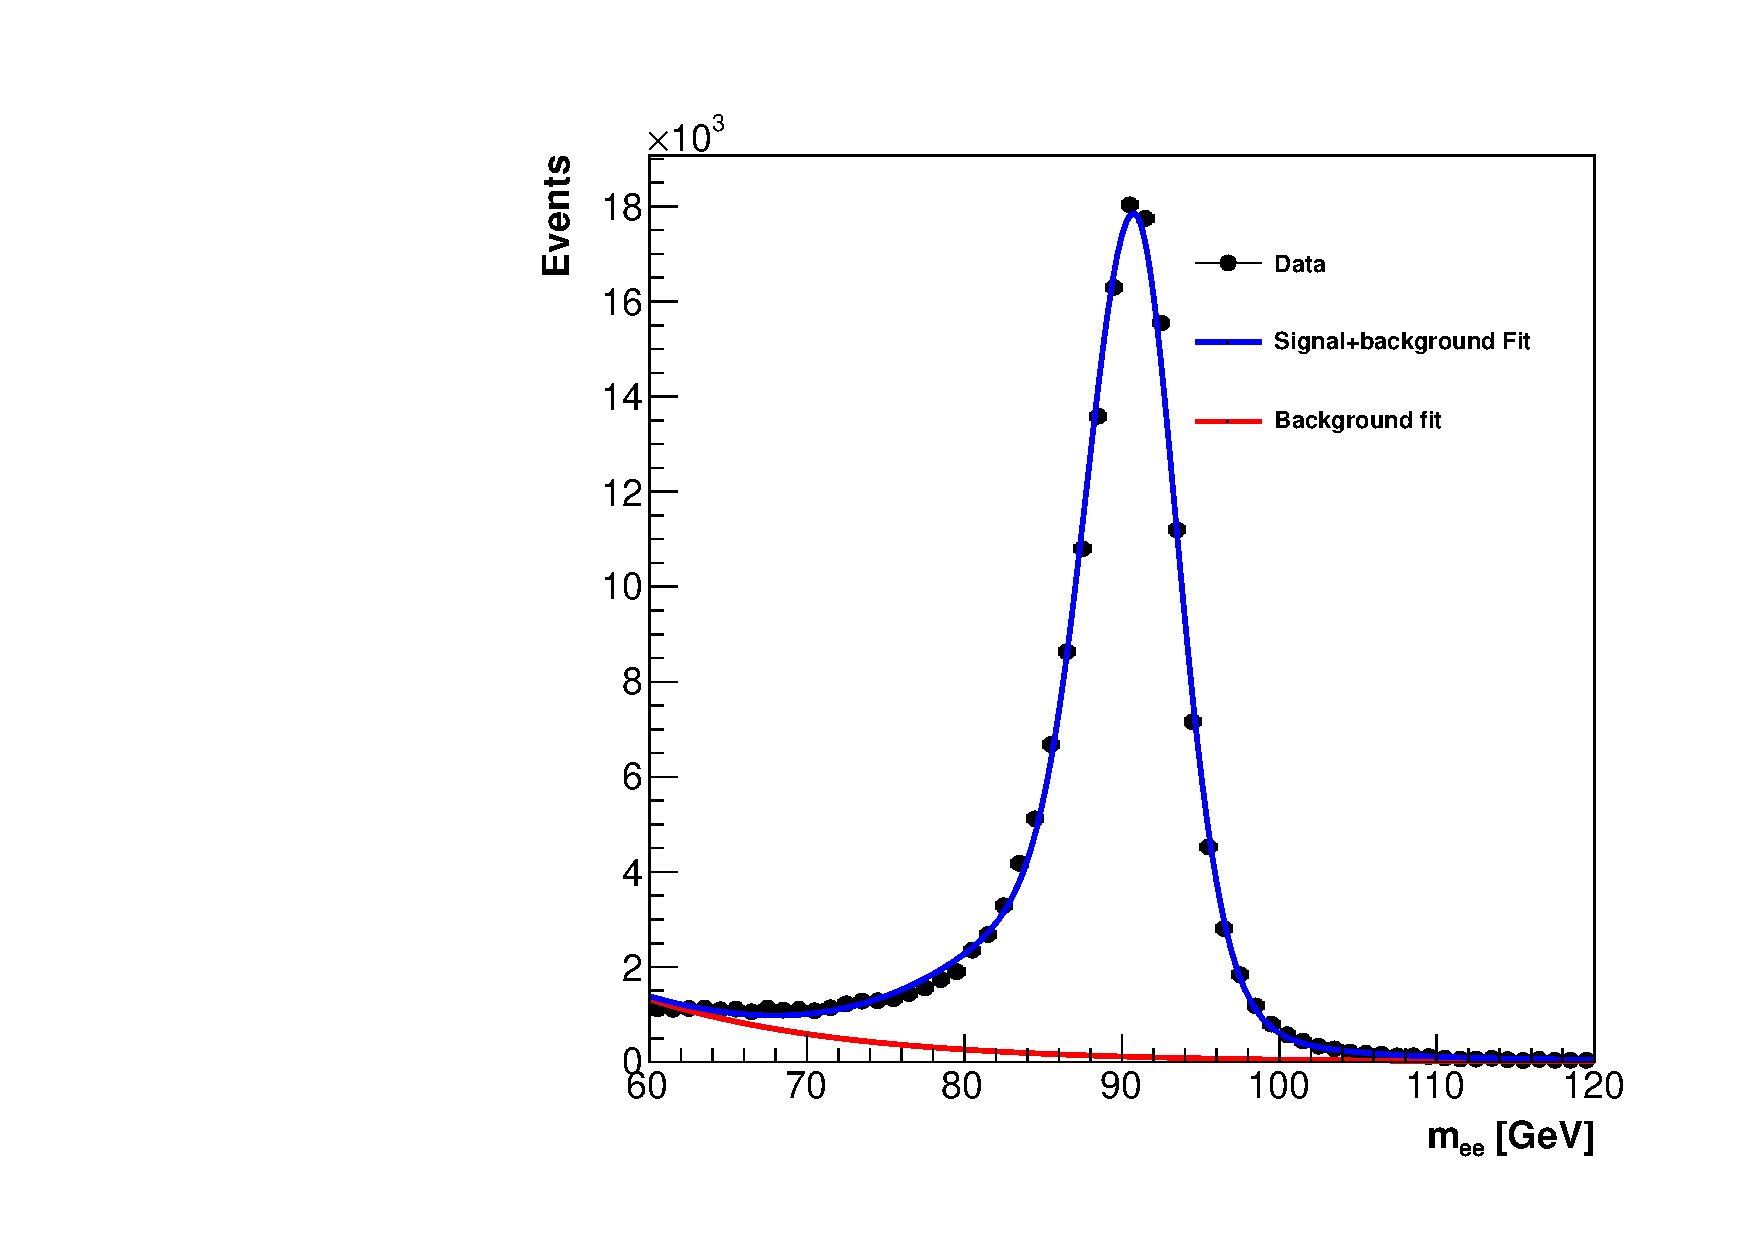
\includegraphics[width=0.5\textwidth]{plots/TagAndProbe/ee_TP_fit.pdf}}
\subfloat[]{
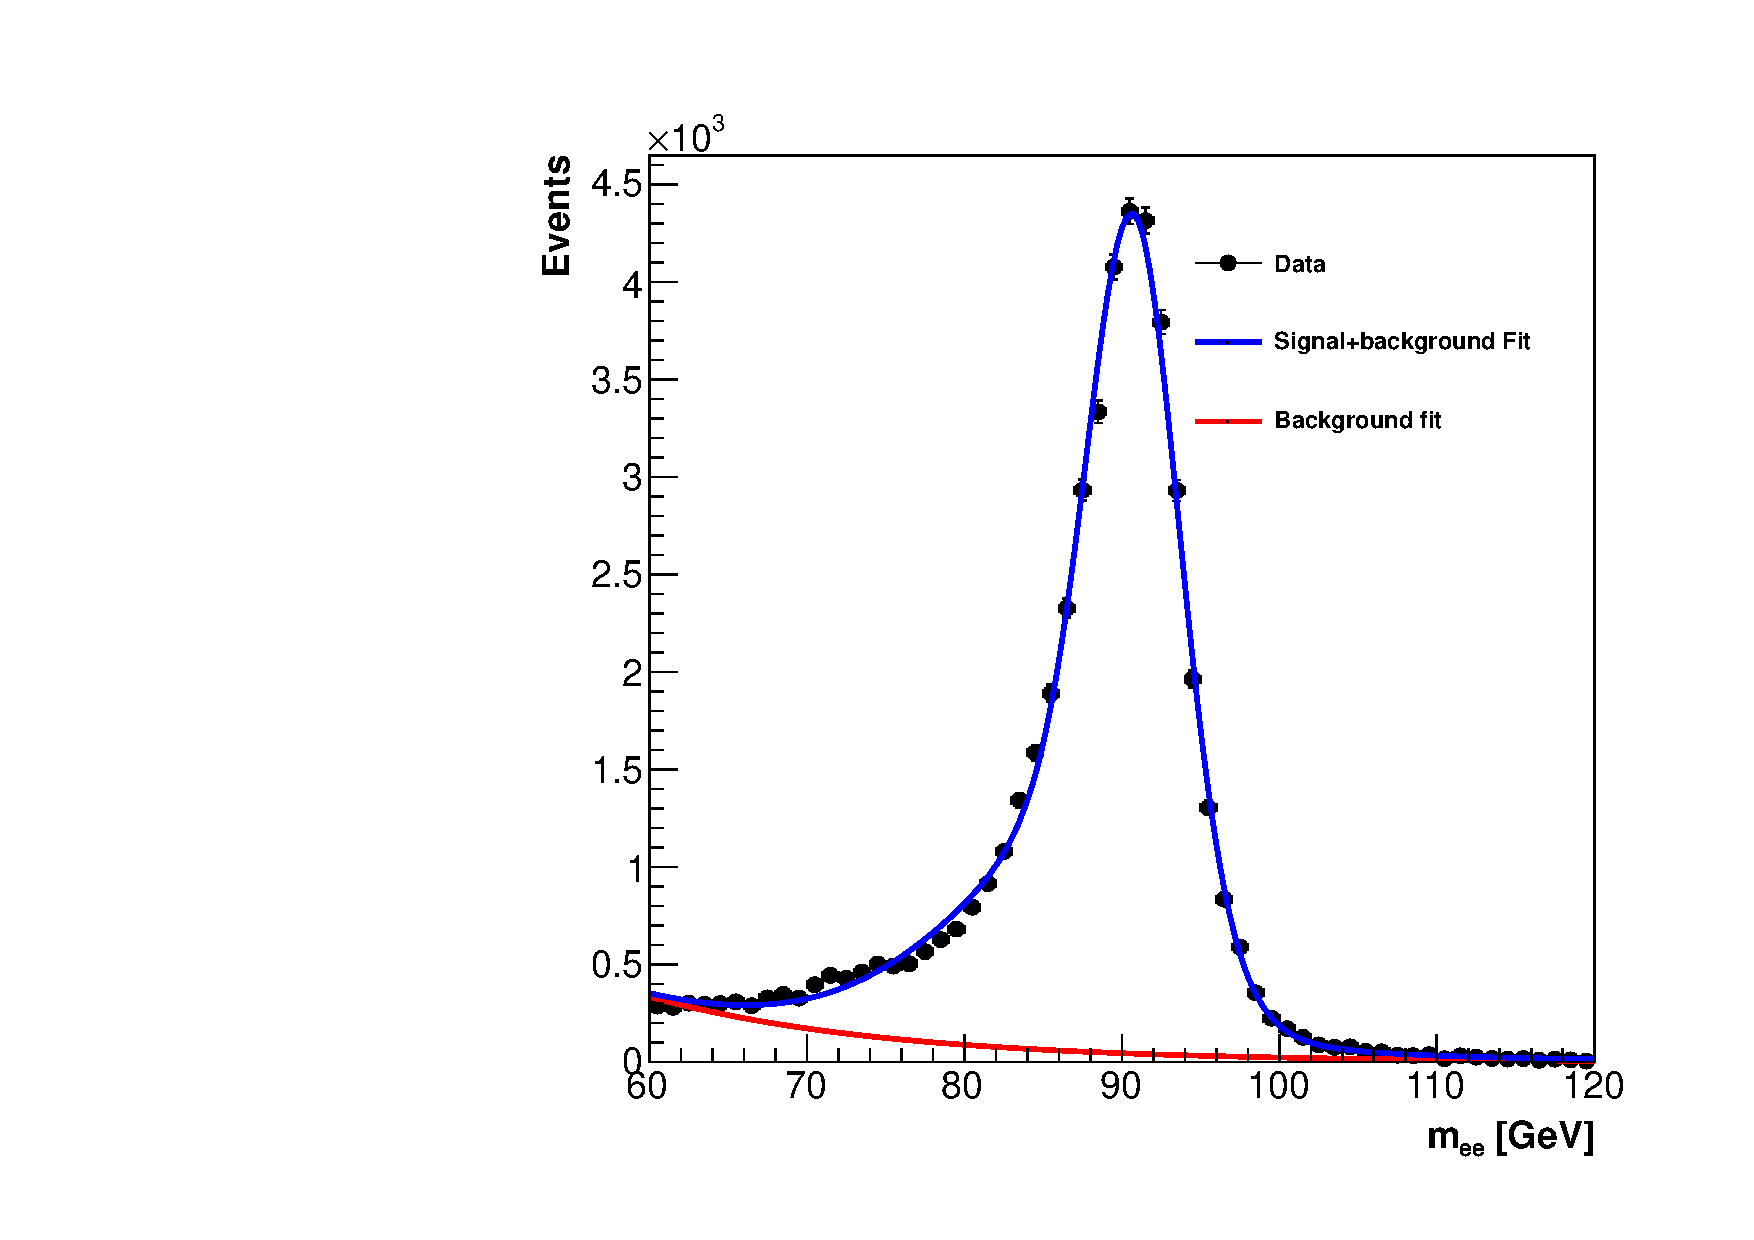
\includegraphics[width=0.5\textwidth]{plots/TagAndProbe/ee_TF_fit.pdf}}
\caption{Fitted $m_{ee}$ peaks for $\PZ\to\Pe\Pe$ tag and probe data events with a probe passing (a) and
failing (b) matching to the electron leg of the $\etau$ trigger. This example
fit is for electrons with $26 <\pt< 30~\GeV$ in the barrel. A separate function is fitted for the
background and signal ($\PZ\to\Pe\Pe$) contributions. The ratio of the integrals
of these two fits gives the trigger efficiency of the electrons, which is
approximately $80\%$ for this $\pt$ and $\eta$ range.}
\label{fig:tandp}
\end{figure}


\begin{figure}[htb]
\subfloat[]{
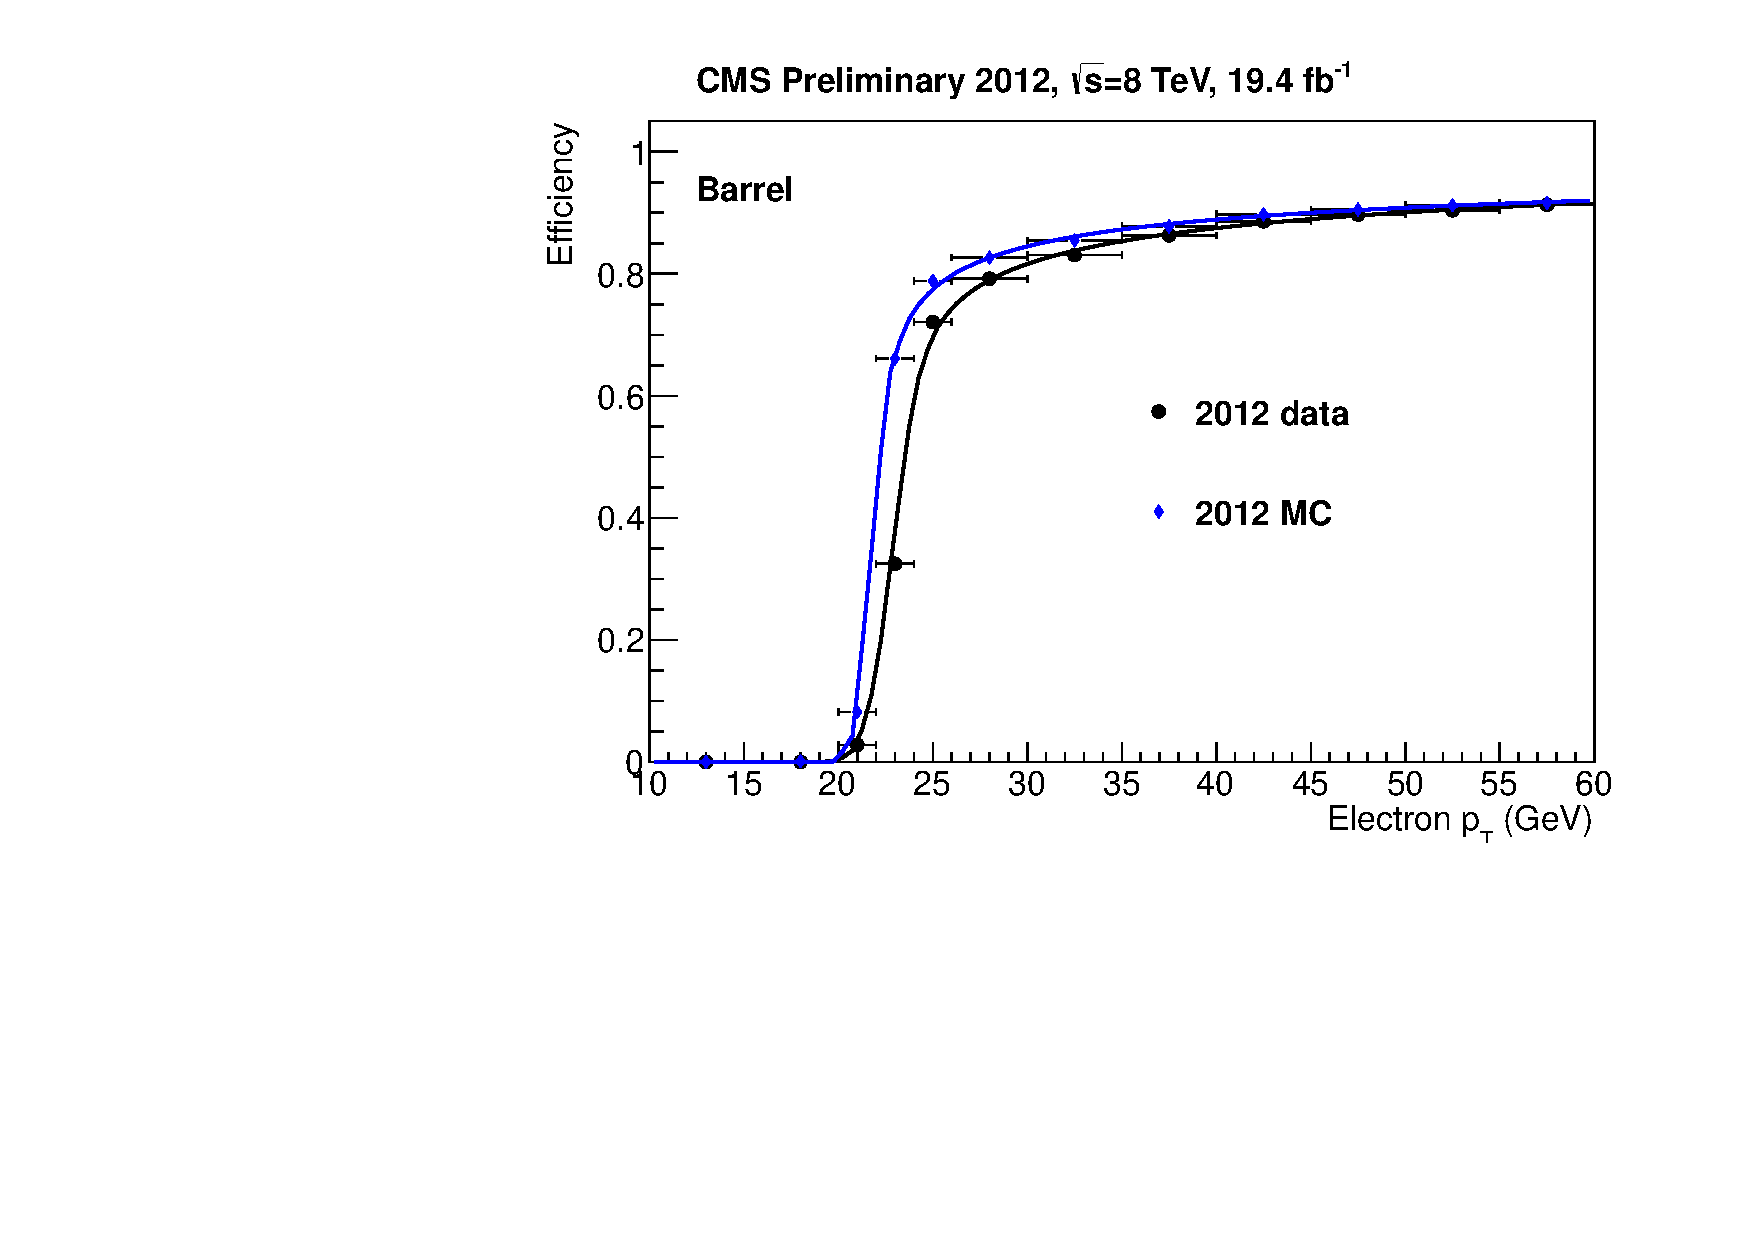
\includegraphics[width=0.5\textwidth]{plots/TagAndProbe/ElectronBarrel2012DatavsMC.pdf}}
\subfloat[]{
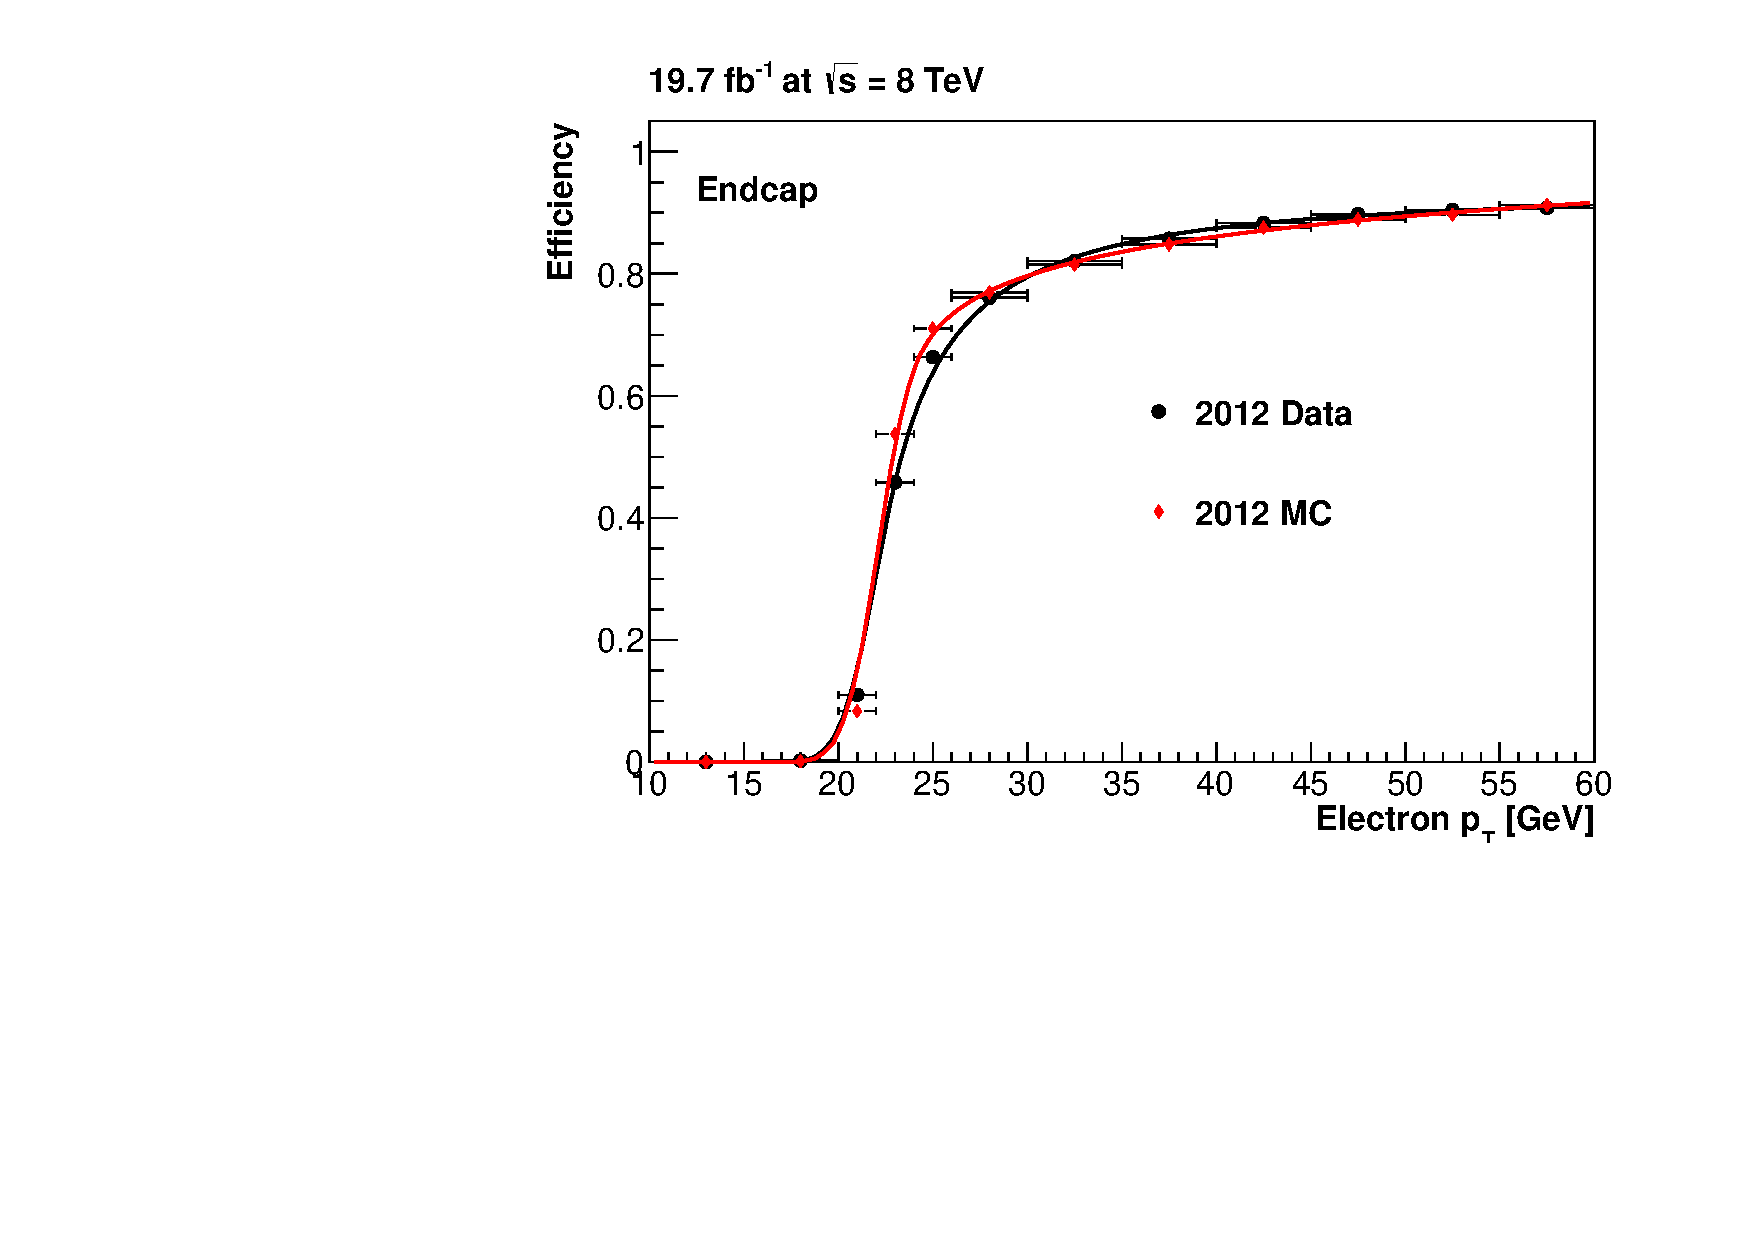
\includegraphics[width=0.5\textwidth]{plots/TagAndProbe/ElectronEndcap2012DatavsMC.pdf}}
\caption{Efficiency of the electron leg of the $\etau$ trigger as a function of electron $\pt$ measured
in 2012 data and MC in the (left) barrel and (right) endcaps.}
\label{fig:electrontrg}
\end{figure}

\begin{figure}[htb]
\subfloat[]{
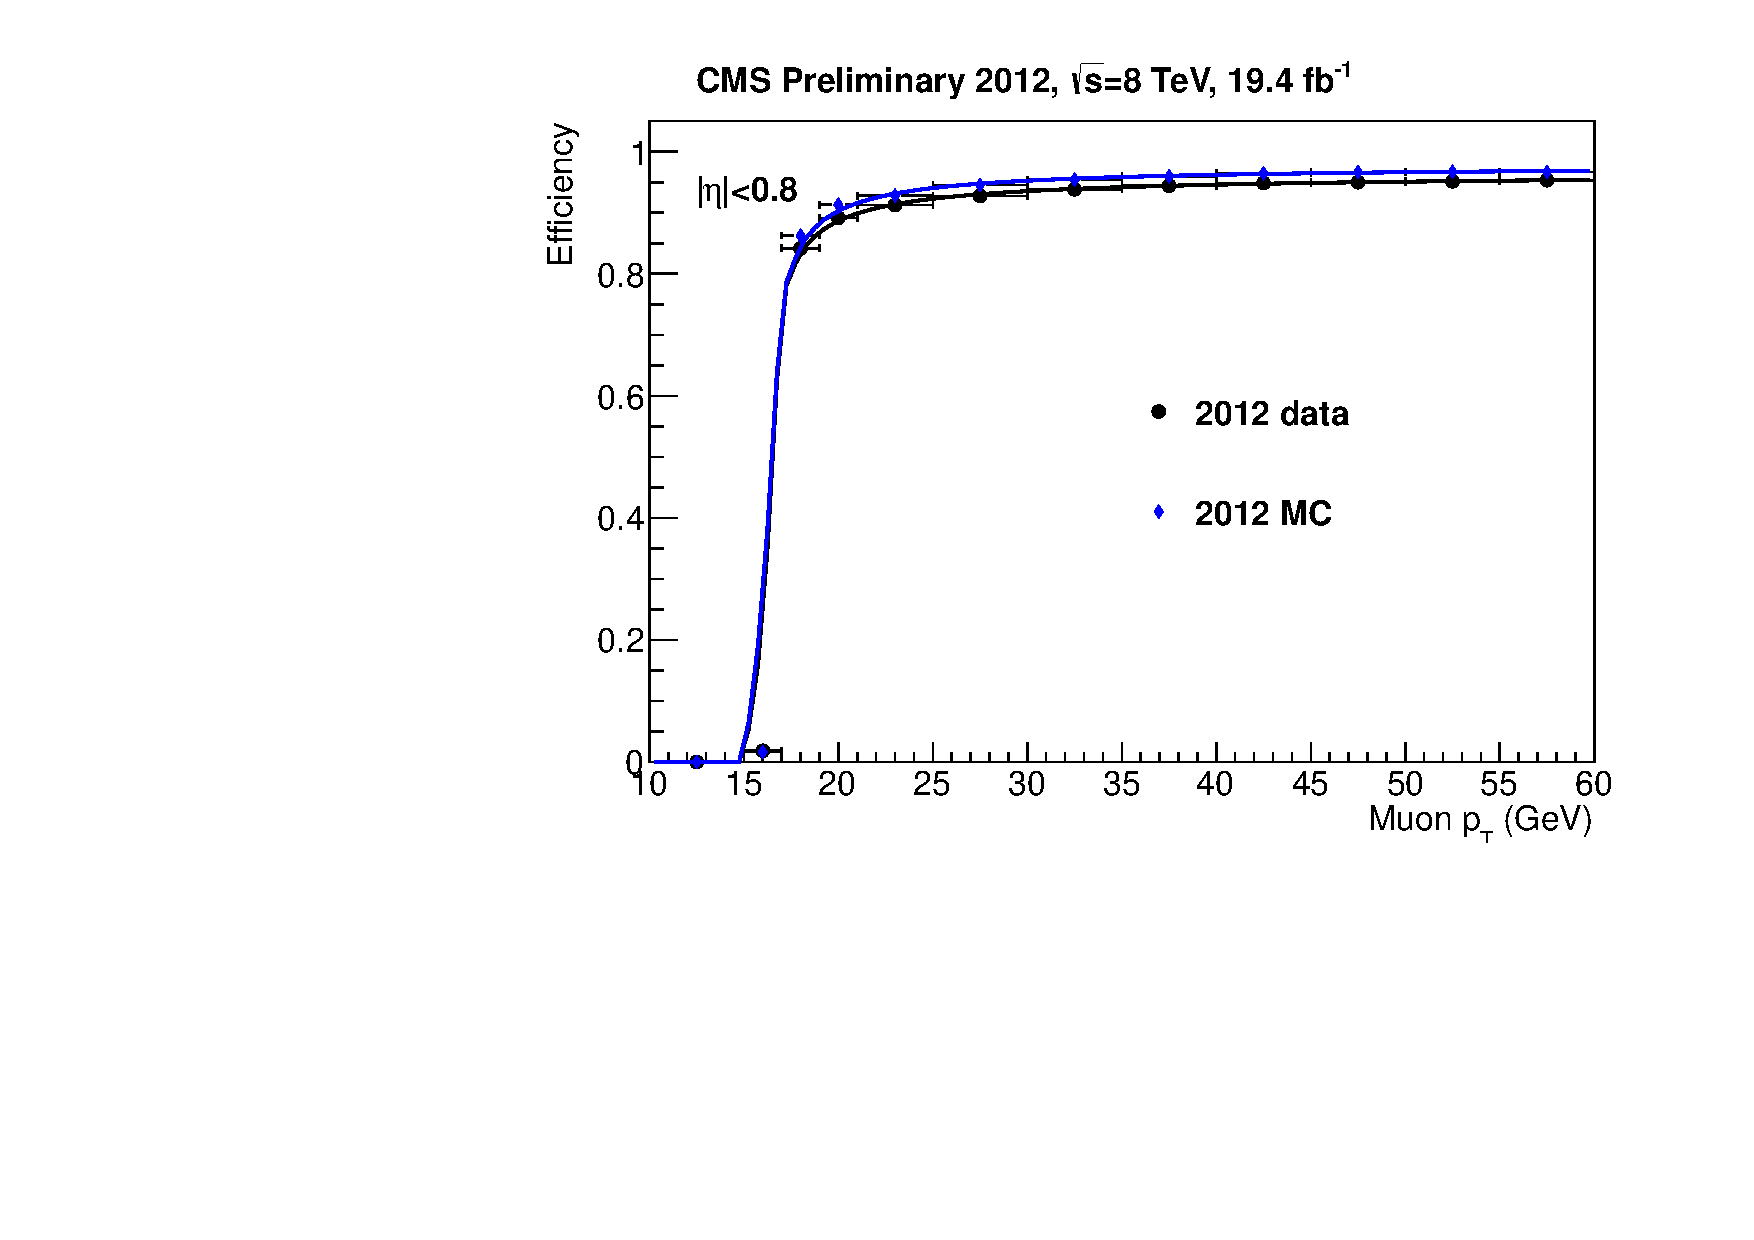
\includegraphics[width=0.5\textwidth]{plots/TagAndProbe/MuonAbsEta082012DatavsMC.pdf}}
\subfloat[]{
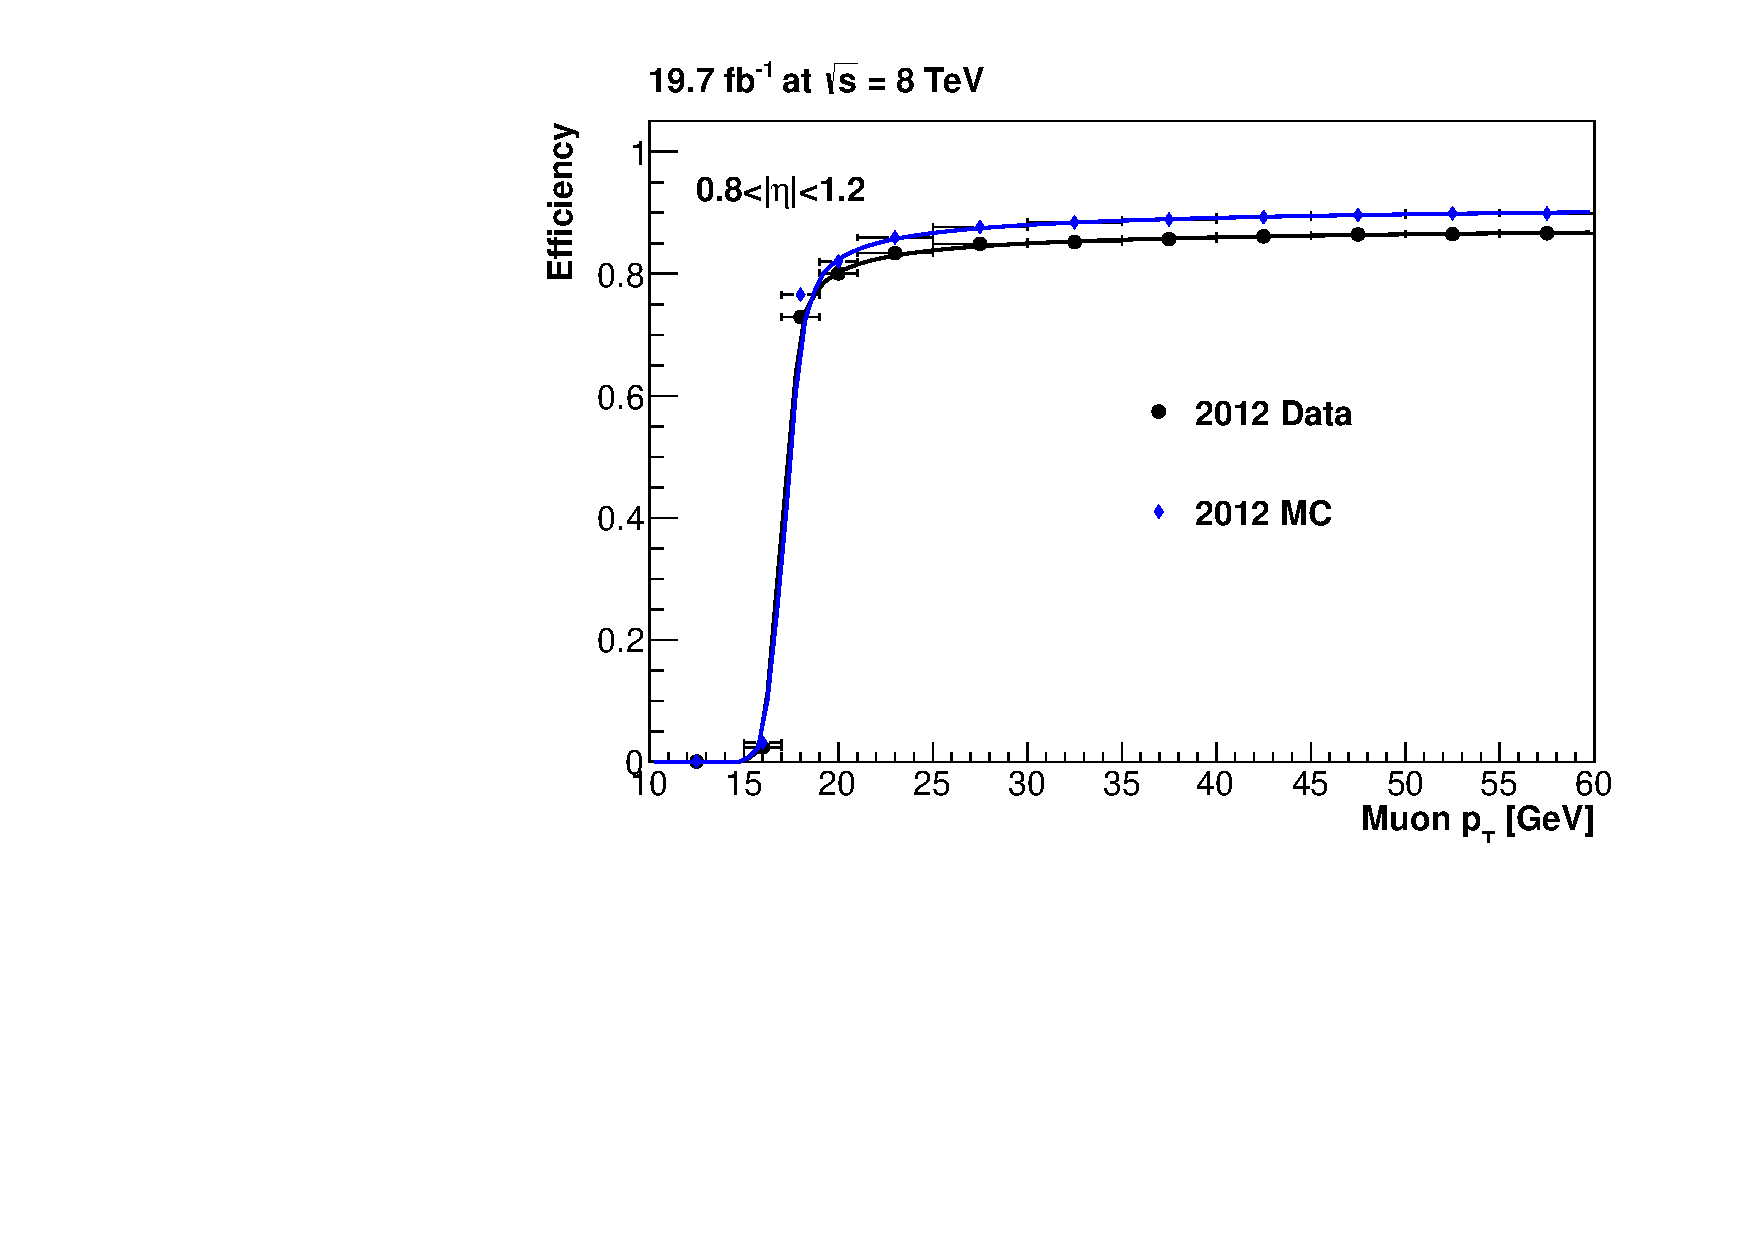
\includegraphics[width=0.5\textwidth]{plots/TagAndProbe/MuonAbsEta122012DatavsMC.pdf}}

\begin{center}
\subfloat[]{
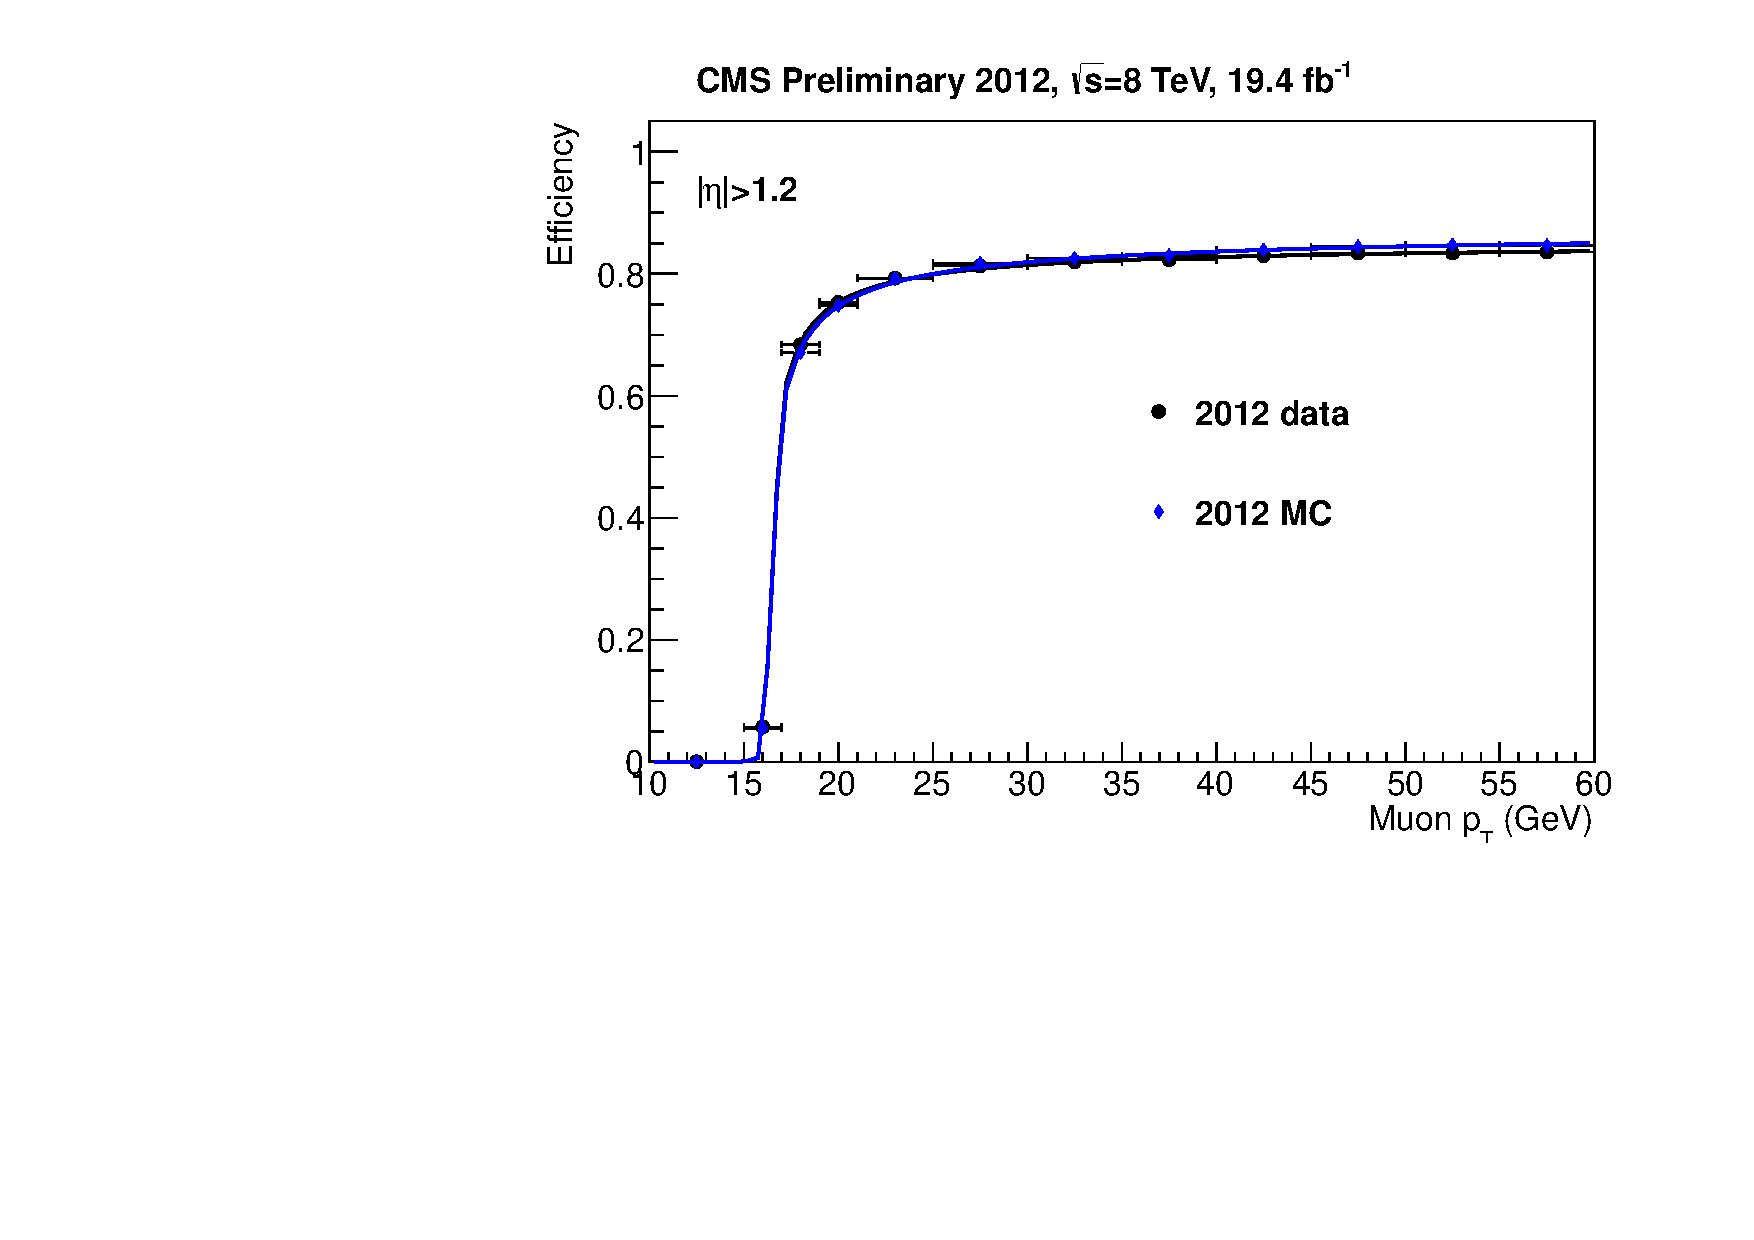
\includegraphics[width=0.5\textwidth]{plots/TagAndProbe/MuonAbsEndcap2012DatavsMC.pdf}}
\end{center}
\caption{Efficiency of the muon leg of the $\mutau$ trigger as a function of muon $\pt$ measured in
2012 data and MC in the region (top left) $|\eta|$ $<$ 0.8, (top right) 0.8
$<$ $|\eta|$ $<$ 1.2 and (bottom) $|\eta|$ $>$ 1.2.}
\label{fig:muontrg}
\end{figure}

\subsection{Other corrections}
\label{sec:othercorrections}

Several other data to \ac{MC} corrections are applied in this analysis, and are
discussed briefly here. More information on each correction can be found in
\cite{HIG-13-004}. 

Corrections for the tau trigger efficiency are 
obtained in a similar way as for the light leptons, using $\PZ\to\Pgt\Pgt\to\Pmu\Pgt_{h}$ events. As described in
section \ref{sec:taues}, a correction to \ac{MC} for the tau energy
scale is derived by fitting the di-tau mass and applied to the \ac{MC} samples
which contain real taus.

As mentioned in section \ref{sec:dataandMC}, a weight is applied to \ac{MC} such
that the pileup distribution matches that observed in data.

B-tagging is used in this analysis as a veto, to reduce the contribution of
$\ttbar$ background, and so the \ac{MC} must be corrected for differing b-tag
and light jet mis-tag efficiencies in data and \ac{MC}. The description of how
these efficiencies are obtained can be found in \cite{CMS-PAS-BTV-11-004} for
2011 data and \cite{CMS-PAS-BTV-13-001} for 2012 data. Since the categorisation 
depends only on the number of b-tagged jets (which should be 0 for selected events), 
we apply this efficiency using a promote/demote method to reclassify jets in \ac{MC} 
to make the overall b-tagging rate in the \ac{MC} match the data. This is done
by assigning each jet a probability defined as:
\begin{equation}
P(\text{demote})  = 1 - \text{b-tag}_{SF} \quad \text{for } \text{b-tag}_{SF} < 1 \\
P(\text{promote}) = \frac{\left(\text{b-tag}_{SF} -
1\right)}{\frac{\text{b-tag}_{SF}}{\epsilon_{MC}-1} } \quad \text{for } \text{b-tag}_{SF} > 1 ,
\end{equation}

where $\text{b-tag}_{SF}$ is the $\pt$ and $\eta$ dependent scale factor and
$\epsilon_{MC}$ is the tagging efficiency in \ac{MC}.

A correction is applied in the \ac{SM} gluon-gluon fusion signal
samples to account for the difference in Higgs $\pt$ distribution at \ac{NNLO}
compared with \ac{NLO}. Events are reweighted to make the Higgs $\pt$
distribution match that obtained in the \ac{NNLO} \textsc{HRes}~\cite{deFlorian:2012mx} program. 
A correction for the difference between the finite and infinite top
mass approximations is also applied \cite{Grazzini:2013mca}.

%A $\pt$-dependent re-weighting is applied to $t \bar{t}$ events to better match
%the top quark $\pt$ distribution observed in data. 

The contribution of $Z/\gamma^{*} \to ee$ background to the $\etau$ channel
is additionally corrected by $e \to \tau_{had}$ fake-rate \ac{MC} to data
scale factors. These are obtained by fitting the distribution of the $\Pe$ +
$\Pgt_{h}$ visible mass for taus reconstructed in different decay modes. 

\section{Systematic Uncertainties}
\label{sec:systematics}

The systematic uncertainties consist of two different types:

\begin{itemize} 
\item Normalisation uncertainties: these affect the yield of a particular background or
signal.
\item Shape uncertainties: these affect the shape of the signal or background,
i.e. the number of signal or background events in a particular bin rather
than the overall number.
\end{itemize}

The way in which these different types of uncertainties are incorporated in the
final results is described in section \ref{sec:signalextraction}. The different
sources of uncertainties and their chosen values is described separately for the 
normalisation and shape uncertainties.

\subsection{Normalisation Uncertainties}
\label{sec:systematicUncertainties_yield}

\subsubsection{\textbf{ID, isolation and trigger efficiencies for the electrons, muons and
hadronic taus}}
As discussed in the previous section, data to \ac{MC} scale factors are measured for this 
analysis and applied to correct \ac{MC}. The estimated uncertainty in these
measurements are combined in quadrature. For the electrons and muons, this
amounts to a $2\%$ normalisation uncertainty, which is applied to all
backgrounds in which the yield is taken from MC and signal.
For the hadronic taus a $6\%$ uncertainty
is measured on the tau identification efficiency using 
$Z/\gamma^{*} \to \Pgt\Pgt \to \Pmu\Pgt_{h}$ events~\cite{Chatrchyan:2012zz}. 
For the hadronic tau leg of the trigger, the uncertainty is $3\%$ for the $\etau$ and $\mutau$ triggers.
These uncertainties are applied to signal and all backgrounds in which the yield
is taken from \ac{MC}.

\subsubsection{\textbf{b-tag scale factors}} 
Uncertainties on b-tagging efficiencies and mistag rates as function of jet
$\pt$ and $\eta$ are incorporated through variations of the scale factors
described in the previous section within their estimated uncertainties to modify
the promote/demote probabilities. This results in an overall change in yield for
backgrounds and signal as a result of the b-jet veto. For those backgrounds
with a non-negligible variation as a result of this uncertainty the yield change
is applied as a normalisation uncertainty. The largest effect of this
uncertainty is on the $\ttbar$ background which contains real b-jets and can
vary by up to $10\%$ as a result of this uncertainty. The values of the uncertainties 
are determined as part of the measurement of the efficiencies as described in 
\cite{CMS-PAS-BTV-11-004} for 2011 data and \cite{CMS-PAS-BTV-13-001} for 2012 data.

\subsubsection{\textbf{$\MET$ scale uncertainty}}
Uncertainties on \MET resolution and response are accounted for
by varying the $Z$-recoil correction parameters within the uncertainties
determined within the recoil correction method.
This can result in a change in yield as a result of the $m_{\text{T}}$ cut, and
also affects the $m_{\Pgt\Pgt}$ distribution. In the $\etau$ channel it also directly
effects the 1--jet categories via the $\MET > 30~\GeV$ cut. The $\MET$ scale
uncertainty is controlled to within $5\%$ \cite{CMS-PAS-JME-12-002} by the recoil fits and the resulting
uncertainty on each category is similar. 

\subsubsection{\textbf{Jet energy scale}}
Uncertainty on jet energy scale was discussed in section
\ref{sec:JEC}. This uncertainty can change the number of events in
each category via the change in jet $\pt$ and $m_{jj}$. Thus the largest
variations as a result of this uncertainty can be found in the VBF categories
and are in the range of $5$-$15\%$. 

\subsubsection{\textbf{Background Normalisation}}
The systematic uncertainty of the $\ZToTauTau$ estimate is significantly reduced
through the use of embedded samples. However, systematics must be evaluated for
the embedding process to account for imperfections in the removal of the
$\PZ\to\Pgm\Pgm$ event. This process is studied by applying the embedding
procedure to $\PZ\to\Pmu\Pmu$ \ac{MC} and comparing with pure $\ZToTauTau$
\ac{MC}, and an uncertainty of approximately $5\%$ in the category efficiencies
is observed. An overall uncertainty of $3\%$ on the inclusive normalisation from
$\PZ\to LL$ \ac{MC} is also applied, to both the $\ZToTauTau$ and
$\PZ\to\ell\ell$ predictions.

The normalization of the $\WJets$ background is obtained from data, 
using the high $m_{\text{T}}$ sideband extrapolation method described in
section~\ref{sec:backgroundEstimation_WplusJets}. Uncertainties on the
extrapolation factor obtained using \ac{MC} are found to be in the region of
$10$-$25\%$ depending on category. These are estimated by comparing the shape of
the $m_{\text{T}}$ distribution in data and \ac{MC} in a sample of
$\PZ\to\Pgm\Pgm$ events in which one muon is treated as invisible in the event
reconstruction to mimic a $\PW$ decay. 

The uncertainty on the normalization of QCD background is obtained by adding the
statistical uncertainty on the yield of events selected in the QCD dominated control regions
described in section~\ref{sec:backgroundEstimation_QCD} in quadrature with the
uncertainty on opposite sign - same sign factor of 1.06, which is found to be
10$\%$ as measured in an anti-isolated sample.

The uncertainty on the $t \bar{t}$ cross-section amounts to $10\%$, and on the single top and di-boson
production cross-sections amounts to $15\%$ \cite{Chatrchyan:2013oev,Chatrchyan:2012ep}.
 
\subsubsection{\textbf{$\Pgt_{h}$ fake-rates}} 
The uncertainty on the $\Pe \to \Pgt_{h}$ fakerate is determined as part of
its measurement. This amounts to an uncertainty of $30\%$, correlated between
$\Pgt_{h}$ candidates reconstructed in any tau decay mode. 
The uncertainty on the rate of $\Pmu \to \Pgt_{h}$ fakes amounts to $30\%$.
The uncertainty on the rate of jets faking taus is $20\%$ and primarily affects
the $\PZ\to\ell\ell$ background, and not the QCD or \WJets which are normalised
using data driven methods.

\subsubsection{\textbf{Luminosity}} 
The uncertainty on the luminosity amounts to $2.2\%$ for the 2011 data and
$2.6\%$ for the 2012 data as described in \cite{CMS-PAS-SMP-12-008,CMS-PAS-LUM-13-001}.
This uncertainty is applied to the signal and to $Z/\gamma^{*} \to \ell\ell$, $Z/\gamma^{*} \to
\tau\tau$, $t \bar{t}$, single top and di--boson backgrounds. 
The normalization of the $W$ + jets and QCD backgrounds is obtained from data and hence not subject to the luminosity uncertainty.

\subsubsection{\textbf{Theoretical Uncertainties}} 
Theoretical uncertainties on the \ac{MC} predictions of the different signal
contributions are estimated in the form of an uncertainty on the acceptance in
each category. The \ac{PDF} uncertainty is estimated by calculating the
acceptance with several different \ac{PDF} sets and taking the largest possible
variation. The uncertainties as a result of the choice of \ac{PDF} amount to
approximately $2\%$ for gluon fusion and $1\%$ for \ac{VBF}. The uncertainties
on the inclusive cross-sections for gluon-fusion and \ac{VBF} are $7.5\%$ and
$2.8\%$ respectively from
\cite{LHCHiggsCrossSectionWorkingGroup:2011ti,Dittmaier:2012vm,Heinemeyer:2013tqa}.

Uncertainties due to the renormalisation and factorisation scale uncertainties
are around $5$-$20\%$ for gluon fusion and $1$-$5\%$ for \ac{VBF} dependent on
category. An additional uncertainty on the gluon-fusion contribution in the
VBF categories is estimated to account for the fact that the gluon-fusion is
simulated using \textsc{powheg} which only includes up to one jet in the matrix
element calculation. This is done by comparing the acceptances from other
generators, \textsc{madgraph}, \textsc{powheg+minlo} \cite{Hamilton:2012np} and
\textsc{mc@nlo} \cite{Frixione:2002ik}, resulting in an uncertainty of $30\%$.
Uncertainty in the underlying event simulation and parton showering is between
$2$ and $10\%$ depending on the category. 


\subsection{Shape Uncertainties}
\label{sec:systematicUncertainties_yield}

\subsubsection{$\tau_{had}$ energy scale} 
When studying mass distributions, the shape of the distribution is directly
dependent on the energy scale of the objects used in calculating the mass. Thus the
$m_{\Pgt\Pgt}$ shape is sensitive to the tau energy scale.
To incorporate this uncertainty, the energy scale of hadronically decaying taus is varied by $3\%$,
which is constrained by fits to the tau mass discussed in section \ref{sec:taues}.

\subsubsection{\textbf{$Z \to \ell\ell$ lepton energy scale}}
A shape uncertainty is also added for the $Z \to \ell\ell$ contribution for the
events where a lepton fakes a hadronic tau, to account for the effect of the energy 
scale of the lepton fake. This energy scale mismeasurement is estimated to give a 
shift of up to $2\%$ in the mass shape of the contribution, and hence a shape systematic amounting to the
$2\%$ shift up and down is included to cover for this effect.

\subsubsection{\textbf{Bin-by-bin statistical uncertainties}}
As described when discussing the background methods, selections are often
relaxed to obtain smooth templates for certain backgrounds in the most signal
sensitive categories. Despite this, low statistics in background templates must
still be accounted for in the fit. This often affects particular bins in the
template more than others, in particular at low or high $m_{\Pgt\Pgt}$ values
where event statistics are naturally lower. For these bins the statistical
uncertainty in the bin is considered a single uncorrelated source of
uncertainty, using a method described in \cite{Barlow1993219}. 

\section{Results}
\label{sec:results}

\subsection{Signal Extraction}
\label{sec:signalextraction}

The discriminating distribution used for signal extraction is the di-tau mass,
reconstructed using the SVFit algorithm described in section \ref{sec:svfit}. 
The methods employed in the statistical
interpretation of the data were developed by the LHC Higgs Combination Group and
are common methods used across the ATLAS and CMS experiments \cite{LHC-HCG-Report}.

The final $m_{\Pgt\Pgt}$ distribution for each category of each channel gives
us a prediction for the number of expected background events and the predicted number of signal
events in the presence of a \ac{SM} Higgs. From the observed data, we can assess
the consistency of this data with either the background only or
signal-plus-background hypotheses. We use all bins of the $m_{\Pgt\Pgt}$
distribution for this, i.e. we perform a shape analysis rather than just a
counting experiment. Thus we build a likelihood for an observed dataset,
dependent on the predictions for signal and background and taking into account
the systematic uncertainties described in the previous section.

The likelihood function $\mathcal{L}$ is given by the product of Poisson probabilities 
$Poisson(n_{i} \vert \nu_{i}(\mu, \theta))$ to observe $n_{i}$ events in each bin
$i$ of the $m_{\Pgt\Pgt}$ distribution:
\begin{equation}
\mathcal{L} = \prod_{i} \mathrm{Poisson}(n_{i} \vert \nu_{i}(\mu, \theta)) \cdot
\prod_{j} \mathrm{Constraint}(\theta_{j}, \tilde{\theta}_{j}),
\label{eq:LikelihoodFunction}
\end{equation}
with
\begin{equation}
\mathrm{Poisson} ( n_{i} \vert \nu_{i}(\mu, \theta )) = \frac{\nu_{i}^{n_{i}}}{n_{i}!} \exp ( -\nu_{i} ),
\label{eq:PoissonDistribution}
\end{equation}
where we denote by $\nu_{i}$ the number of events expected in that bin,
given by the sum of expected signal plus expected background events,
which are given by $\mu \cdot s_{i}$ and $b_{i}$ respectively.
The parameter $\mu$ is known as \emph{signal strength modifier}. 
It represents the unknown rate of the signal and can be given in reference to a
benchmark cross-section times branching ratio, in this case that of the \ac{SM}
Higgs. Background-only hypothesis implies $\mu = 0$ and any signal hypothesis $
\mu > 0$, with \ac{SM} Higgs predictions corresponding to $\mu = 1$.
Both the number of signal and the number of background events expected in bin $i$ 
are functions of a set of nuisance parameters $\theta$:
$s_{i} = s_{i} ( \theta )$ and $b_{i} = b_{i} ( \theta )$.
Individual components $\theta_{j}$ each represent one of the systematic uncertainties
discussed in section~\ref{sec:systematics}.

The first product in Eq.~\ref{eq:LikelihoodFunction} extends over all bins $i$
of the $m_{\tau\tau}$ distributions in all of the 0--jet, 1--jet and VBF categories 
for the $\etau$ and $\mutau$ channels, as well as the other channels included in
the final combination: $\emu$, $\tautau$, $\ee$, $\mumu$ and all the
associated production channels $\PW\PH$ and $\PZ\PH$. 
The second product reflects the knowledge that one has about the values of nuisance parameters:
Each $Constraint$ term represents the probability for the true value of a nuisance parameter to be equal to $\theta_{j}$,
given that the best estimate that one has for that parameter is
$\tilde{\theta}_{j}$.

The functional form of the $Constraint$ term depends on the type of systematic uncertainty that it represents:
These can take the form of both yield and shape uncertainties as discussed in
section \ref{sec:systematics}. Yield uncertainties which correspond
to multiplicative factors on the signal or background yield are represented by
log--normal constraints, while yield uncertainties of a statistical origin,
such as the number of events in a control region, are represented by a Gamma
distribution function. 

Shape uncertainties for signal as well as background processes are accounted 
for by the ``vertical template morphing'' technique. For each quantity that affects the shape,
multiple versions of the template are produced by varying the quantity on which it 
depends upon by $\pm 1$ standard deviation. A nuisance parameter $\lambda$ is added to the likelihood model 
to smoothly interpolate between the nominal template
and the templates representing the variations by $+1 \sigma$ and $-1 \sigma$.

A ratio of likelihoods can be used to define a test statistic, which is a
single value which can be used to distinguish between two hypotheses and set
upper limits on the rate of signal production. The definition of this test
statistic for \ac{LHC} Higgs analyses is: 
\begin{equation}
q_{\mu} = -2
\ln\frac{\mathcal{L}(\mathrm{data}\mid\mu,\hat{\theta}_{\mu})}{\mathcal{L}(\mathrm{data}\mid\hat{\mu},\hat{\theta})},
\;\; \text{with the constraint} \; 0\leq\hat{\mu}\leq\mu\, ,
\end{equation}

where $\mu$ is the signal hypothesis being tested, $\hat{\theta}_{\mu}$ are the
values of the nuisance parameters which maximise the likelihood for that $\mu$
and $\hat{\mu}$ and $\hat{\theta}$ are the values which give the global maximum
of the likelihood. The constraint $0\leq\hat{\mu}$ avoids unphysical negative
signal strengths. Small values of $q_{\mu}$ indicate good compatibility between
the data and the $\mu$ hypothesis. The confidence can then be defined as the
probability of finding a value of $q_{\mu}$ at least as large as the observed
value $q_{\mu}^{\mathrm{obs}}$: 

\begin{equation} \label{eqn:cl_splusb}
\mathrm{CL_{s+b}} =
\int_{q_{\mu}^{\mathrm{obs}}}^{\infty}f(q_{\mu}\mid\mu,\hat{\theta}_{\mu})\mathrm{d}q_{\mu}\,
,
\end{equation}

and 
\begin{equation}
\mathrm{CL_{s}} = \frac{\mathrm{CL_{s+b}}}{\mathrm{CL_{b}}}.
\end{equation}

In the above equations, $f(q_{\mu}\mid\mu,\hat{\theta}_{\mu})$ is the
probability distribution function for $q_{\mu}$. 

Finally the $95\%$ confidence level (CL) upper limit on \ac{SM} Higgs boson production
cross--section times branching fraction is determined by the value of $\mu$ (or
in this case the cross-section times branching-ratio forfor which the value of 
$\mathrm{CL_{s}}$ equals $0.05$. This is referred to as the modified frequentist approach
\cite{Read2}.

Toy \ac{MC} datasets are used to determine the distributions of 
$f(q_{\mu}\mid\mu,\hat{\theta}_{\mu})$ and $f(q_{\mu}\mid0,\hat{\theta}_{0})$.
In these toys the nuisance parameters are
fixed to the values found in the fit to the observed data. The value of
$q_{\mu}$ is then calculated for each toy. The effect of systematic
uncertainties is incorporated by sampling a set of pseudo-measurements
$\tilde{\theta}$ in each toy using the chosen nuisance \ac{pdf}.
Typically it is useful to compare the observed exclusion limit to the expectation 
from the background-only hypothesis. Thus background-only toys are generated and
a distribution for the 95\% CL limit is built in a cumulative \ac{pdf}, from
which the median, $\pm$1 sigma and $\pm$2 sigma exclusions can be calculated.

Generating large numbers of toys can be very computationally expensive, and this
can be avoided by using a slightly modified version of the test statistic:

\begin{equation}
q_{0} = -2
\ln\frac{\mathcal{L}(\mathrm{data}\mid0,\hat{\theta}_{0})}{\mathcal{L}(\mathrm{data}\mid\hat{\mu},\hat{\theta})},
\;\; \text{with the constraint} \; \hat{\mu}\geq 0,
\end{equation}

known as the profile likelihood ratio. From this, the p-value for the observed
data can be defined as:

\begin{equation}
p_{0} =
\int_{q_{0}^{\mathrm{obs}}}^{\infty}f(q_{0}\mid0,\hat{\theta}_{0})\mathrm{d}q_{0}
.
\end{equation}

In the limit of a large data sample, the distribution $f(q_{\mu})$ follows a known formula
\cite{Cowan:2011aa} known as the asymptotic limit approximation. Using the form
removes the need to generate toys. It is also possible to derive a formula for
the median expected limit and uncertainty bands using this method, completely
removing the need to generate toys and greatly improving the speed of the
statistical interpretation.

\subsection{Post-fit $m_{\Pgt\Pgt}$ Distributions}

A simultaneous maximum likelihood fit is performed for all channels and
categories. The result of the fit is to select the values of the nuisance
parameters which maximise the likelihood for the signal plus background fit.
This results in small changes in the shape and yield of the backgrounds. The
$m_{\Pgt\Pgt}$ distributions in the VBF tight and 1--jet high $\pt^{\Pgt_{h}}$
boost categories obtained as a result of this fit can be seen in
figure \ref{fig:postfitmass} for the $\mutau$ and $\etau$ channels. The signal
component shown is that expected in the \ac{SM} for a 125 $\GeV$ Higgs boson. The full set
of distributions for all channels and categories can be found in
\cite{HIG-13-004}.

\begin{figure}[tbh]
\subfloat[]{
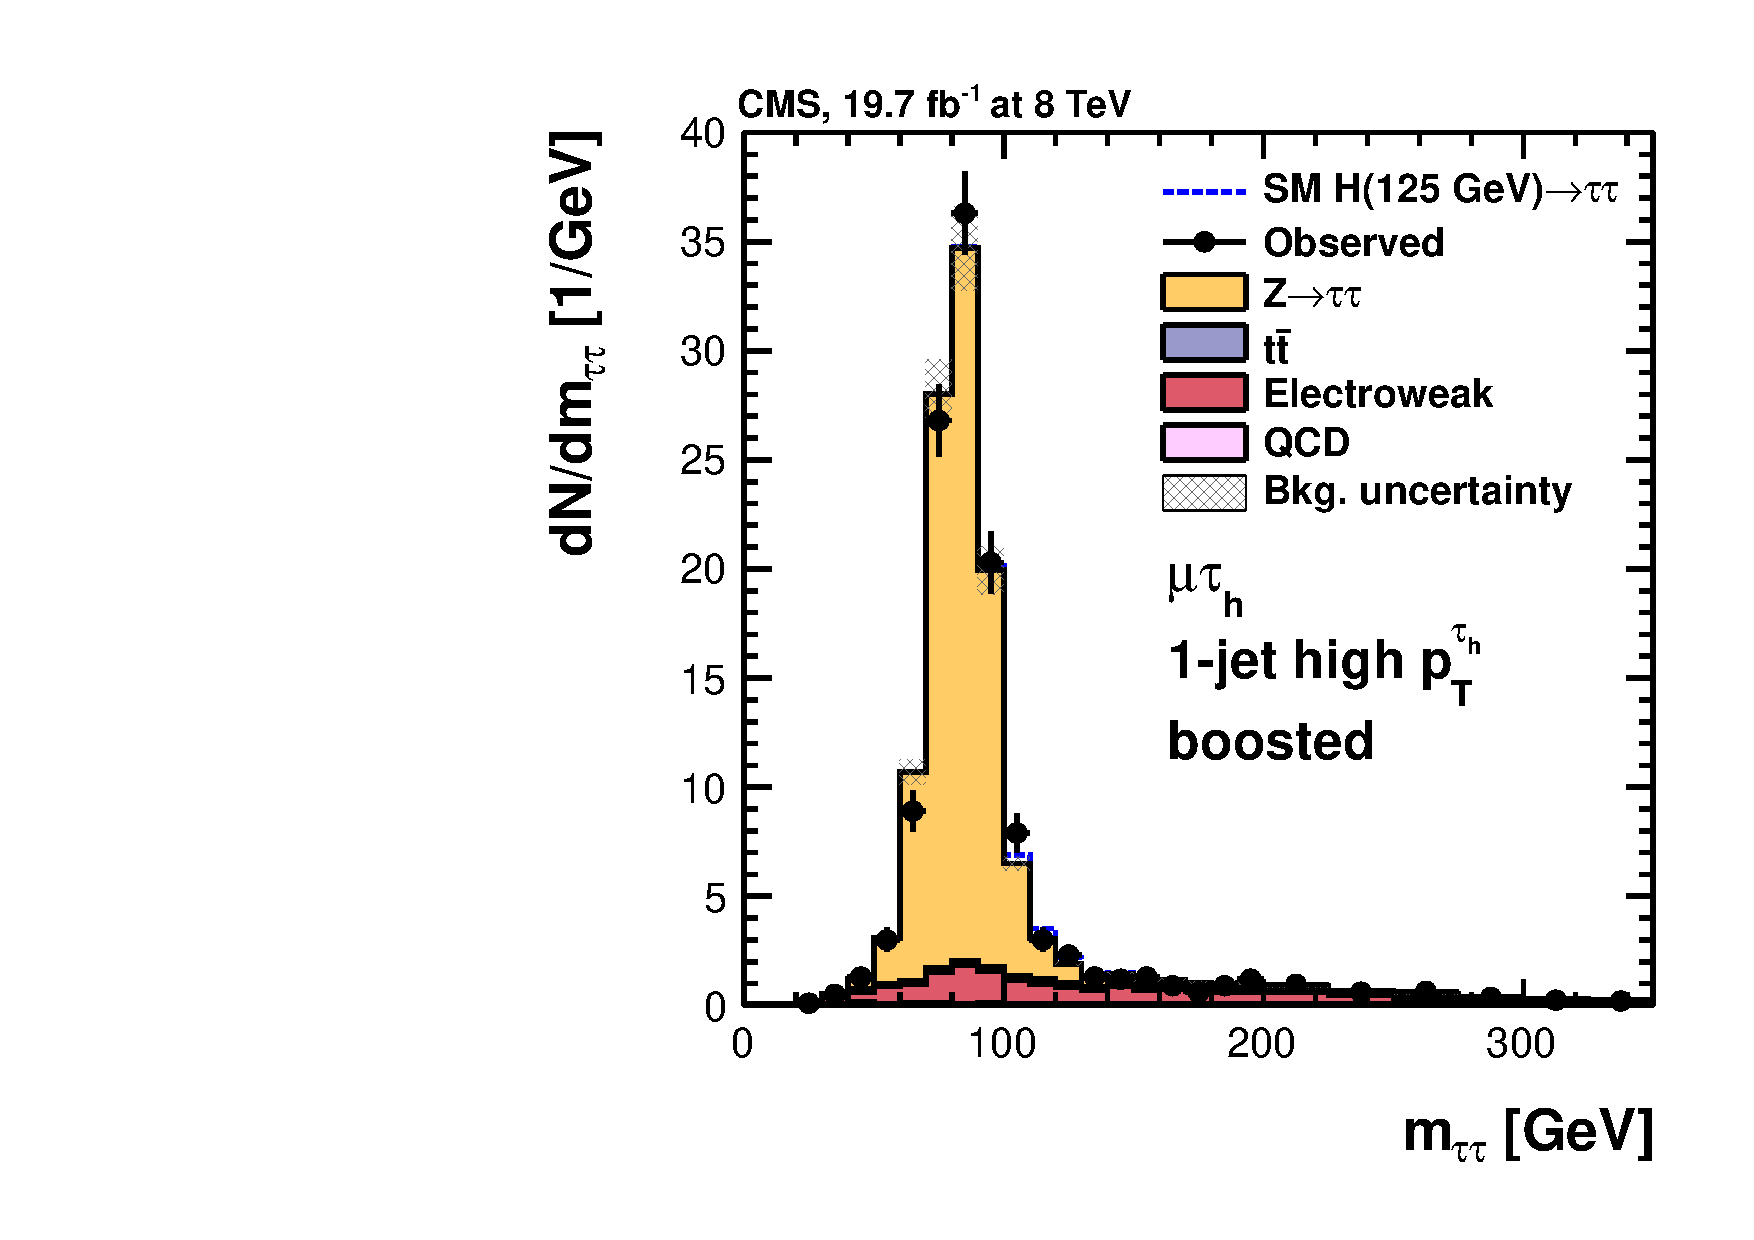
\includegraphics[width=0.5\textwidth]{plots/htt-sm/muTau_1jet_high_mediumhiggs_postfit_8TeV_LIN.pdf}}
\subfloat[]{
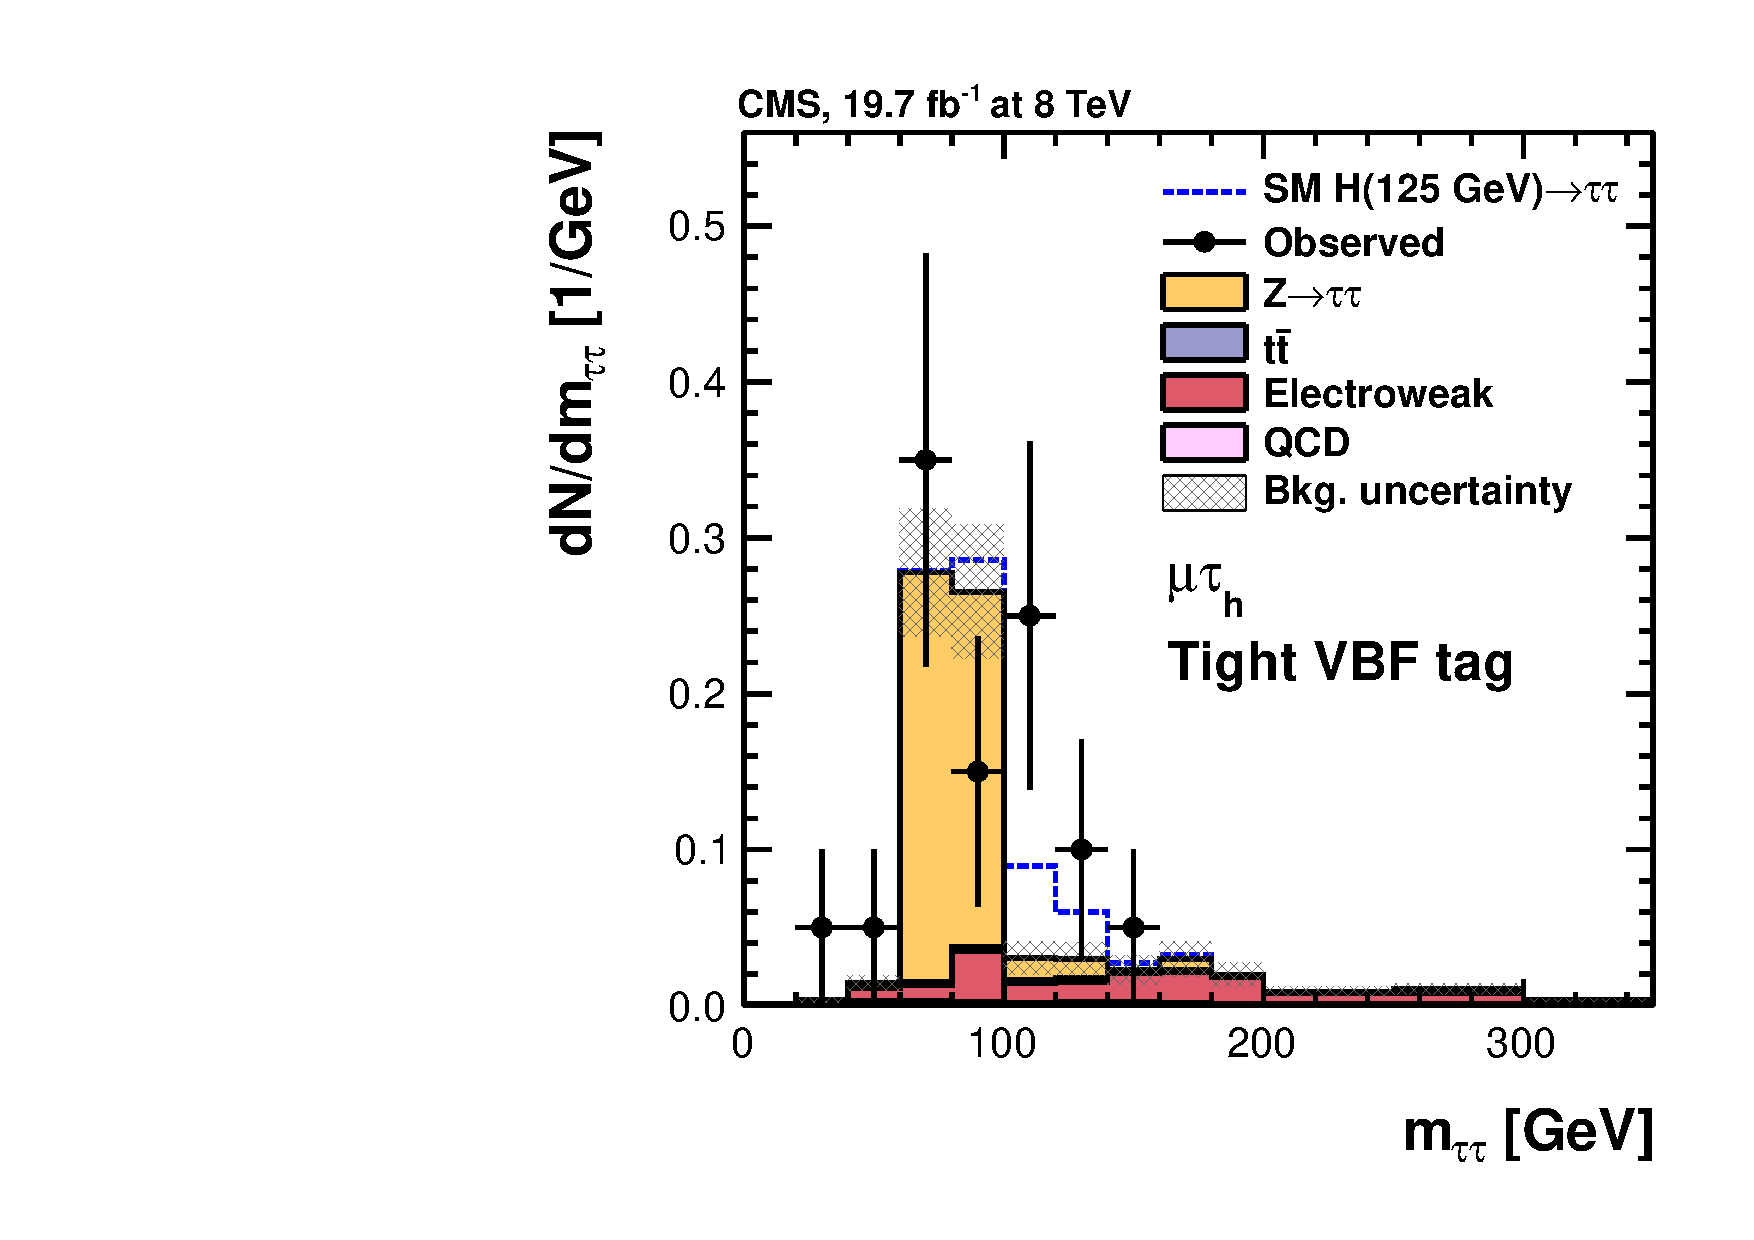
\includegraphics[width=0.5\textwidth]{plots/htt-sm/muTau_vbf_tight_postfit_8TeV_LIN.pdf}}

\subfloat[]{
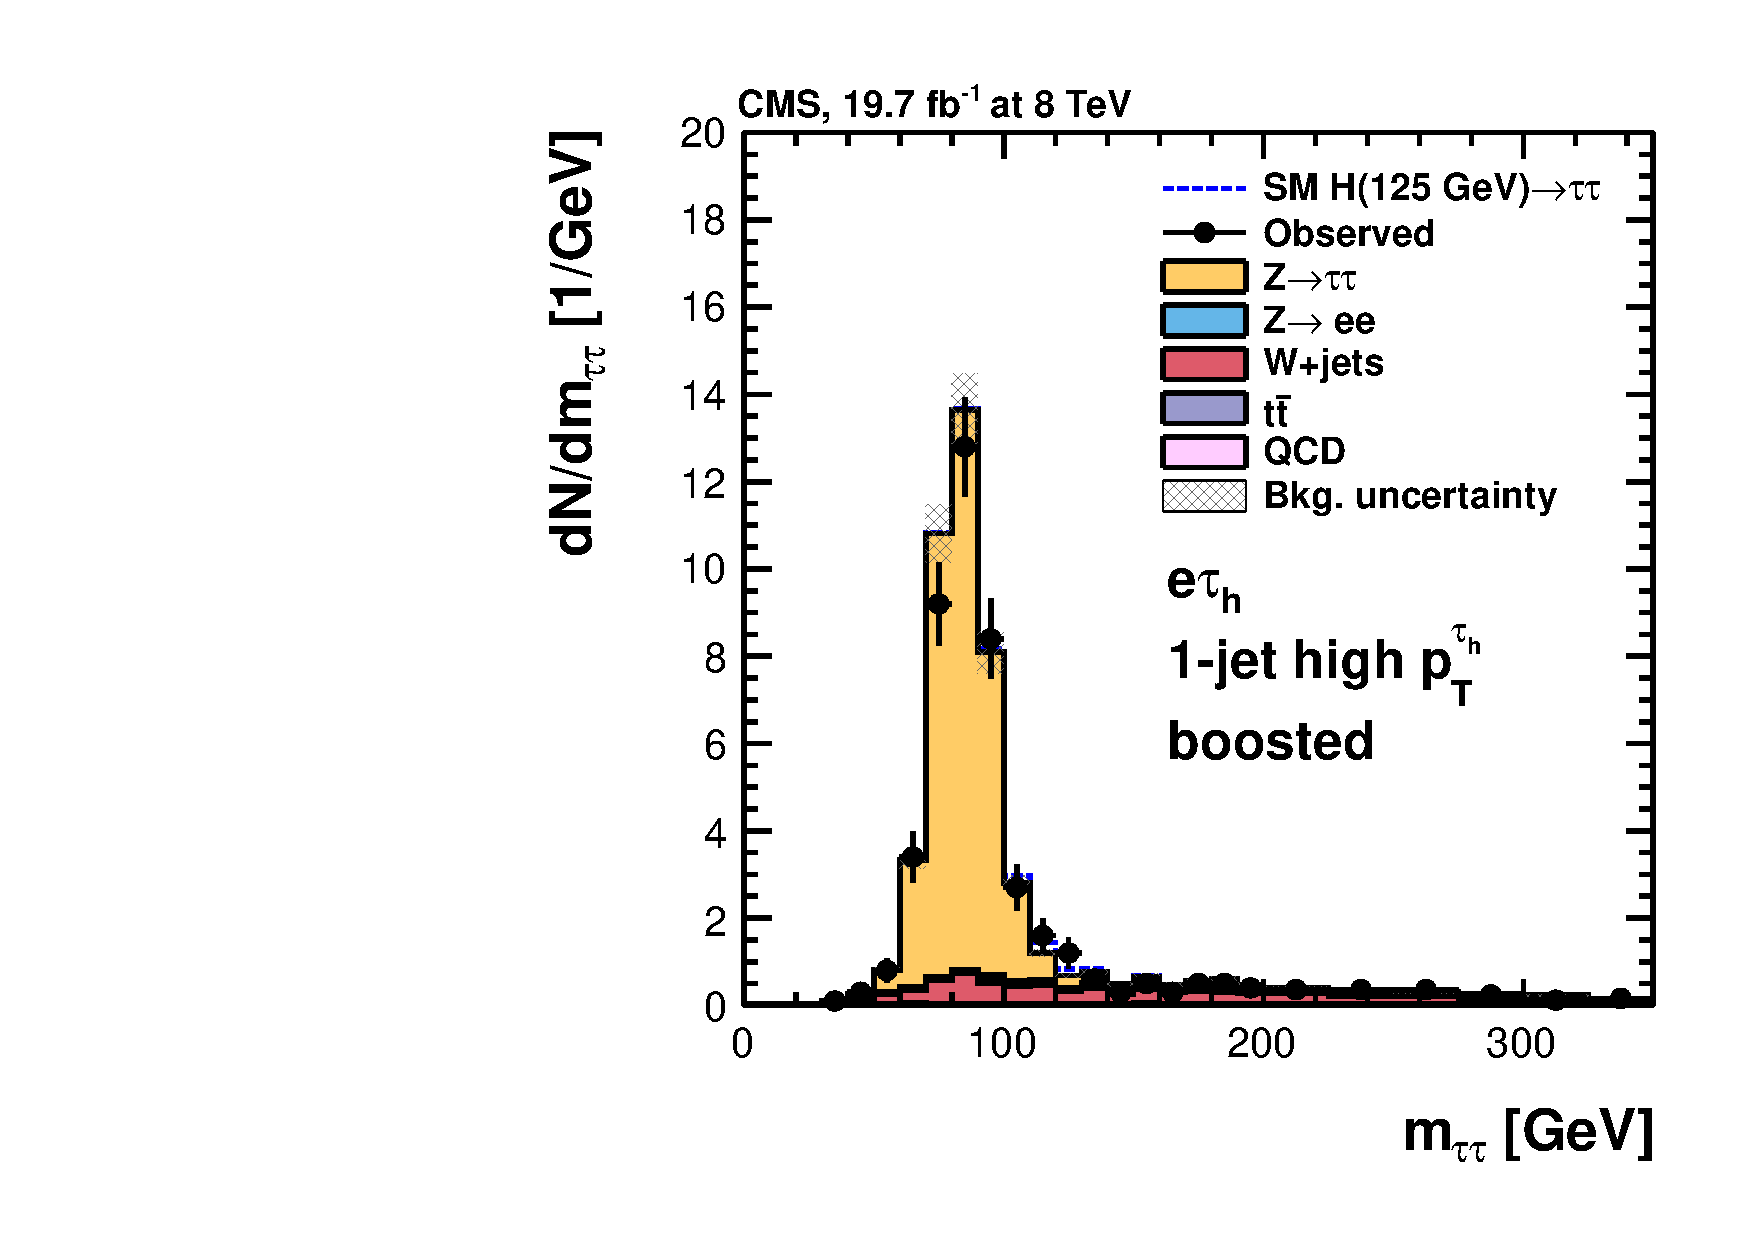
\includegraphics[width=0.5\textwidth]{plots/htt-sm/eleTau_1jet_high_mediumhiggs_postfit_8TeV_LIN.pdf}}
\subfloat[]{
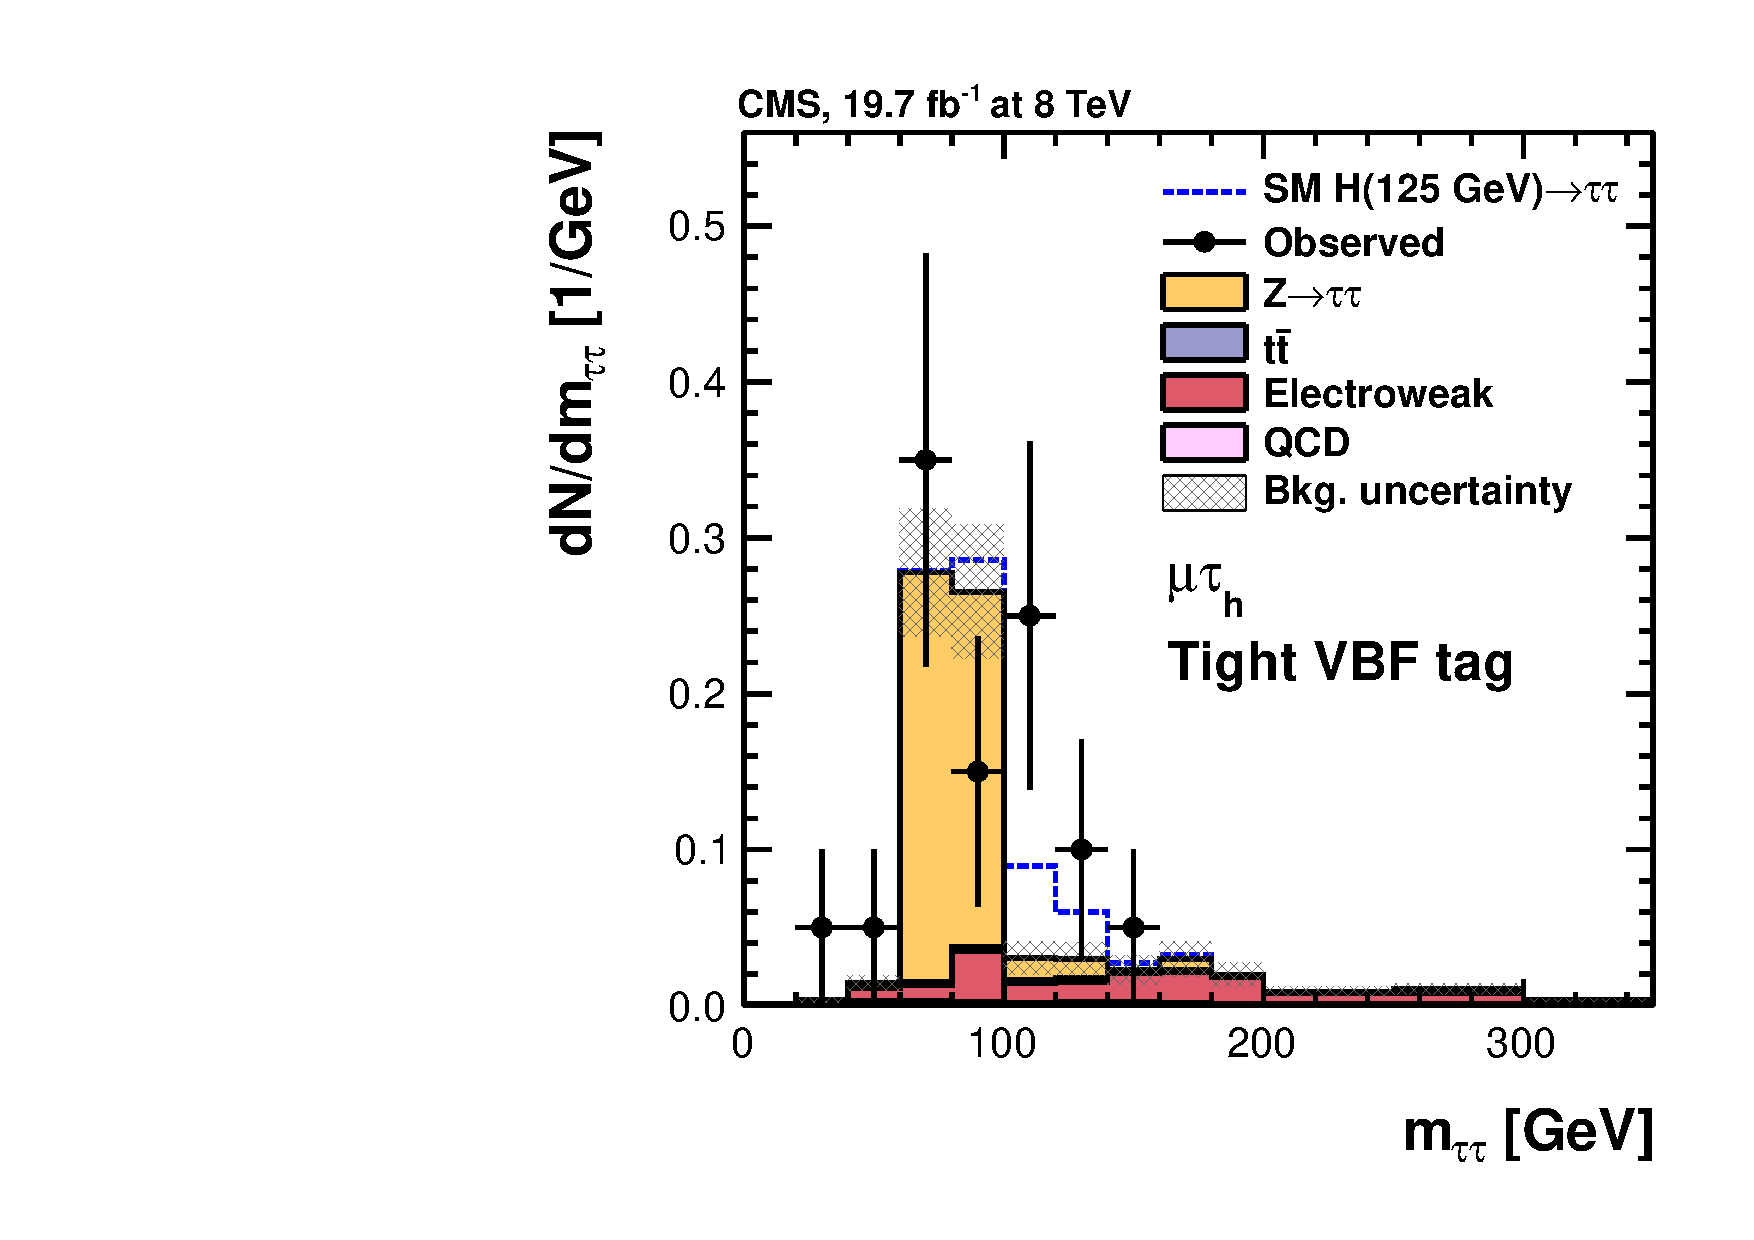
\includegraphics[width=0.5\textwidth]{plots/htt-sm/muTau_vbf_tight_postfit_8TeV_LIN.pdf}}
\caption{Post-fit $m_{\Pgt\Pgt}$ distributions for the 1-jet high
$\pt^{\Pgt_{h}}$ boosted (left) and VBF-tight categories. Plots are shown for
the $\mutau$ channel (top) and $\etau$ channel (bottom) \cite{HIG-13-004}.}
\label{fig:postfitmass}
\end{figure}


\subsection{Limit and Significance}
\label{sec:significance}

The compatibility of the data with either the signal plus background or
background only hypothesis is assessed in terms of the expected and observed
limit and significance from the combination of all channels and categories. The
expected limit can be seen in figure \ref{fig:results-limit}. The left hand plot
shows the expected and observed limit on $\mu$ in the context of the
background-only hypothesis for a range of Higgs mass hypotheses $\mu$. 
It can clearly be seen that the observed limit does not agree with the background 
only hypothesis, indicating an excess in data over the background-only
prediction. The right hand plot compares the same observed limit this time with
an expected prediction that includes a \ac{SM} $125~\GeV$ Higgs. The observed
agrees much more closely with the expected including an \ac{SM} Higgs,
indicating the possible presence of an \ac{SM} Higgs in our data. 

\begin{figure}[h!]
\subfloat[]{
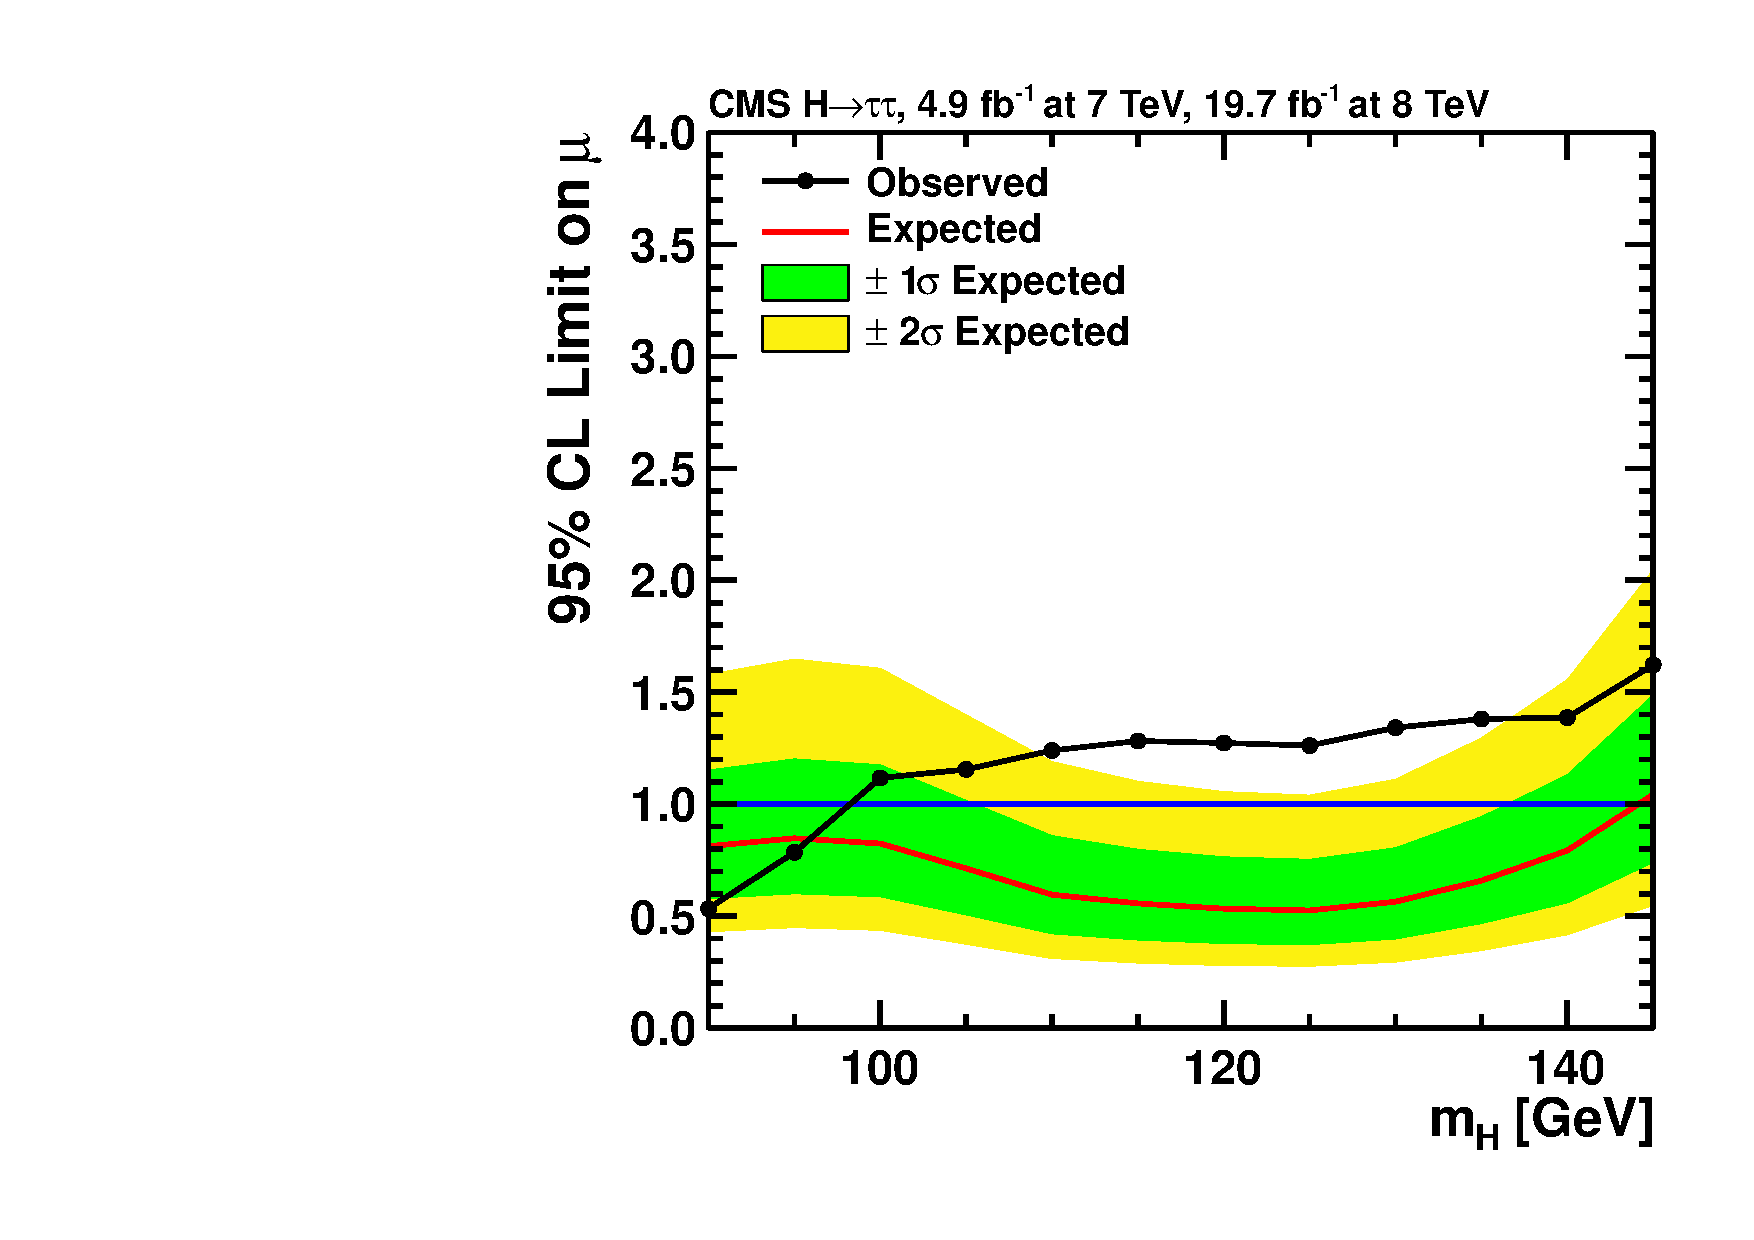
\includegraphics[width=0.5\textwidth]{plots/htt-sm/cmb_limit.pdf}}
\subfloat[]{
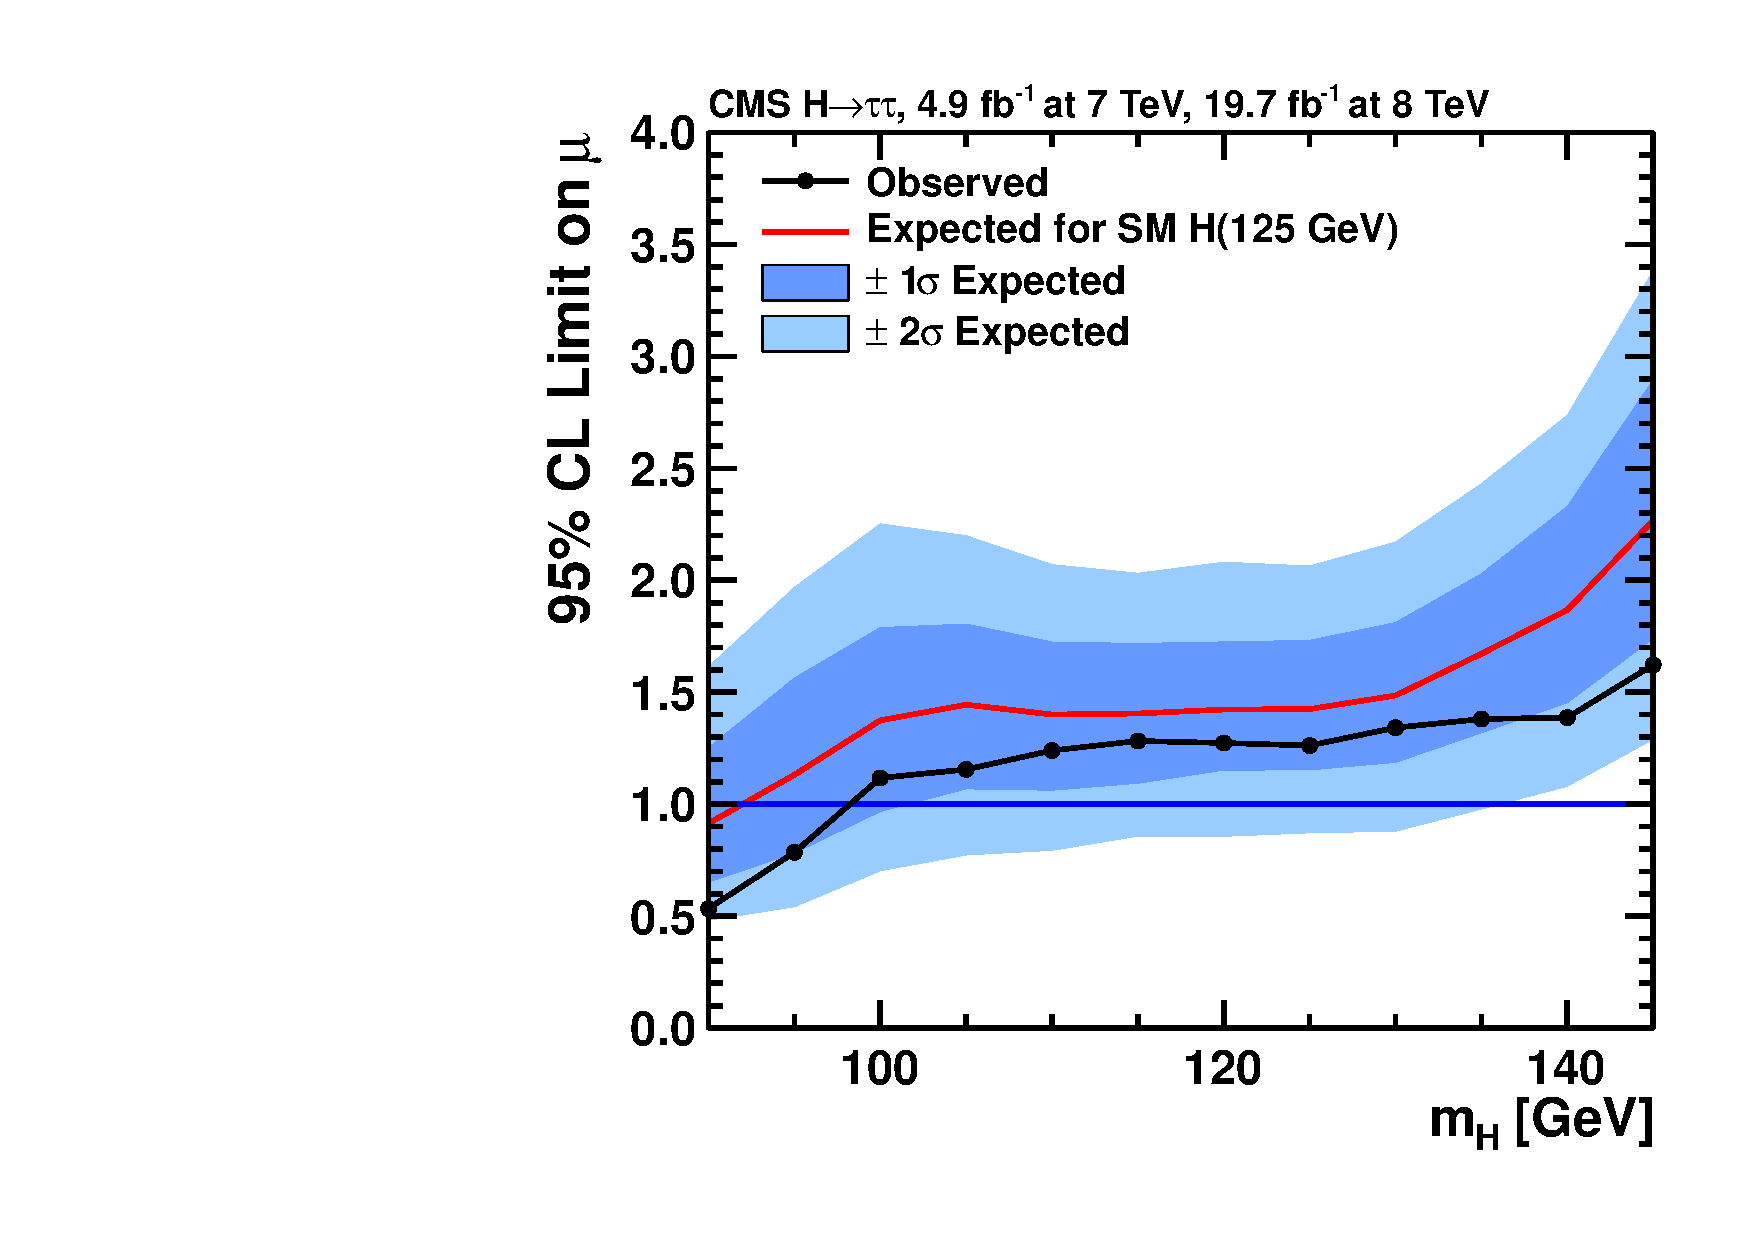
\includegraphics[width=0.5\textwidth]{plots/htt-sm/cmb_limit_signalinjected.pdf}}
\caption{Expected and observed limits obtained using the asymptotic $CL_{s}$
method. The left hand plot compares the observed limit with the expected limit
for the backgroun-only hypothesis, and the right hand plot compares the observed
limit with the expected limit for background only plus \ac{SM} Higgs of
$125~\GeV$ \cite{HIG-13-004}. }
\label{fig:results-limit}
\end{figure}

Figure \ref{fig:results-pvalue} shows the expected and observed significance for
each $m_{\PH}$ hypothesis. The significance is obtained from the p-value by
determining the number of standard deviations of a one-sided normal distribution
which would yield a tail probability of that p-value. The observed (expected)
significance at $125~\GeV$ corresponds to $3.2\sigma$ ($3.7\sigma$). The
significance is larger than $3\sigma$ for values of $m_{\PH}$ between $115~\GeV$
and $130~\GeV$.

\begin{figure}[h!]
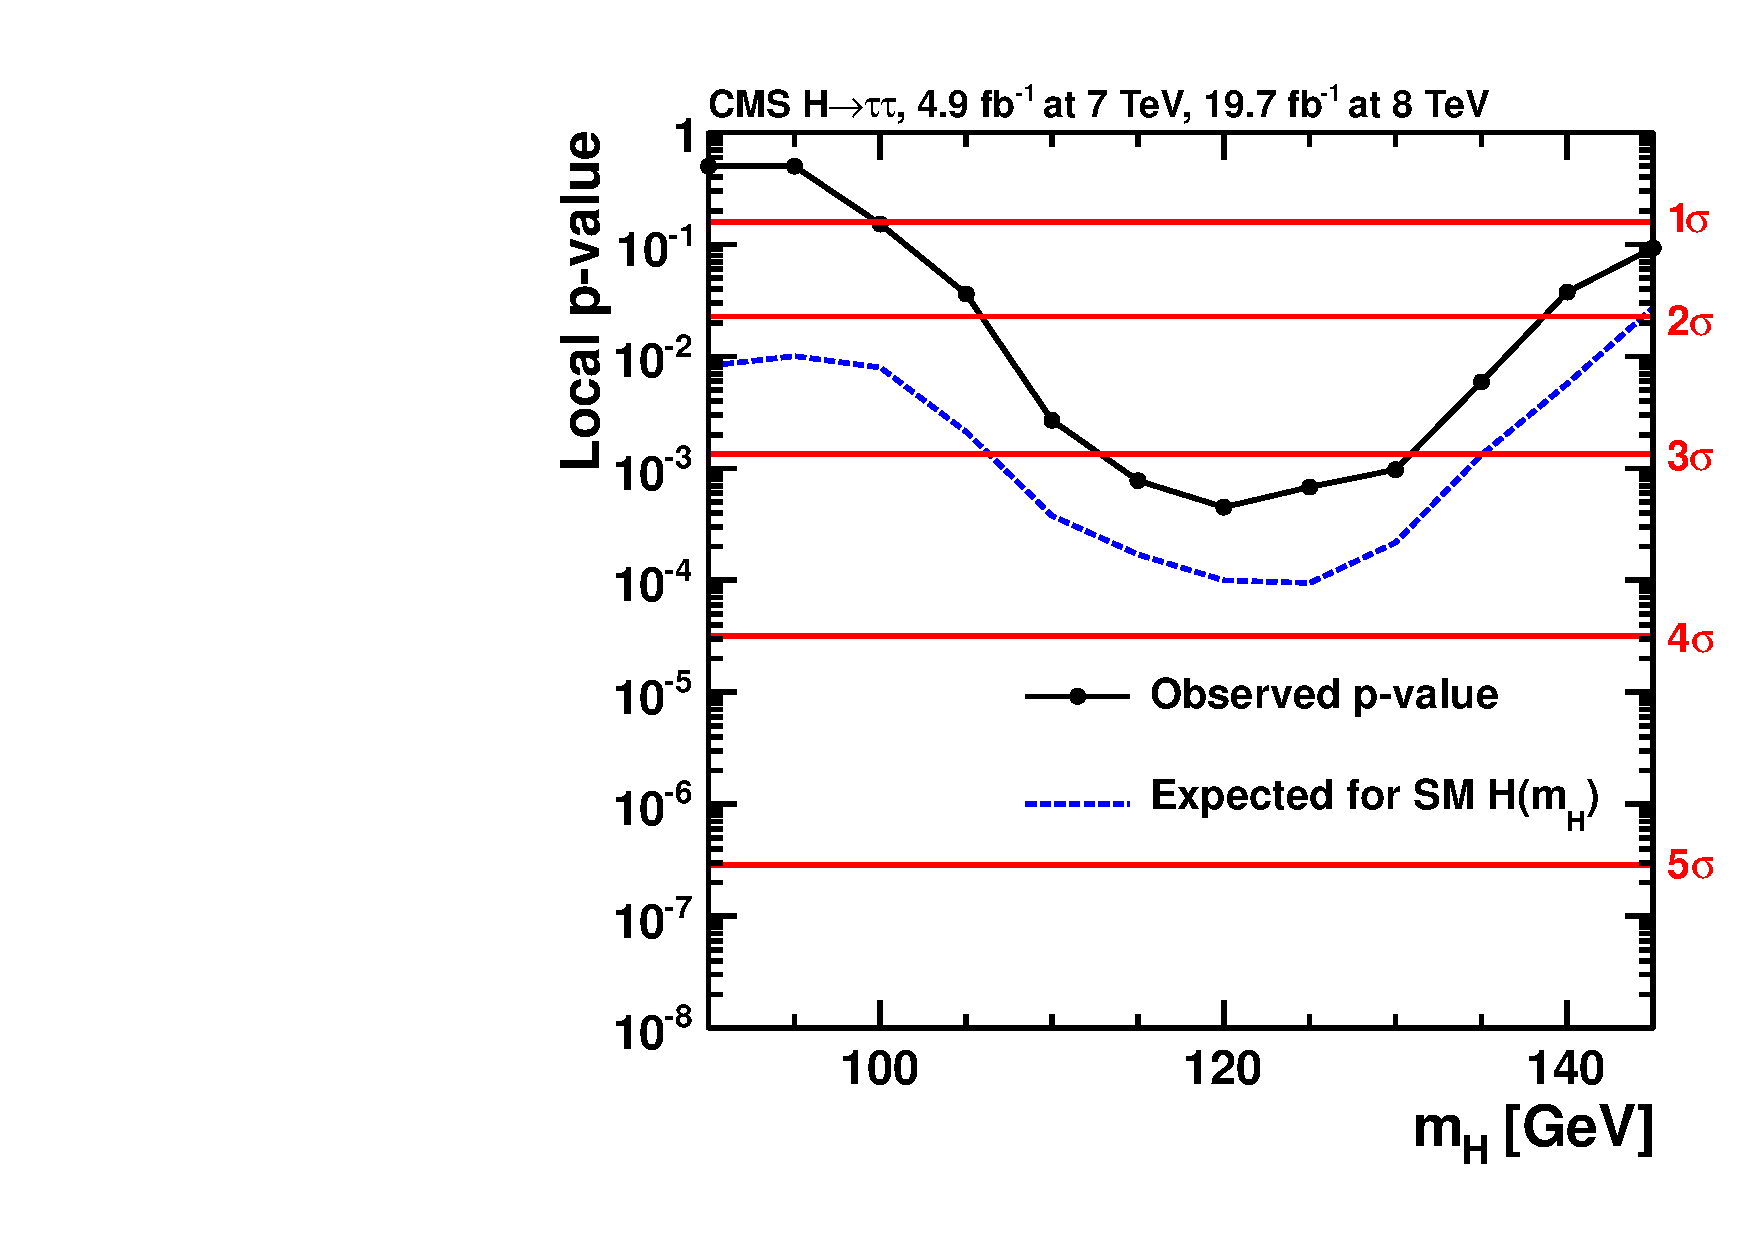
\includegraphics[width=0.5\textwidth]{plots/htt-sm/cmb_p-value.pdf}
\caption{Significance/p-value of the observed data, compared with the expected
significance for an \ac{SM} Higgs boson at each $m_{\PH}$ hypothesis
\cite{HIG-13-004}.}
\label{fig:results-pvalue}
\end{figure}

\subsection{Consistency with $125~\GeV$ Higgs}
\label{sec:consistency}

Having seen that there is an excess in data, the compatibility with a $125~\GeV$
Higgs Boson predicted by the \ac{SM} can be established. From figures
\ref{fig:results-limit} and \ref{fig:results-pvalue}, it can be seen the excess
in data is not only consistent with signal plus background hypothesis for a
$125~\GeV$ Higgs but also for several other masses. Figure
\ref{fig:results-limit} b) already indicates that this is to be expected - it
can clearly be seen that the expected limit for a $125~\GeV$ Higgs is broad
across several mass points, and the observed limit that we see is consistent
with this shape. We can also look at this in the form of a mass scan. Figure
\ref{fig:results-properties} a) shows the value of the observed likelihood at
each mass point compared with the expected likelihood for a $125~\GeV$ \ac{SM}
Higgs boson. The expected distribution of likelihoods is obtained by running
toys with an \ac{SM} Higgs injected, and the 1 and 2 sigma bands come from the
spread in distribution of these toys. A parabolic fit is performed to the
observed values, yielding a best likelihood value at $122~\GeV$. The uncertainty
on this number is obtained from the 1 sigma width of the likelihood curve in
combination with an estimated systematic uncertainty from the energy scales of
the objects, yielding a total uncertainty of $7~\GeV$. Hence the result is
consistent with $125~\GeV$ within the large uncertainty on this measurement,
which is the result of the fact that the di-tau mass resolution is not good
enough to distinguish between values of $m_{\PH}$ any better than this.

The consistency of the excess with a $125~\GeV$ \ac{SM} Higgs also relies on the
Higgs being produced at the predicted rates according to the \ac{SM}
cross-section times branching ratio. Figure \ref{fig:results-properties} b) shows
for a mass of $125~\GeV$ the  best fit values for $\kappa_{f}$ and $\kappa_{V}$,
the couplings to fermions and vector bosons respectively, normalised to the the
\ac{SM} predictions such that the value (1,1) would be perfectly consistent with
the \ac{SM}. The best fit value is shown in the black cross, and the contours
indicate the uncertainty on this value. It can be seen that the couplings are
consistent with the \ac{SM} within the uncertainties.

\begin{figure}[h!]
\subfloat[]{
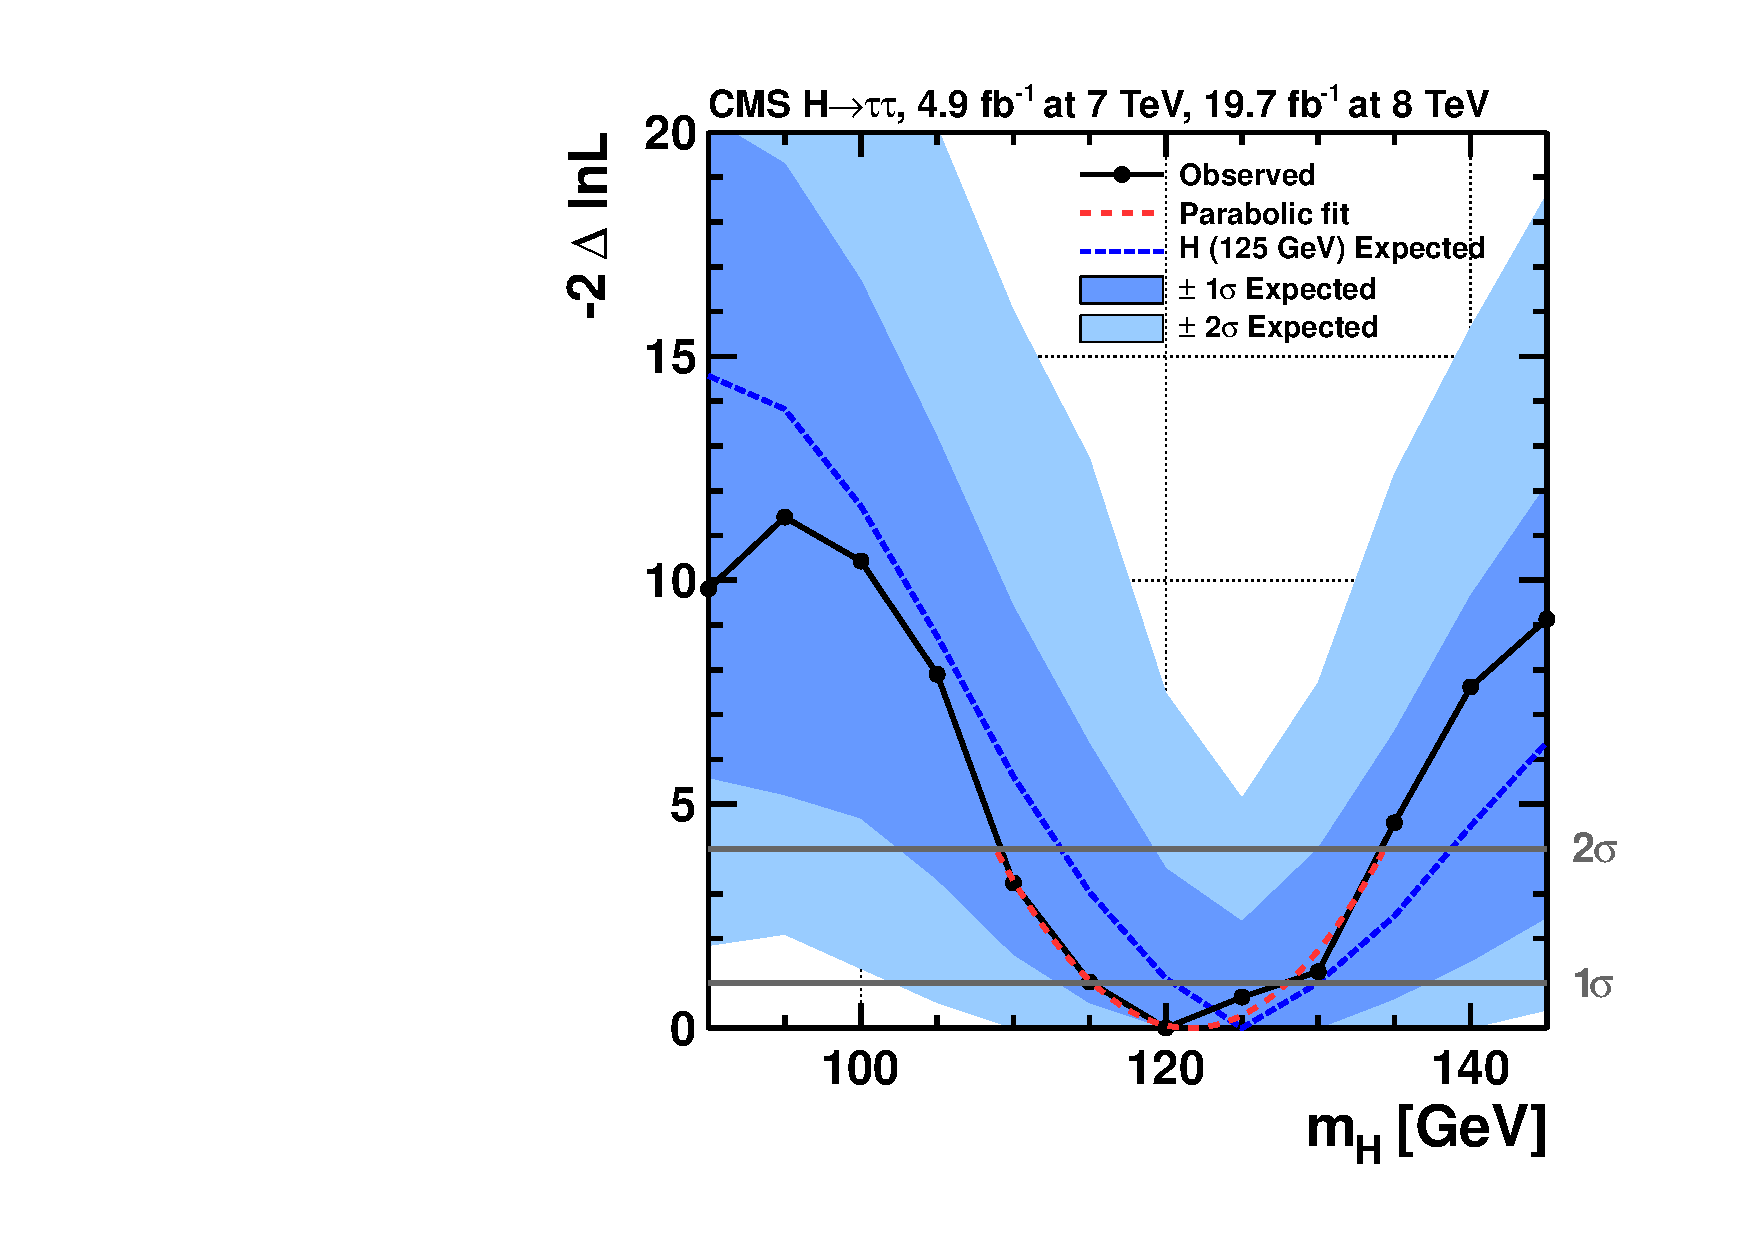
\includegraphics[width=0.5\textwidth]{plots/htt-sm/cmb-mass_scan.pdf}}
\subfloat[]{
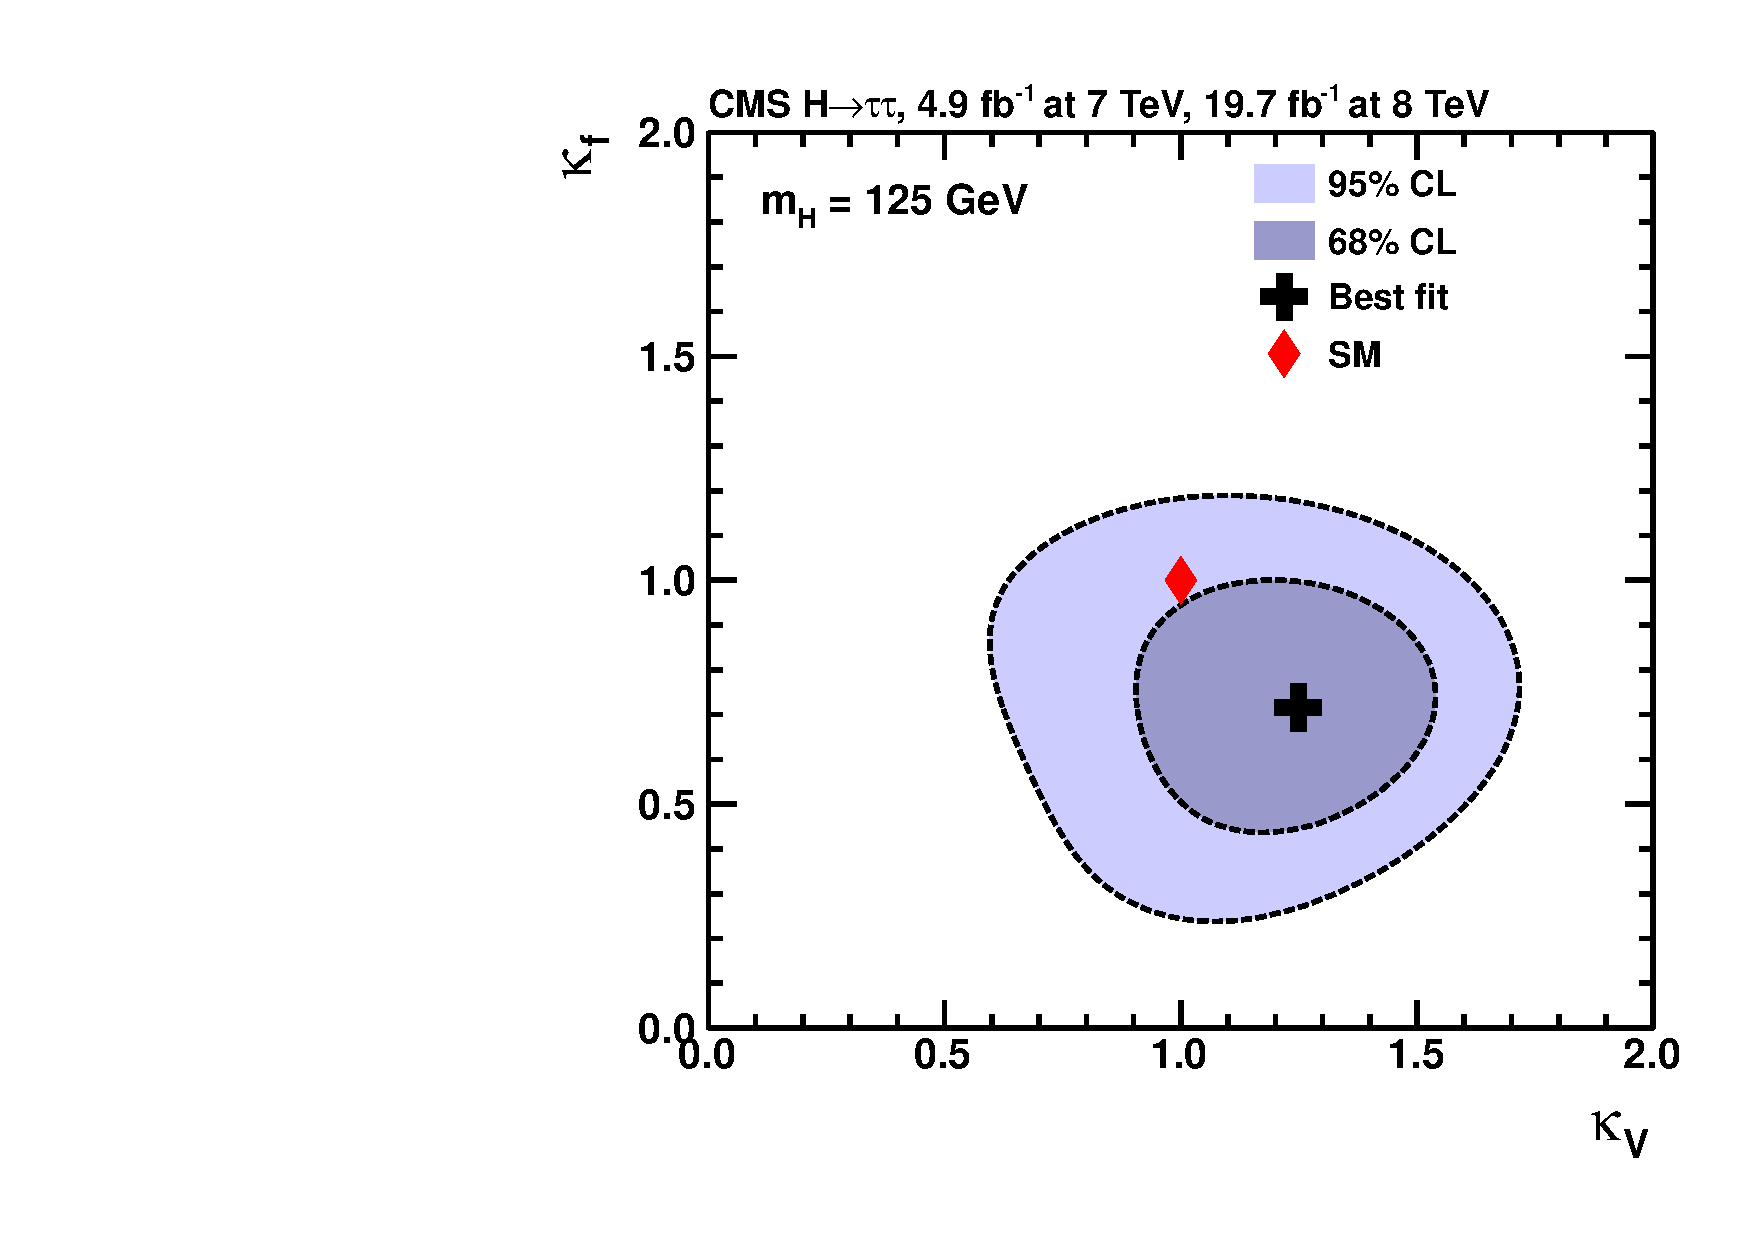
\includegraphics[width=0.5\textwidth]{plots/htt-sm/cmb-scan-hww-CV-CF-125.pdf}}
\caption{Figures indicating the compatibility of the observed excess in data
with a $125~\GeV$ \ac{SM} Higgs Boson. The left hand plot indicates the best fit
value of the mass of the Higgs, and the right hand plot indicates the best fit
value of the couplings to vector bosons and fermions compared with the \ac{SM}
predictions \cite{HIG-13-004}.}
\label{fig:results-properties}
\end{figure}

Hence the data indicates an excess over the background-only prediction which is
consistent with a $125~\GeV$ Higgs boson predicted by the \ac{SM}. The
significance of this excess is larger than $3\sigma$, constituting evidence for
$\HToTauTau$.


